%% abtex2-modelo-trabalho-academico.tex, v-1.9.5 laurocesar
%% Copyright 2012-2015 by abnTeX2 group at http://www.abntex.net.br/ 
%%
%% This work may be distributed and/or modified under the
%% conditions of the LaTeX Project Public License, either version 1.3
%% of this license or (at your option) any later version.
%% The latest version of this license is in
%%   http://www.latex-project.org/lppl.txt
%% and version 1.3 or later is part of all distributions of LaTeX
%% version 2005/12/01 or later.
%%
%% This work has the LPPL maintenance status `maintained'.
%% 
%% The Current Maintainer of this work is the abnTeX2 team, led
%% by Lauro César Araujo. Further information are available on 
%% http://www.abntex.net.br/
%%
%% This work consists of the files abntex2-modelo-trabalho-academico.tex,
%% abntex2-modelo-include-comandos and abntex2-modelo-references.bib
%%

% ------------------------------------------------------------------------
% ------------------------------------------------------------------------
% abnTeX2: Modelo de Trabalho Academico (tese de doutorado, dissertacao de
% mestrado e trabalhos monograficos em geral) em conformidade com 
% ABNT NBR 14724:2011: Informacao e documentacao - Trabalhos academicos -
% Apresentacao
% ------------------------------------------------------------------------
% ------------------------------------------------------------------------

\documentclass[
	% -- opções da classe memoir --
	12pt,				% tamanho da fonte
	%openright,			% capítulos começam em pág ímpar (insere página vazia caso preciso)
	twoside,			% para impressão em verso e anverso. Oposto a oneside
	a4paper,			% tamanho do papel. 
	% -- opções da classe abntex2 --
	%chapter=TITLE,		% títulos de capítulos convertidos em letras maiúsculas
	%section=TITLE,		% títulos de seções convertidos em letras maiúsculas
	%subsection=TITLE,	% títulos de subseções convertidos em letras maiúsculas
	%subsubsection=TITLE,% títulos de subsubseções convertidos em letras maiúsculas
	%pagestart=firstchapter,
	% -- opções do pacote babel --
	english,			% idioma adicional para hifenização
	french,				% idioma adicional para hifenização
	spanish,			% idioma adicional para hifenização
	brazil				% o último idioma é o principal do documento
	]{abntex2}

% ---
% Pacotes básicos 
% ---
\usepackage{subfig}          % figuras lado a lado
\usepackage{lmodern}			% Usa a fonte Latin Modern			
\usepackage[T1]{fontenc}		% Selecao de codigos de fonte.
\usepackage[utf8x]{inputenc}		% Codificacao do documento (conversão automática dos acentos)
\usepackage{lastpage}			% Usado pela Ficha catalográfica
\usepackage{indentfirst}		% Indenta o primeiro parágrafo de cada seção.
\usepackage{color}				% Controle das cores
\usepackage{graphicx}			% Inclusão de gráficos
\usepackage{microtype} 			% para melhorias de justificação
\usepackage{epigraph}
\usepackage{float}
\usepackage{gensymb}

\usepackage{booktabs}
  \usepackage{multirow}
\newcommand{\tabitem}{~~\llap{\textbullet}~~}
\usepackage{amsfonts}
\usepackage[final]{pdfpages}

% Legendas de equacoes
\usepackage{array,tabularx}
\newenvironment{conditions*}
  {\par\vspace{\abovedisplayskip}\noindent
   \tabularx{\columnwidth}{>{$}l<{$} @{\ : } >{\raggedright\arraybackslash}X}}
  {\endtabularx\par\vspace{\belowdisplayskip}}
  \usepackage{amsmath}
% ---
		
% ---
% Pacotes adicionais, usados apenas no âmbito do Modelo Canônico do abnteX2
% ---
\usepackage{lipsum}				% para geração de dummy text
% ---

% ---
% Pacotes de citações
% ---
\usepackage[brazilian,hyperpageref]{backref}	 % Paginas com as citações na bibl
%\usepackage[num]{abntex2cite}	% Citações padrão ABNT
\usepackage[num,nbr14724-2011]{abntex2cite}
\bibliographystyle{abntex2-num}
%\bibliographystyle{ieeetran}

% --- 
% CONFIGURAÇÕES DE PACOTES
% --- 

% ---
% Configurações do pacote backref
% Usado sem a opção hyperpageref de backref
\renewcommand{\backrefpagesname}{Citado na(s) página(s):~}
% Texto padrão antes do número das páginas
\renewcommand{\backref}{}
% Define os textos da citação
\renewcommand*{\backrefalt}[4]{
	\ifcase #1 %
		Sem citações no texto.%
	\or
		Citado na página #2.%
	\else
		Citado #1 vezes nas páginas #2.%
	\fi}%
% ---

% ---
% Informações de dados para CAPA e FOLHA DE ROSTO
% ---
\titulo{Predi\c{c}\~{a}o de Tempo de Vida Restante atrav\'{e}s do aprendizado de m\'{a}quina para condi\c{c}\~{o}es ambientais din\^{a}micas em sistemas integrados}
\autor{Pedro Fausto Rodrigues Leite Junior}
\local{Brasil}
\data{25 de Julho, 2017}
\orientador{Prof. Dr. Frank Sill Torres}
%\coorientador
\instituicao{%
  Universidade Federal de Minas Gerais
  \par
  Programa de Pós-Graduação em Engenharia Elétrica}
\tipotrabalho{Dissertação de Mestrado}
% O preambulo deve conter o tipo do trabalho, o objetivo, 
% o nome da instituição e a área de concentração 
\preambulo{Dissertação apresentada ao programa de Pós-Graduação}

% ---

% ---
% Configurações de aparência do PDF final

% alterando o aspecto da cor azul
\definecolor{blue}{RGB}{41,5,195}

% informações do PDF
\makeatletter
\hypersetup{
     	%pagebackref=true,
		pdftitle={\@title}, 
		pdfauthor={\@author},
    	pdfsubject={\imprimirpreambulo},
	    pdfcreator={LaTeX with abnTeX2},
		pdfkeywords={Confiabilidade}{CMOS}{HCI}{TDDB}{BTI}{Remaing Useful Lifeime}{PLS}, 
		colorlinks=true,       		% false: boxed links; true: colored links
    	linkcolor=black,          	% color of internal links
    	citecolor=black,        		% color of links to bibliography
    	filecolor=black,      		% color of file links
		urlcolor=black,
		%bookmarksdepth=4
}
\makeatother
% --- 

% --- 
% Espaçamentos entre linhas e parágrafos 
% --- 

% O tamanho do parágrafo é dado por:
\setlength{\parindent}{1.3cm}

% Controle do espaçamento entre um parágrafo e outro:
\setlength{\parskip}{0.2cm}  % tente também \onelineskip

% ---
% compila o indice
% ---
\makeindex
% ---
%Colchete
\citebrackets[]

% ----
% Início do documento
% ----
\begin{document}
\raggedbottom
% Seleciona o idioma do documento (conforme pacotes do babel)
%\selectlanguage{english}
\selectlanguage{brazil}

% Retira espaço extra obsoleto entre as frases.
\frenchspacing

% ----------------------------------------------------------
% ELEMENTOS PRÉ-TEXTUAIS
% ----------------------------------------------------------
% \pretextual

%\renewcommand{\imprimircapa}{%
%\begin{capa}%
%    \center
%    \ABNTEXchapterfont\large\imprimirautor
%
%    \vfill
%    \begin{center}
%    \ABNTEXchapterfont\bfseries\LARGE\ An\'{a}lise e Estrat\'{e}gias para Aumento da Robustez em Estruturas com Aut\^{o}matos Celulares de Pontos Qu\^{a}nticos
%    \end{center}
%    \vfill
%    
%    \large\ Brasil
%
%    \large\ 25 de fevereiro de 2016
%    
%    \vspace*{1cm}
%  \end{capa}
%}

% ---
% Capa
% ---
%\imprimircapa

% --
% DESCOMENTAR PARA INSERIR CAPA
%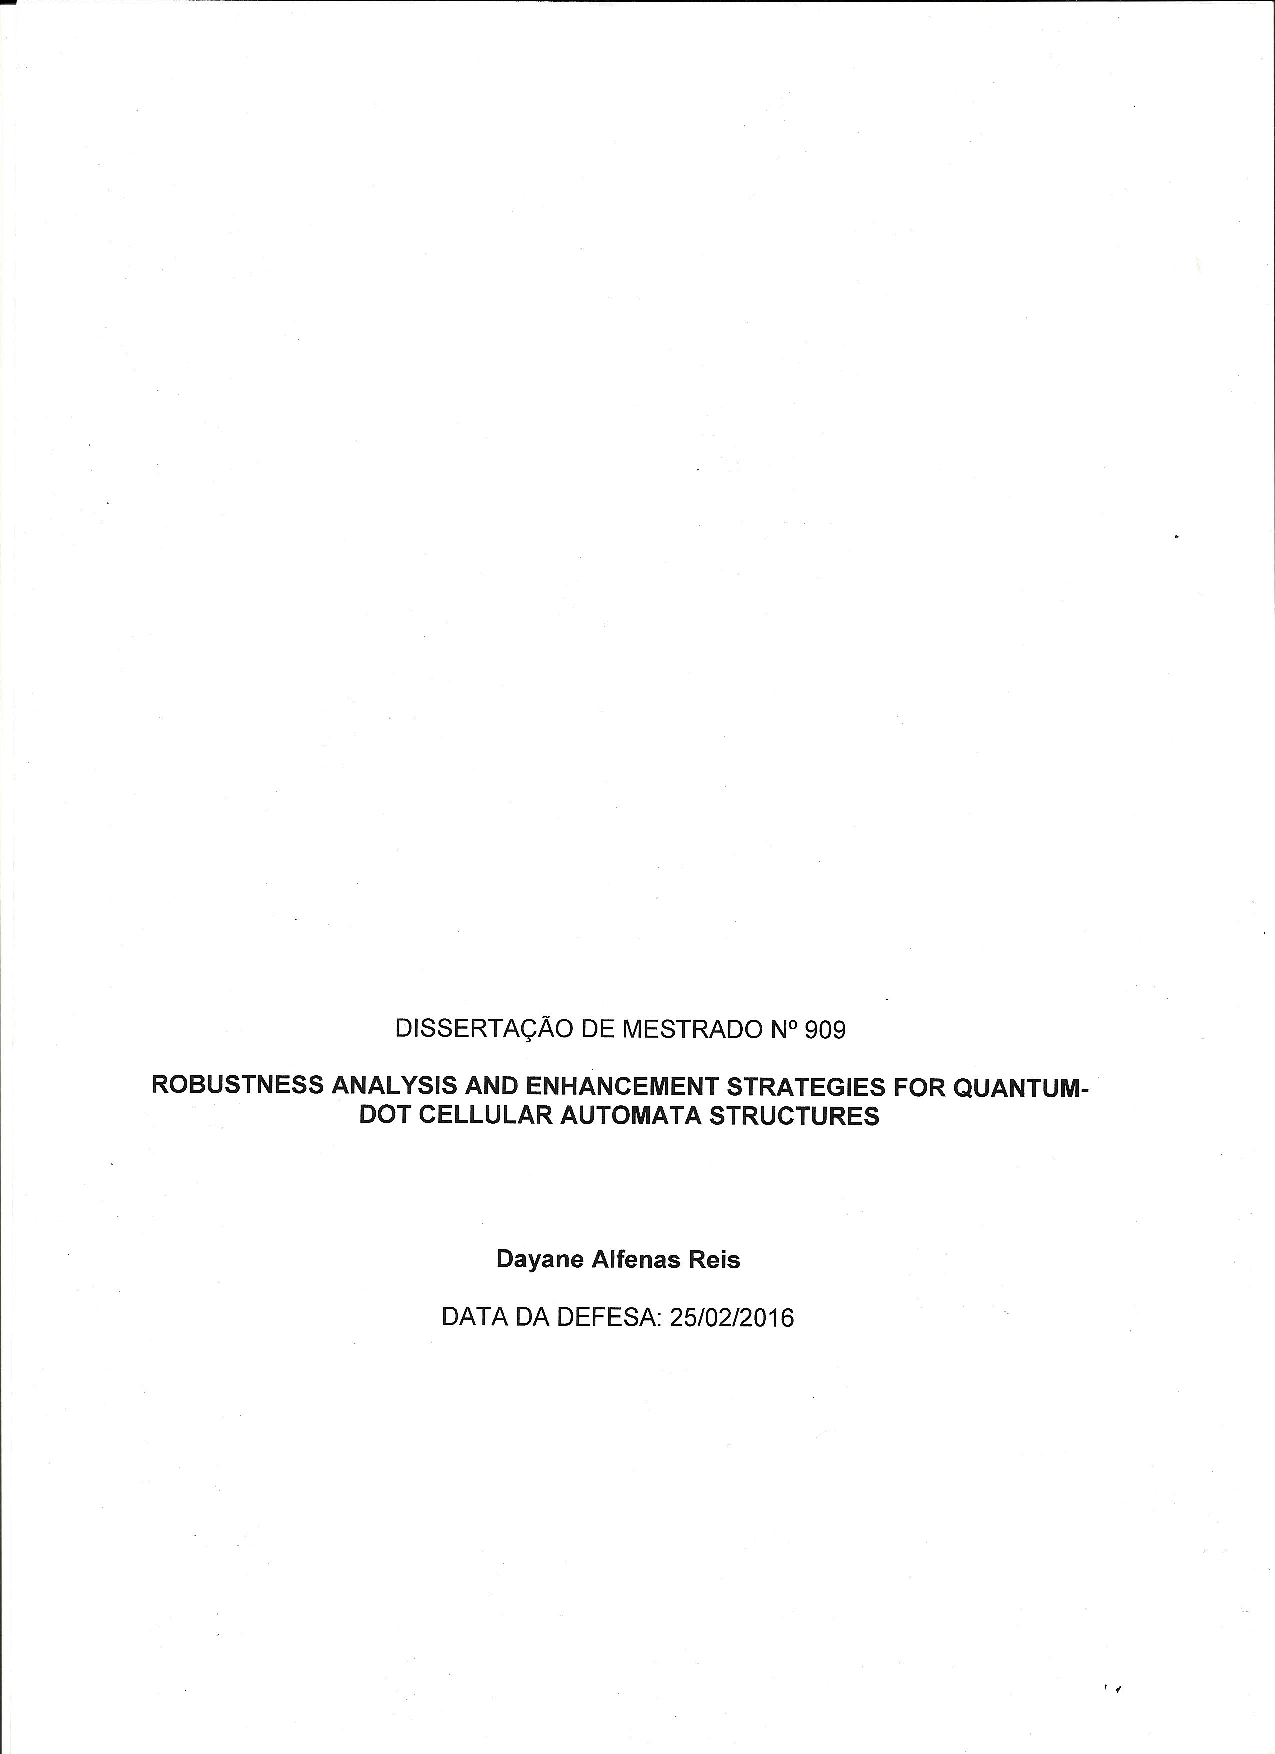
\includepdf[pages={1}]{capa.pdf}
%\renewcommand{\imprimircapa}{%
%\begin{capa}%
%    \center
%    \ABNTEXchapterfont\large\imprimirautor
%
%    \vfill
%    \begin{center}
%    \ABNTEXchapterfont\bfseries\LARGE\imprimirtitulo
%    \end{center}
%    \vfill
%    
%    \large\imprimirlocal
%
%    \large\imprimirdata
%    
%    \vspace*{1cm}
%  \end{capa}
%}

% ---
% Capa
% ---
%\imprimircapa

% ---


% ---
% Folha de rosto
% (o * indica que haverá a ficha bibliográfica)
% ---
%\imprimirfolhaderosto*
% DESCOMENTAR
%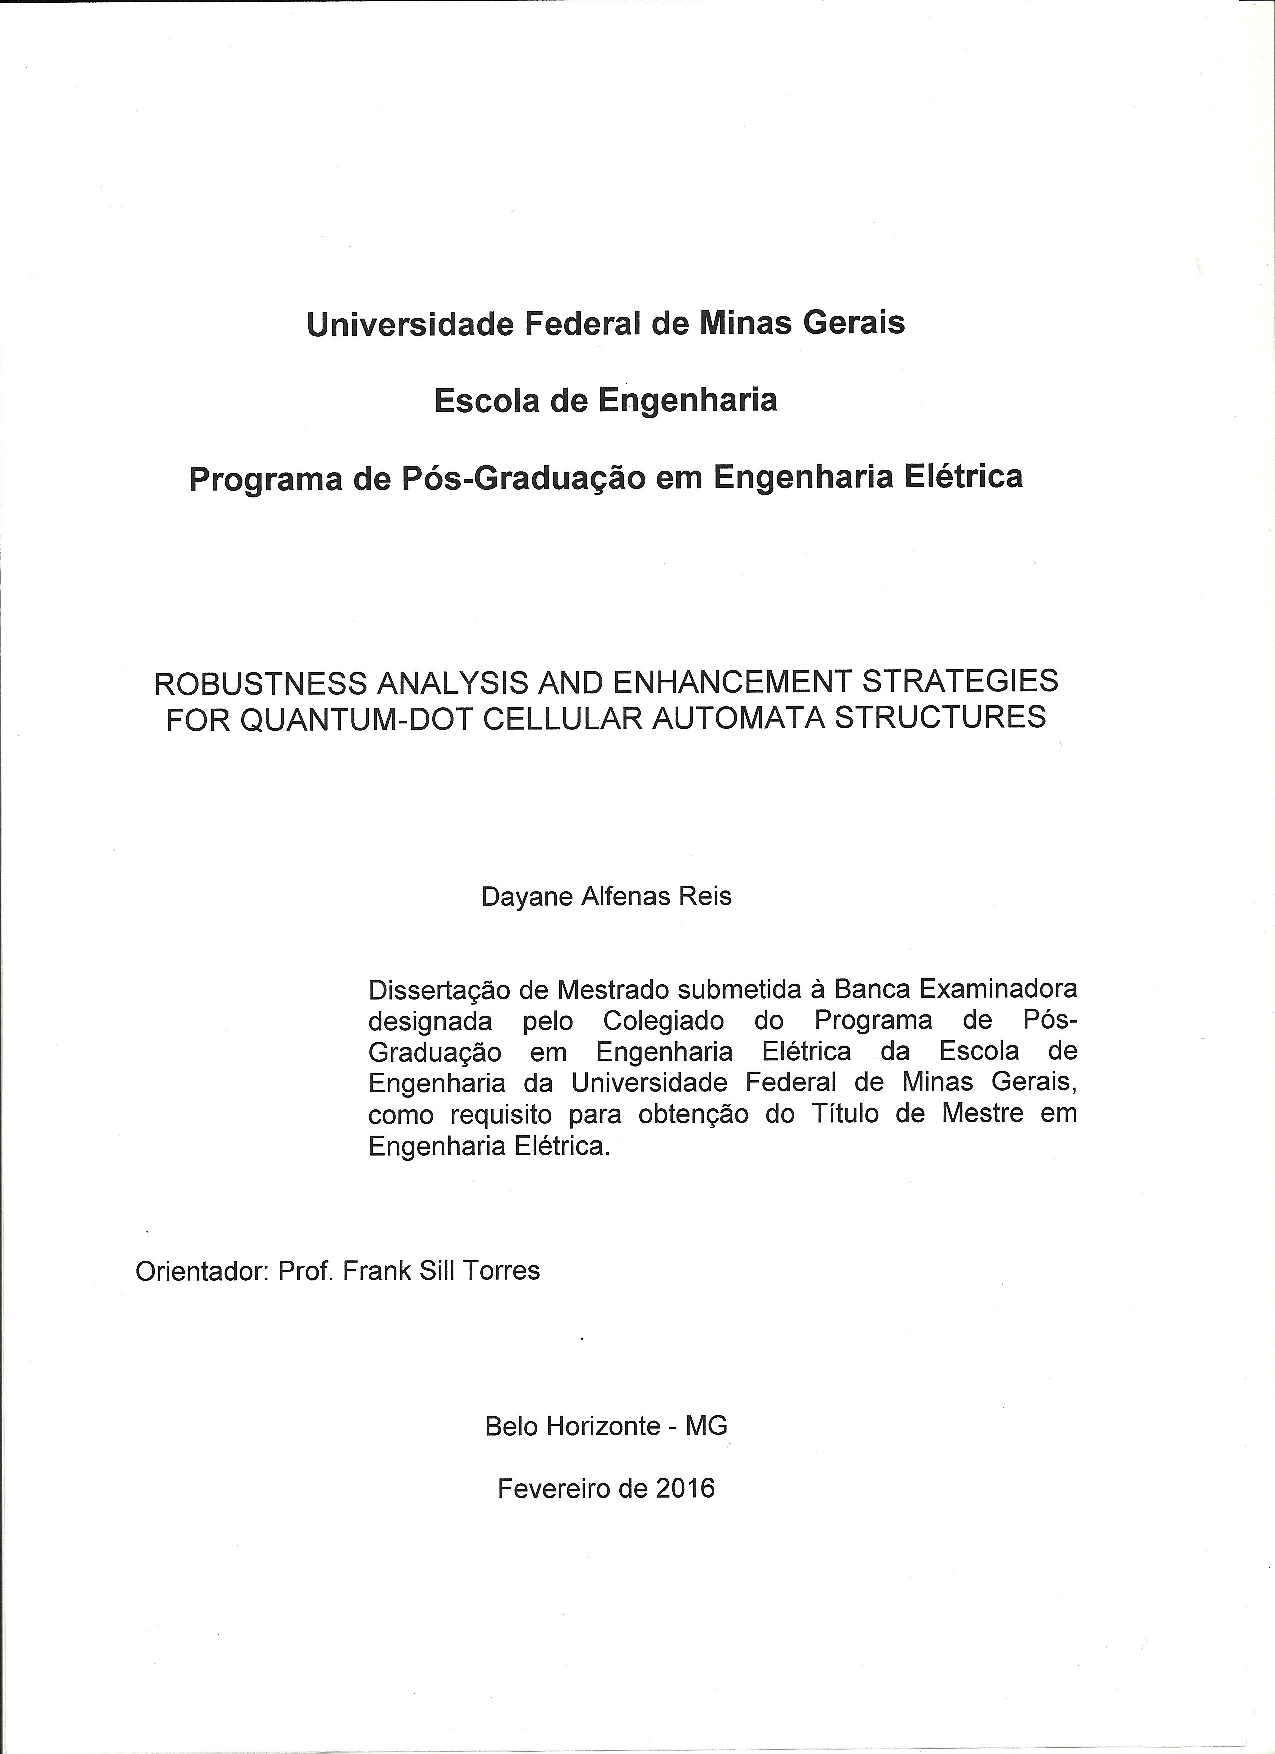
\includepdf[pages={1}]{folha_de_rosto.pdf}
% ---

% ---
% Inserir a ficha bibliografica
% ---

% Isto é um exemplo de Ficha Catalográfica, ou ``Dados internacionais de
% catalogação-na-publicação''. Você pode utilizar este modelo como referência. 
% Porém, provavelmente a biblioteca da sua universidade lhe fornecerá um PDF
% com a ficha catalográfica definitiva após a defesa do trabalho. Quando estiver
% com o documento, salve-o como PDF no diretório do seu projeto e substitua todo
% o conteúdo de implementação deste arquivo pelo comando abaixo:
%
%DESCOMENTAR
%\begin{fichacatalografica}
%     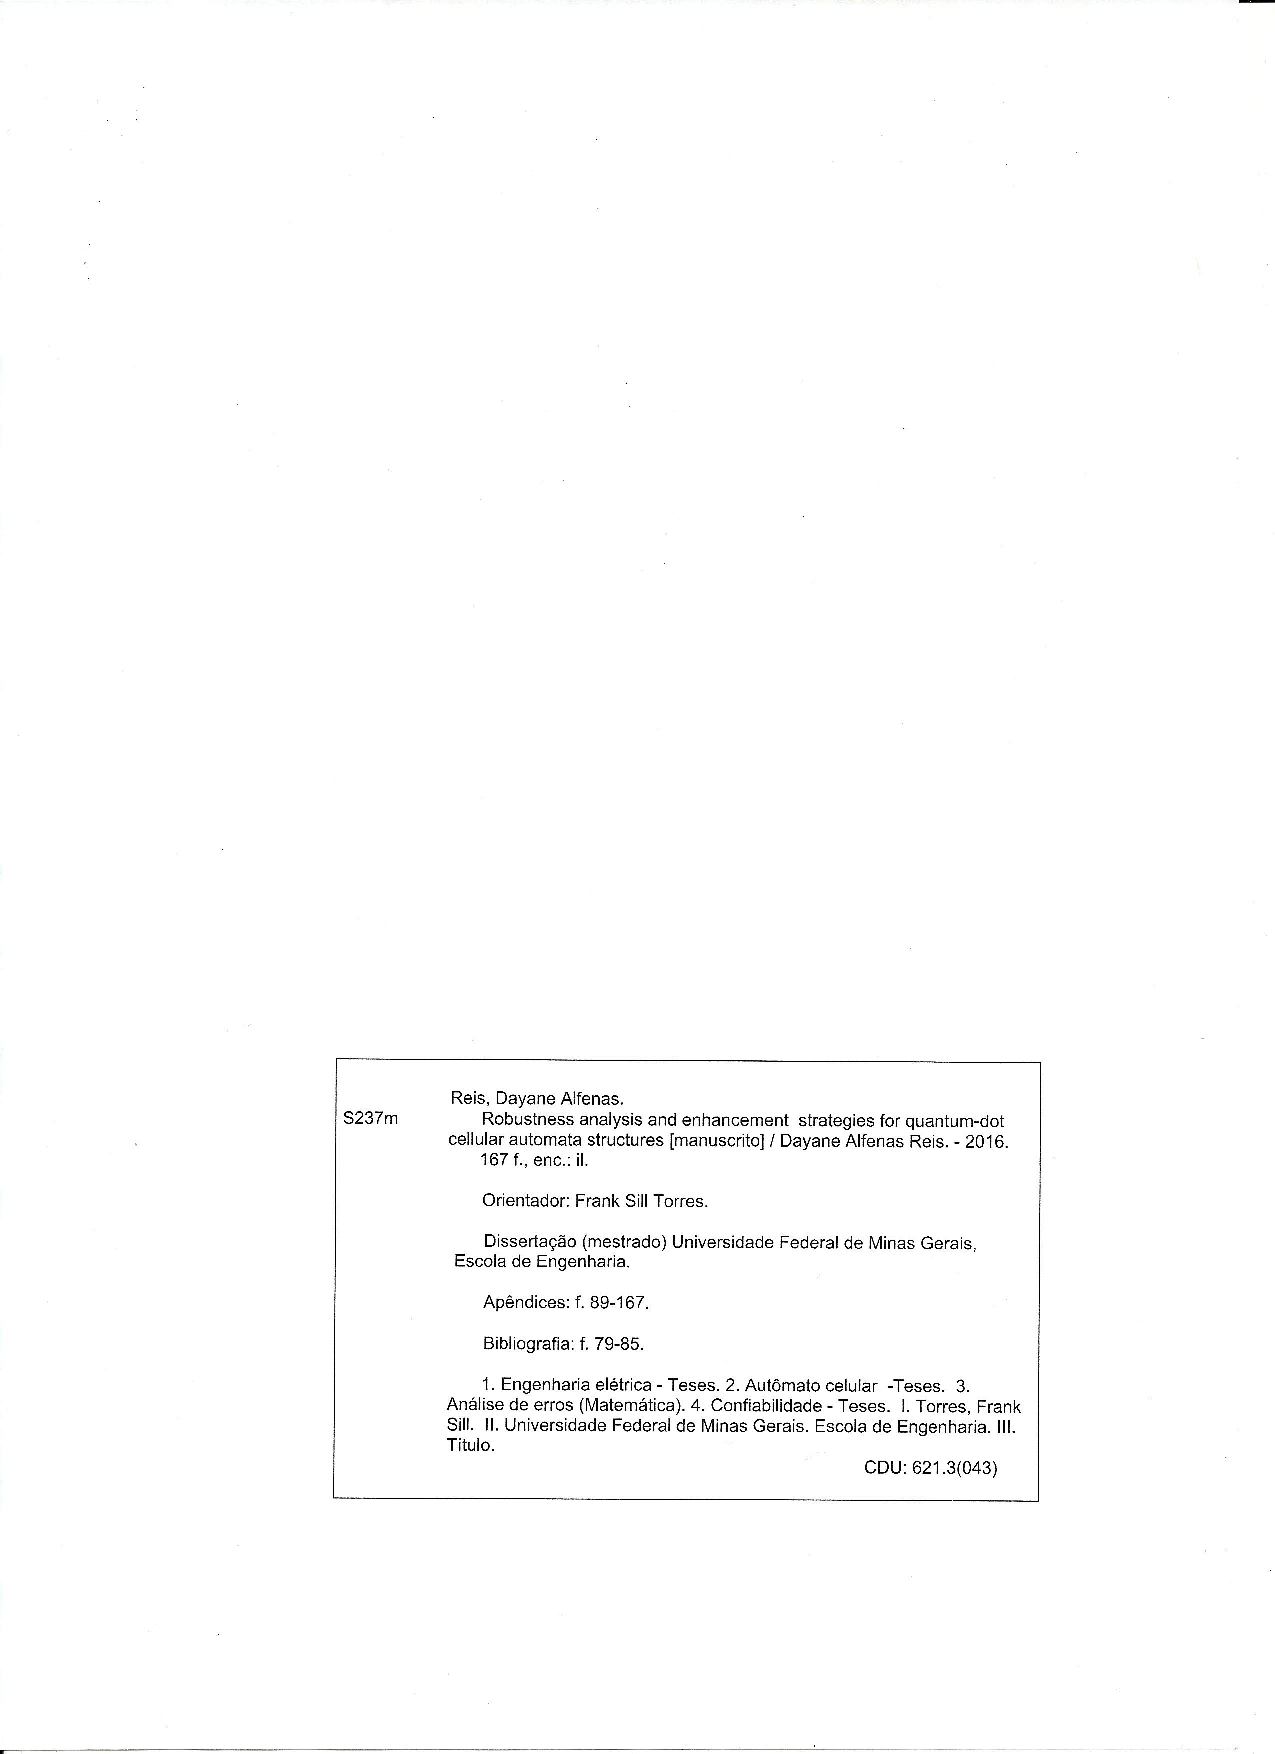
\includepdf{ficha_catalografica.pdf}
%\end{fichacatalografica}

\begin{fichacatalografica}
\sffamily
\vspace*{\fill}					% Posição vertical
\begin{center}					% Minipage Centralizado
\fbox{\begin{minipage}[c][8cm]{13.5cm}		% Largura
\small
\imprimirautor
%Sobrenome, Nome do autor

\hspace{0.5cm} \imprimirtitulo  / \imprimirautor. --
\imprimirlocal, \imprimirdata-

\hspace{0.5cm} \pageref{LastPage} p. : il. (algumas color.) ; 30 cm.\\

\hspace{0.5cm} \imprimirorientadorRotulo~\imprimirorientador\\

\hspace{0.5cm}
\parbox[t]{\textwidth}{\imprimirtipotrabalho~--~\imprimirinstituicao,
\imprimirdata.}\\

\hspace{0.5cm}
	1. Reliability.
	2. Robustness.
	2. Remaning Useful Lifetime.
	I. Frank Sill Torres.
	II. Universidade Federal de Minas Gerais.
	III. Programa de P\'{o}s-Gradua\c{c}\~{o}o em Engenharia El\'{e}trica.
	IV. Predição de Tempo de Vida Restante através do aprendizado de máquina para condições ambientais dinâmicas em sistemas integrados.
	
\end{minipage}}
\end{center}
\end{fichacatalografica}
---

% ---
% ---
% Inserir folha de aprovação
% ---

% Isto é um exemplo de Folha de aprovação, elemento obrigatório da NBR
% 14724/2011 (seção 4.2.1.3). Você pode utilizar este modelo até a aprovação
% do trabalho. Após isso, substitua todo o conteúdo deste arquivo por uma
% imagem da página assinada pela banca com o comando abaixo:
%

%
%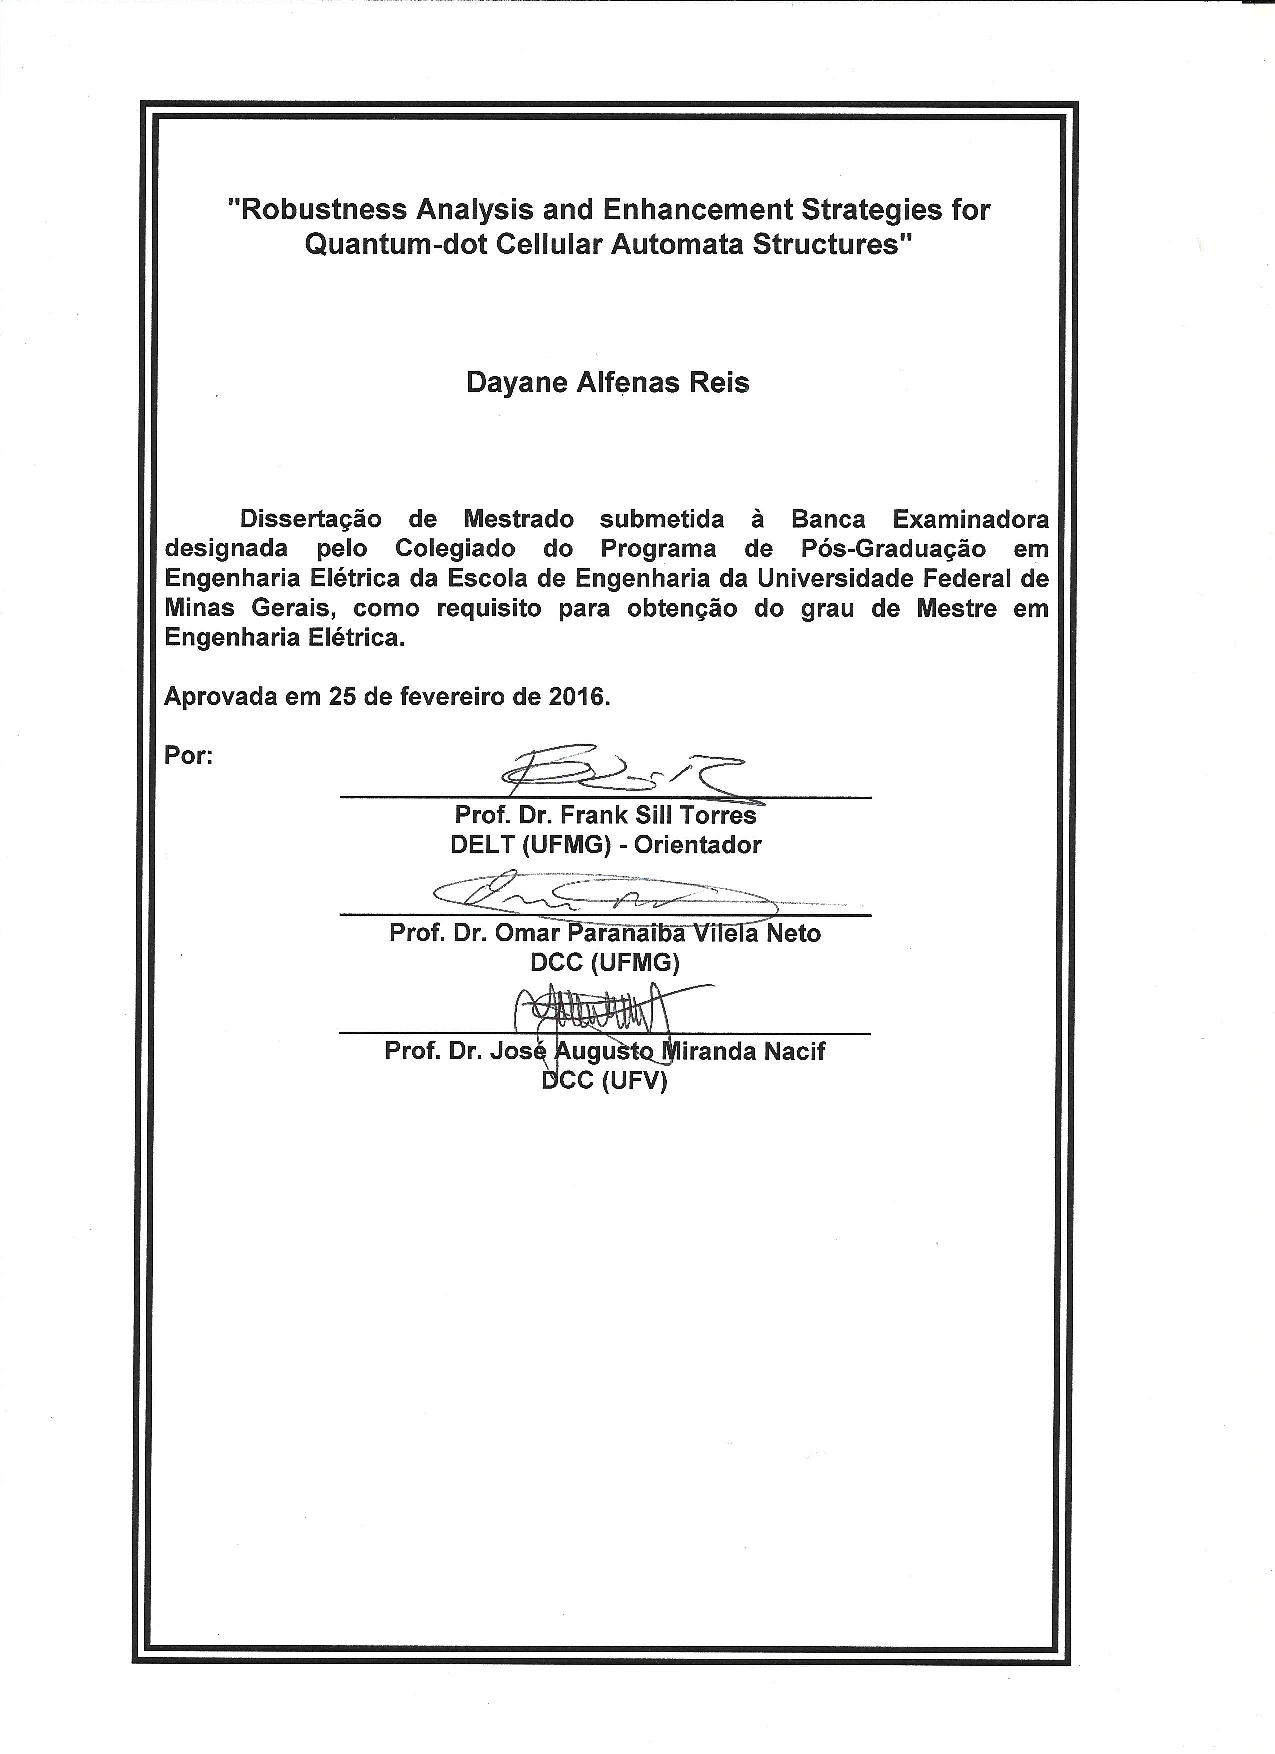
\includegraphics[page=1]{folha_aprovacao.pdf}
%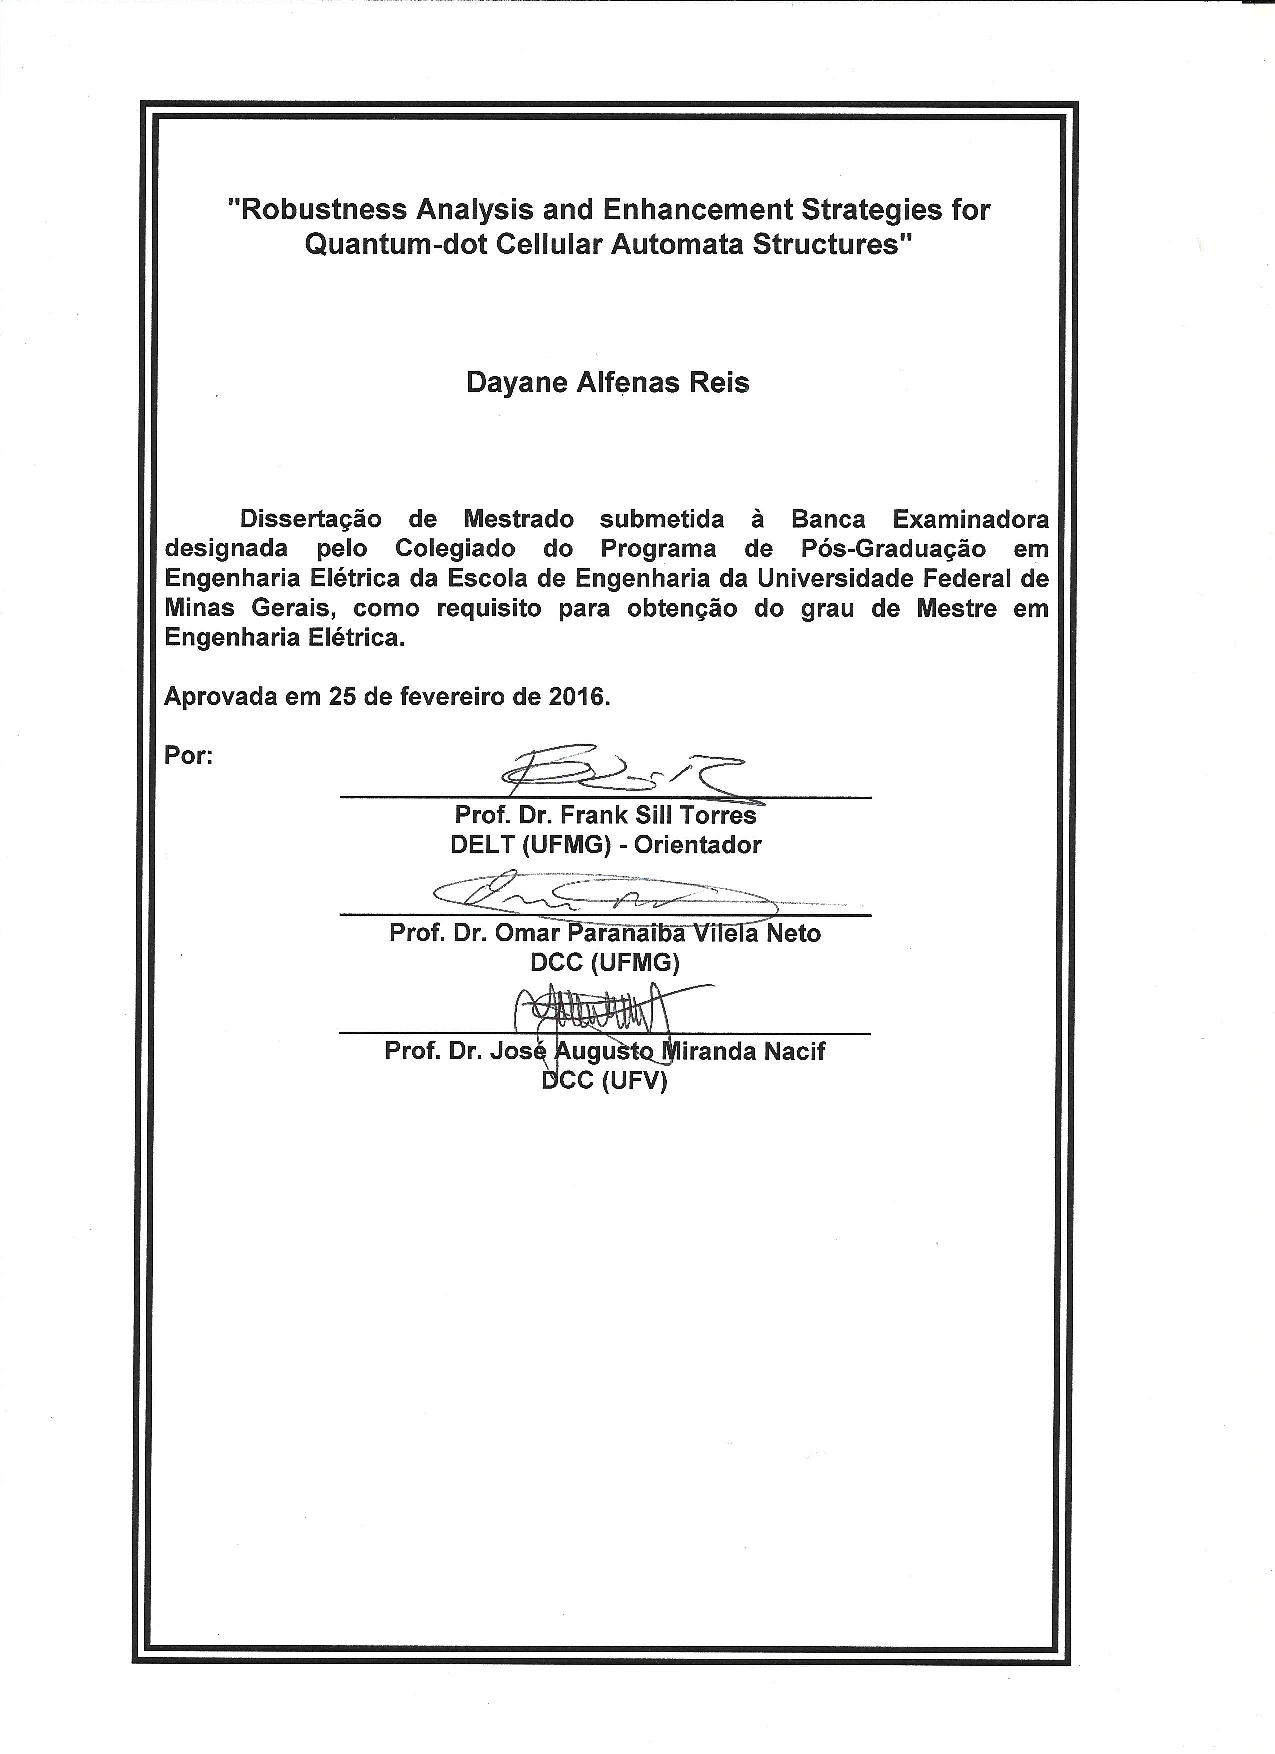
\includepdf[pages={1}]{folha_aprovacao.pdf}
%
% ---
% Capa
% ---
\renewcommand{\imprimircapa}{%
\begin{capa}%
    \center
    \ABNTEXchapterfont\large\imprimirautor

    \vfill
    \begin{center}
    \ABNTEXchapterfont\bfseries\LARGE\imprimirtitulo
    \end{center}
    \vfill
    
    \large\imprimirlocal

    \large\imprimirdata
    
    \vspace*{1cm}
  \end{capa}
}

\imprimircapa

% ---
% Dedicatória
% ---
%DESCOMENTAR
%\begin{dedicatoria}
%   \vspace*{\fill}
%   \centering
%   \noindent
%   \textit{ To Thiago Fernandes Le\~{a}o and Nicolas Reis Cotrim,\\
%   I hope somehow to inspire you, as your smiles inspire me to try my best every day.} \vspace*{\fill}
%\end{dedicatoria}
% ---

% ---
% Agradecimentos
% ---

\begin{agradecimentos}
Gostaria de agradecer ao meu orientador, Professor Dr. Frank Sill Torres pelo auxílio e ensinamentos. É sempre gratificante poder aprender quando se há alguém disposto a transmitir seu conhecimento. Este trabalho não seria possível sem sua incansável capacidade de ensinar, ajuda e busca pela excelência. E sua compreensão e paciência também.

A todos os membros do $OptMA^{lab}$, agradeço de coração pelas trocas de experiência, incentivos e momentos de alegria que me ajudaram a relaxar, respirar fundo e continuar o trabalho. Mencionar individualmente cada um só diminuiria o valor intrínseco do $OptMA^{lab}$: uma equipe.

Aos demais amigos, muitos, que de uma forma ou de outra me incentivaram durante essa jornada.

À minha família pelo apoio incondicional na labuta diária, me apoiando na minha decisão de voltar à pesquisa científica, sejam quais forem as dificuldades encontradas em um trabalho tão essencial à sociedade mas que ainda há de ganhar o devido reconhecimento.

À Sabrina pelo carinho, companheirismo e por sempre me manter focado no que importa.
\end{agradecimentos}

% ---

% ---
% RESUMOS
% ---
\setlength{\absparsep}{18pt} % ajusta o espaçamento dos parágrafos do resumo
% resumo em português
\begin{resumo}
\begin{otherlanguage*}{brazil}
O estudo da confiabilidade de circuitos integrados tem se tornado de súbita importância para o entendimento, detecção e correção de falhas dos mesmos. A compreensão de como ou sob quais condições este envelhecimento se torna prejudicial a um sistema permitirá tomar decisões que sanem ou evitem estas condições.

Este trabalho estabelece um fluxo para análise e simulação de sistemas integrados que permite entender o envelhecimento dos  mesmos, em diferentes condições. Além disso, permite extrair e analisar dados que são relevantes para prever a falha dos mesmos e sirvam de entrada para sistemas de verificação, avaliação e atuação contra falhas utilizando-se de técnicas de aprendizado de máquina.

A metodologia desenvolvida permite a integração de técnicas de coleta de dados \textit{offline} e \textit{online} para atualização dos métodos de estimativa, além de permitir que novos sejam adicionados. O trabalho utiliza três métodos diferentes para prever o Tempo Médio para Falha (\textit{i.e.} Mean Time To Failure, MTTF) e o Tempo de Vida Restante para alguns circuitos de teste ISCAS-85 e uma cadeia de inversores.
O MTTF é estimado para cada um deles utilizando um Modelo Linear Generalizado (especificamente uma Regressão de Mínimos Quadrados Parciais), a Distância Euclideana e a Correlação de Pearson como métodos de predição.

Os resultados obtidos indicam que a representação das condições de operação dos sistemas através de perfis dinâmicos é mais realística do que a representação através de um perfil de operação que não varia no tempo, além de mais precisa. Adicionalmente, a predição do MTTF foi de aproximadamente 90\% para um modelo de Regressão de Mínimos Quadrados Parciais e de Distância Euclideana.   

\textbf{Palavras-chave}: Tempo de vida restante. Confiabilidade. Envelhecimento de circuitos integrados. Regressão de Mínimos Quadrados Parciais. Modelo Linear Generalizado. Distância Euclideana. Correlação de Pearson.
\end{otherlanguage*}
\end{resumo}


% resumo em inglês
%DESCOMENTAR
\begin{resumo}[Abstract]
\begin{otherlanguage*}{english}
The study of integrated circuits reliability has become of sudden importance to the understanding, detection and correction of their failures. Compreend how or under which conditions this aging becomes harmful to a system will enable decisions to be made that will mitigate or prevent these conditions.

This work establishes a flow for analysis and simulation of integrated systems that allows us to understand the aging of it in different conditions. In addition, it allows us to extract and analyze data that are relevant to predict their failure and also serve as input to verification, evaluation and fault-tolerance systems using machine learning techniques.

The methodology developed allows the integration of offline and online data collection techniques to update estimation methods, as well as allowing new ones to be added. This work uses three different methods to predict the Mean Time To Failure and the Remaining Useful Lifetime for some ISCAS-85 test circuits and a inverter chain.
The MTTF is estimated for each of them using a Generalized Linear Model (specifically a Partial Least Squares Regression), Euclidean Distance and Pearson's Correlation as prediction methods.

The obtained results indicate that the representation of the operating conditions of the systems through dynamic profiles is more realistic than the representation through a operation profile that does not vary in time, and more precise. Additionally, the MTTF prediction was approximately 90\% for Partial Least Squares Regression and Euclidean Distance models.

\textbf{Keywords}: Remaing Useful Lifetime. Reliability. Aging of Integrated Circuits. Partial Least Squares. Generalized Linear Models. Euclidean Distance. Pearson Correlation.
\end{otherlanguage*}
\end{resumo}






% ---

% ---
% inserir lista de ilustrações
% ---
\pdfbookmark[0]{\listfigurename}{lof}
\listoffigures*
\cleardoublepage
% ---

% ---
% inserir lista de tabelas
% ---
%DESCOMENTAR
\pdfbookmark[0]{\listtablename}{lot}
\listoftables*
\cleardoublepage
% ---

% ---
% inserir lista de abreviaturas e siglas
% ---
\begin{siglas}
  \item[CMOS] Complementary Metal-Oxide Semiconductor
  \item[PMOS] P-type Metal-Oxide Semiconductor
  \item[NMOS] N-type Metal-Oxide Semiconductor
  \item[RUL] Remaining Useful Lifetime
  \item[BTI] Bias Temperature Instability
  \item[TDDB] Time-Dependent Dielectric Breakdown
  \item[CHE] Channel hot electron
  \item[SHE] Substrate hot electron
  \item[DAHC] Drain avalanche hot carrier
  \item[SGHE] Secondary generated hot electron
  \item[HBD] Hard breakdown
  \item[SBD] Soft breakdown
  \item[PLS-R] Partial Least Squares Regression
  \item[GLM] Generalized Linear Model
  \item[HDL] Hardware Description Language
  \item[BDM] Banco de Dados de Medições
  \item[BDPE] Banco de Dados de Perfis Envelhecidos
  \item[RLS] Regressão Linear Simples
  \item[RLM] Regressão Linear Múltipla
  \item[CP] Correlação de Pearson
\end{siglas}
% ---

\begin{definicoes}
 \item \textbf{Dispositivos:} Elementos básicos de um sistema eletrônico.
 \item \textbf{Célula padrão:} Um conjunto de dispositivos organizados de forma a implementar uma função lógica, \textit{i.e.} as portas lógicas.
 \item \textbf{Circuito:} Um agrupamento de componentes que, combinados, são capazes de realizar operações lógicas mais complexas, \textit{i.e.} somadores, multiplexadores e células de memória.
 \item \textbf{Sistema:} Um grupo de circuitos que interconectam-se entre si e são capazes de executar funções de uma ordem superior, \textit{i.e.} Somadores Ripple Carry (RCAs), processadores, roteadores, arquiteturas de memória e ULAs (Unidade Lógica e Aritimética).
 \item \textbf{Defeitos:} Para este trabalho, defeitos são imperfeições nas células de uma determinada estrutura e normalmente decorrentes das variações nos processos de fabricação.
 \item \textbf{Erros:} Erros são variações não esperadas no comportamento de um sistema.
 \item \textbf{Foundries:} Empresas que são responsáveis pela fabricação de dispositivos semicondutores, podendo atuar desde a preparação do material semicondutor até a criação de novos \textit{designs} (seus ou de terceiros).
 \item \textbf{Netlist:} Arquivo que descreve textualmente dispositivos, transistores, fontes, estímulos elétricos individuais ou de instâncias que compõe um circuito ou sistema. Tais informações são utilizadas não somente de forma documental mas servem de entrada para ferramentas que utilizam tais informações para simular estes elementos e observar o comportamento destes.
\end{definicoes}
% ---

% ---
% inserir o sumario
% ---
\pdfbookmark[0]{\contentsname}{toc}
\tableofcontents*
\cleardoublepage
% ---



% ----------------------------------------------------------
% ELEMENTOS TEXTUAIS
% ----------------------------------------------------------
\textual
\pagenumbering{arabic}
% ----------------------------------------------------------
% Introduction
% ----------------------------------------------------------
\chapter{Introdução}
\epigraph{\textit{Peace is not an absence of war, it is a virtue, a state of mind, a disposition for benevolence, confidence, justice.}}{-Baruch Spinoza}
\section{Motivação}
Sistemas computacionais exercem hoje uma tarefa de sumária importância em diversas área de atuação. O poder computacional tem facilitado a solução de problemas antes considerados de longa ou difícil obtenção. Para este intento, a integração, e consequentemente miniaturização, em escalas cada vez mais reduzidas foi necessária, aumentando a quantidade de cálculos que poderiam ser realizados em um menor intervalo de tempo \cite{Moore1965}.

Como consequência, a quantidade de efeitos indesejados, antes irrisórios, aumentou dramaticamente. Diversos destes causam a indisponibilidade temporária ou permanente de um circuito. Outros podem interferir de forma não-destrutiva na performance deste circuito, tornando-o não confiável.
Essa perda de confiabilidade pode ser atribuída, em alguns casos, ao envelhecimento dos dispositivos ao longo de seu uso, seja em condições normais de operação ou não, e que degradam sua performance.

Muitos esforços têm sido realizados na análise dos efeitos que causam este envelhecimento, bem como propostas para detecção e correção, de forma dinâmica, deste comportamento indesejado. Este trabalho de pesquisa visa descobrir através de simulações, e de seus dados obtidos, padrões de comportamento de circuitos integrados que estão gradativamente sendo degradados e propor uma metodologia que dê suporte às promissoras técnicas de verificação, avaliação e atuação contra falhas.
\section{Roteiro da dissertação}
Esta dissertação é organizada em 6 capítulos, incluindo esta introdução. Os capítulos restantes são:

Capítulo 2, Base Teórica, explicando de forma sucinta as bases sobre às quais este trabalho se sustenta. Discorre sobre o conceito geral de confiabilidade, bem como os efeitos e modelos utilizados no estudo da confiabilidade de circuitos eletrônicos.

Capítulo 3, Metodologia, apresenta o método proposto para solução do problema em mãos, além de introduzir conceitos pertinentes para o entendimento da mesma.

Capítulo 4, Fluxo de envelhecimento de circuitos integrados, descreve os passos necessários para envelhecer os dispositivos aqui empregados, desde a sua síntese até a extração dos resultados.

Capítulo 5, Resultados, discorre sobre quais saídas foram obtidas do fluxo, as métricas utilizadas para ajuizar a eficiência dos modelos, discute os resultados e realiza uma autocrítica à metodologia. 

Capítulo 6, Conclusões, encerra o trabalho analisando a contribuição da metodologia, as estimativas, os resultados e quais são melhorias futuras para o mesmo, seus pontos fracos e fortes.
% ----------------------------------------------------------
% Background
% ----------------------------------------------------------
\chapter{Base Teórica}
\epigraph{\textit{To see the world in a grain of sand, and to see heaven in a wild flower, hold infinity in the palm of your hands, and eternity in an hour.}}{-William Blake}
Este capítulo introduz os conceitos essenciais necessários para o entendimento deste trabalho. Na primeira parte são apresentadas as bases de confiabilidade, robustez e falhas em sistemas. A segunda parte apresenta detalhes sobre os efeitos físicos que surgem em trasistores CMOS que levam ao envelhecimento dos mesmos, os modelos empregados para estimar tais efeitos.

Em adição, é apresentado o estado da arte em confiabilidade de circuitos integrados e uma introdução aos atuais simuladores que auxiliam nesta tarefa e de que forma eles atuam.
\section{Confiabilidade}
A confiabilidade de um sistema é definida como a ``probabilidade de que uma porção de sistema irá durar por pelo menos um tempo previamente especificado sob a ação de condições experimentais especificadas'' \cite{Maricau2013}.
Dado que é esperado que um sistema obedeça suas condições de operação especificadas por um tempo mínimo sem que apresente problemas ou se mostre confiável, podemos analisar, prever e informar a sistemas supervisores quais condições levariam a interrupções no funcionamento adequado do sistema observado.
Para compor esta análise, é utilizado um conjunto de métricas para eventos de falha e recuperação de falhas para um sistema, quais sejam \cite{Sorin2009}\cite{Seymour1993}:
\begin{enumerate} 
\item \textbf{MTTF - Mean time to failure:} é o tempo médio que leva até que um sistema falhe;\item \textbf{MTTR – Mean time to repair:} é o tempo médio que o sistema necessita para retornar à operação normal;\item \textbf{MTBF – Mean time between failures:} é o tempo médio que o sistema leva entre falhas. Neste caso é levado em consideração o tempo de recuperação, anteriormente definido;\item \textbf{FIT – Failures in time:} é a razão de falhas que acontecem em um sistema em 1 bilhão de horas.
\end{enumerate}
Já para a definição de uma falha é preciso considerar as seguintes definições \cite{Sorin2009}:
\begin{enumerate}
\item \textbf{Faltas:} considerada uma falha física, tais como condutores quebrados, transistores com portas danificadas, resistores queimados;\item \textbf{Erro:} A falta acima definida pode se manifestar em um erro, que é a troca ou incorreta representação da informação que o meio físico deveria permitir, como bits trocados dentro de uma memória;\item \textbf{Falha:} O erro por sua vez pode se manifestar visivelmente como um comportamento indesejado, apresentando-se como operações errôneas, travamentos ou até indisponibilidade de um sistema, incorrendo em uma falha.
\end{enumerate}
A disponibilidade de um sistema é uma função de MTBF e MTTF (ou MTTF e MTTR), podendo ser definida pela equação \ref{eq:Disponibilidade} e a relação entre estes é retratada na Figura \ref{figure:grafico_MTTF_MTBF}.

\begin{equation} \label{eq:Disponibilidade}
Disponibilidade = \frac{MTTF}{MTBF}= \frac{MTTF}{MTTF + MTTR}
\end{equation}

\begin{figure}[H]
\center
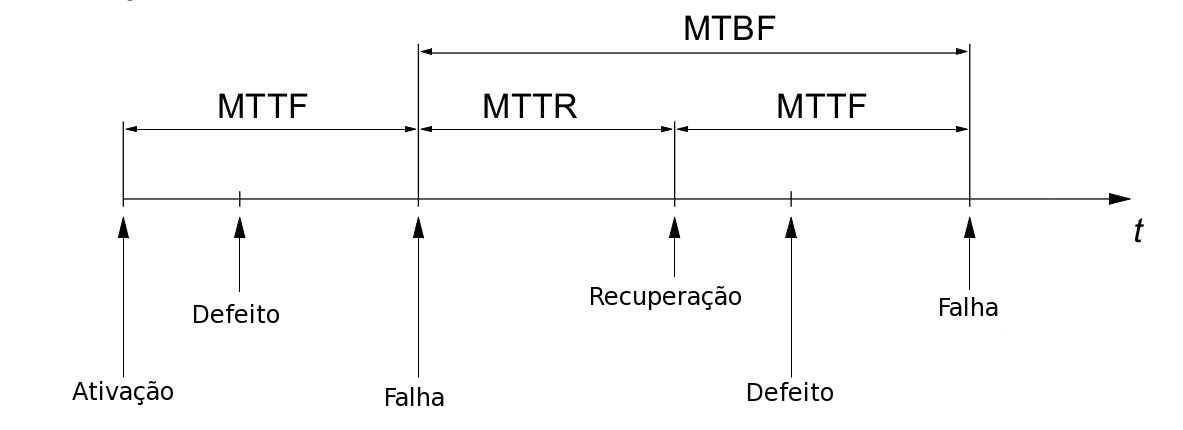
\includegraphics[width=1\textwidth]{images/grafico_mttf_mtbf}
\caption{Relação entre as falhas, defeitos, tempos médios de falha, tempos médios de recuperação e tempo médio entre falhas.}
\label{figure:grafico_MTTF_MTBF}
\end{figure}
Ao ser definida a probabilidade de um sistema operar conforme planejado até um instante de tempo $t$, está sendo definido o que se compreende por \textit{Confiabilidade}. Desta forma, a confiabilidade $R(t)$ de um sistema é normalmente descrita através de um expressão probabilística. Esta por sua vez considera que, para o período $t$ anteriormente mencionado, existe uma taxa de falha $\lambda$ que representa a probabilidade de falha deste sistema para um período $t$ \cite{Calabro1962}.

Na maioria dos casos, uma taxa de falha $\lambda$ constante é assumida \cite{Koren2007}, permitindo que a confiabilidade $R(t)$ seja expressada por uma função exponencial, explicitada na equação \ref{eq:Confiabilidade}.
\begin{equation} \label{eq:Confiabilidade}
R(t) = \textit{e}^{-\lambda t}
\end{equation}
Em concordância com definição de MTTF apresentada anteriormente, a mesma pode ser equacionada conforme mostrada na equação \ref{eq:MTTF}
\begin{equation} \label{eq:MTTF}
MTTF = \int_{0}^{\infty} R(t)dt = \frac{1}{\lambda}
\end{equation}

Para este trabalho o MTTF será empregado como a relação entre um acréscimo no atraso do circuito em uma saída especificada a priori, o acréscimo máximo permitido e o tempo de observação de envelhecimento do dispositivo. É importante salientar que  será abordada a falha $\lambda$ após o período de mortalidade infantil.
\subsection{Confiabilidade em Engenharia}
\label{subsection_Conf_Eng}
A confiabilidade em engenharia estabeleceu-se como um ramo de pesquisa nos tempos modernos, sendo o termo ``confiabilidade'' usado extensivamente pelo público em geral e pela comunidade técnica como sendo a capacidade de um sistema ou componente de operar normalmente sobre certas condições \cite{Maricau2013}. A base para a confiabilidade é a teoria probabilística e estatística, que permitiram o avanço deste campo de estudo tal como é conhecido atualmente. A partir daí, e com o advento da produção em massa de bens de consumo, o estudo da confiabilidade de sistemas se tornou essencial em projetos de engenharia, como foi o caso da (não)confiabilidade de tubos de vácuo \cite{Maricau2013}\cite{Saleh2006}.

Esta preocupação vital perdura até hoje, incluindo sistemas elétricos e eletrônicos de diferentes requisitos, e de forma pervasiva encontra-se em diferentes campos de estudo, tais como: sistemas de potência (modelagem baseada em agentes ou métodos clássicos) \cite{Endrenyi1979}\cite{Schlapfer}, rádio frequência \cite{Stephens2009}\cite{Larcher2006}, tempo de vida restante para transformadores de potência \cite{Osorio}–\cite{Jirutitijaroen2004}, sistemas de supervisão  e intervenção de estados clínicos \cite{LIMOUSIN1997}\cite{Arain2012}).

Os métodos e técnicas utilizadas são desenvolvidos, adaptados e/ou expandidos para esses diversos campos de pesquisa levando em consideração suas particularidades e quais fenômenos contribuem para o surgimento de falhas. Apesar destas particularidades, tais metodologias podem ser estudas em um âmbito mais generalista, sem prejuízo ao estudo de um problema específico \cite{Nelson2004}.

A confiabilidade de circuitos integrados tornou-se essencial para a indústria de CI's, sendo considerada um dos maiores problemas a ser enfrentado em curto prazo, como definido no ``The international technology roadmap for semiconductors''\cite{Hoefflinger2011}, explicitando efeitos como \textit{Time Dependent Dielectric Breakdown, Bias Temperature Instability} e \textit{Hot-Carrier Injection}.

\subsection{Técnicas de confiabilidade e robustez}
\label{subsection_Conf_tecnicas}
Diversas técnicas tem sido desenvolvidas e propostas para mitigar a redução de confiabilidade e robustez de sistemas. Tais técnicas podem abordar o problema diretamente na camada de \textit{hardware} ou de \textit{software}. Em adição, as abordagens pode ser divididas em dois grandes grupos \cite{Siewiorek1992}:
\begin{enumerate} 
\item \textbf{Intolerante à falhas:} Também conhecida como \textit{Prevenção de Falhas}, esta abordagem é considerada conservativa. A premissa neste caso é de que a redução da probabilidade de falha pode ser obtida através da utilização de dispositivos especialmente desenvolvidos para tal intento e/ou da utilização de métodos que propõe prolongar o tempo de vida do sistema;\item \textbf{Tolerante à falhas:} Já nesta abordagem as falhas são toleráveis pelo sistema. Estas técnicas se utilizam de redundâncias para, ou prover tempo extra para que o sistema volte à sua operação normal, ou garantir um caminho extra que, não submetido a uma falha, propague corretamente a informação desejada. 
\end{enumerate}

A seção \ref{subsubsection_tecnicas_hardware} irá sumarizar as propostas de algumas técnicas a nível de \textit{hardware} (\textit{i.e.} nível físico). Este trabalho apresentará posteriormente uma solução intolerante à falhas. É importante salientar que tais técnicas não são, necessariamente, mutuamente exclusivas.

\subsubsection{Técnicas em hardware}
\label{subsubsection_tecnicas_hardware}

De forma geral, as técnicas a nível físico podem ser distinguidas por \cite{Siewiorek1992}:
\begin{enumerate} 
\item \textbf{Modificação das condições ambientais:} engloba um conjunto de medidas que tendem a melhorar as condições ambientais de operação de um sistema, seja através da redução de efeitos degradantes de temperatura, dissipação de calor, radiação, entre outros;
\item \textbf{Melhoria de qualidade:} Neste caso é proposto a utilização de materiais com propriedades superiores ao já normalmente utilizados ou a melhoria da qualidade do processo de fabricação dos componentes que compõe o sistema;
\item \textbf{Duplicação:} é considerada uma técnica relativamente simples para detecção de falhas. Como o próprio nome indica, há uma duplicação de componentes e, havendo a falha em um destes, é feita uma comparação da informação. Uma diferença indica que uma falha ocorreu;
\item \textbf{Códigos para detecção de erros:} para estes casos, é averiguado qual conjunto de informações, de todas as possíveis em um sistema, realmente representa uma informação válida. Isso significa que para um conjunto de bits, por exemplo, apenas uma determinada combinação deles é esperada. A partir daí, uma comparação é realizada para determinar a validade dos dados. Aguns exemplos básicos desta técnica são os bits de paridade, códigos de Hamming e os \textit{checksums};
\item \textbf{Reconfiguração:} neste caso, após detectado o erro ou falha, o sistema altera parcialmente sua estrutura ou comportamento. Isso significa que ele pode combinar as técnicas anteriores, podendo rotear o caminho percorrido pela informação desejada para uma duplicata dos componentes que estão falhos, alterar o instante de sincronização das informações na saída ou até mesmo simplesmente desligar uma porção do sistema, fazendo com que ele opere de forma degradada.
\end{enumerate}


\subsection{Confiabilidade em circuitos integrados}
\label{subsection_Conf_CI}
Na década de 70, os problemas mais comuns de falha de dispositivos estavam relacionados à problemas de empacotamento e montagem (\textit{e.g.,} corros\~{a}o, conexão de fios e contaminação iônica). Somente após o advento de dispositivos integrados menores, efeitos como \textit{Hot Carrier Injection} se tornaram mais preocupantes, uma vez que começaram a afetar o desempenho destes dispositivos.

Encarados inicialmente como de f\'{a}cil prediç\~{a}o (\textit{i.e.,} determinísticos), tais efeitos passaram a ser considerados estocásticos e o primeiro deles a apresentar este comportamento foi o \textit{Time-Dependent Dielectric Breakdown} \cite{Solomon1977}. Estas mudanças surgiram \`{a} medida que a reduç\~{a}o do \'{o}xido do diel\'{e}trico se intensificou, atingindo a escala atômica. Com a continuada redução do tamanho dos dispositivos, entrando então na escala nanométrica, erros estocásticos e variações em nível atômico tornaram-se cada vez mais aparentes.

Variaç\~{o}es no processo de fabricaç\~{a}o surgem, introduzindo variabilidade nos dispositivos, e aumentando os desafios para projetistas de circuitos integrados.
Para este trabalho é importante compreendermos os fenômenos básicos através dos quais cargas ficam presas em determinadas regiões do transistor e como se relacionam com os mecanismos de envelhecimento que serão descritos em seguida. Tendo isto em mente, podemos então dividir os tipos de cargas nas seguintes categorias \cite{Leblebici1993}:
\begin{enumerate}
\item\textbf{Fixas no óxido}: proveniente de defeitos estruturais na camada de óxido que surgem durante processos de oxidação térmica, são encontradas próximas a interface $Si-SiO_2$. Esta região é normalmente descrita por $Si-SiO_x$, sendo uma representação intermediária entre o substrato e óxido. Assim sendo, são independentes das condições de operação do transistor;\item\textbf{Íons móveis no óxido}: são associados às impurezas no próprio óxido decorrentes dos processos de fabricação da estrutura \cite{Bentarzi2011};\item\textbf{Presas no óxido}: juntamente com as cargas presas na interface, tem um importante papel na degradação gradual das características do óxido. Estas cargas possuem energia cinética o suficiente para serem injetadas após vencerem a barreira de potencial da região entre o silício e óxido;\item\textbf{Presas na interface}: semelhantemente, estas cargas possuem uma energia cinética alta o suficiente para vencer a barreira de potencial porém não adentram o óxido, mantendo-se portanto na região interfacial entre o silício e óxido.
\begin{figure}[H]
\center
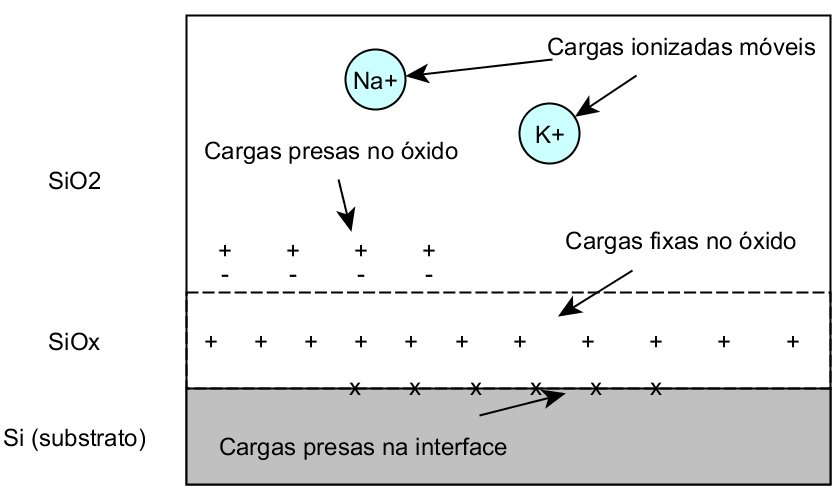
\includegraphics[width=0.5\textwidth]{images/armadilhas_interfaciais}
\caption{Tipos de cargas associadas a um estrutura $Si-SiO_2$.}
\label{figure:armadilhas_interfaciais}
\end{figure}
\end{enumerate}
Diversos modelos atômicos foram propostos para descrever as armadilhas que capturam elétrons e lacunas. A maioria destas armadilhas são usualmente ligações incompletas, como mostradas na figura \ref{figure:modelos_armadilhas}:
\begin{figure}[H]
\center
\subfloat[Interface sem imperfeições\label{figure:interface_perfeita}]{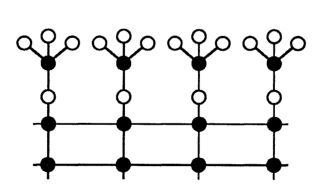
\includegraphics[width=0.4\textwidth]{images/interface_perfeita}}
\hfill
\subfloat[Interface com uma ligação incompleta,\label{figure:ligacao_incompleta_silicio}]{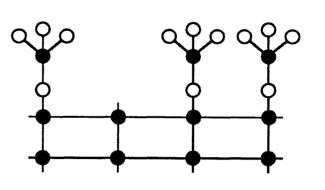
\includegraphics[width=0.4\textwidth]{images/ligacao_incompleta_silicio}}
\hfill
\subfloat[Interface com uma impureza,\label{figure:interface_impureza}]{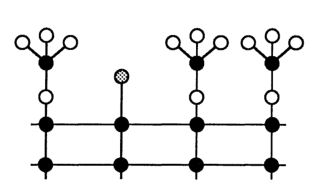
\includegraphics[width=0.4\textwidth]{images/interface_impureza}}
\hfill
\subfloat[Tipos de defeitos possíveis: ligação incompleta de silício e impureza no dióxido de silício\label{figure:tipos_impureza}]{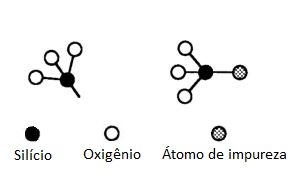
\includegraphics[width=0.4\textwidth]{images/tipos_impureza}}
\caption{Armadilhas para elétrons e lacunas em uma estrutura de $Si-SiO_2$ \cite{Leblebici1993}.}
\label{figure:modelos_armadilhas}
\end{figure}
\subsubsection{Hot Carrier Injection}
\label{subsection_HCI}
\textit{Hot Carrier Injection} (HCI) é um dos efeitos mais antigos e estudados, tendo sido introduzido por Shockley em 1961 para explicar fenômenos em junções \textit{p-n} à época \cite{Shockley1961}. O campo elétrico próximo à região de dreno de um transistor (e.g., \textit{MOSFET}) é considerado como a principal causa deste efeito, onde alguns portadores possuem uma energia cinética muito alta em comparação à média dos demais. Tais portadores de alta energia possuem uma temperatura efetiva acima da ambiente (``mais quentes'') e são capazes de vencer o potencial da superfície e são injetados no óxido de porta.

Parte destes portadores permanecem no óxido, gradualmente acumulando cargas e alterando a tensão de limiar $V_{TH}$ e a condutância $g_{o}$ ao longo da vida do dispositivo. Na década de 80 estes efeitos começaram a chamar a atenção, como consequência da redução contínua da escala dos transistores sem que existisse uma redução da tensão de alimentação \cite{Takeda1983}.

Já na década de 90, o \textit{HCI} foi mitigado com a redução da tensão de operação, redução esta que visava primeiramente um menor consumo de energia \cite{Maricau2013}. Entretanto, a variação da tensão não tem acompanhado a miniaturização \cite{Wang2007}\cite{Bravaix2009} dos dispositivos, não contribuindo significantemente com a redução desta degradação. Apesar de ser considerado menos relevante em dispositivos pMOS em comparação à dispositivos nMOS (pois as lacunas são mais pesadas que elétrons) o \textit{HCI} pode, ainda assim, realçar outros efeitos de envelhecimento \cite{Parthasarathy2006}. Atualmente quatro mecanismos de HCI são largamente conhecidos e estudados \cite{Maricau2013}:
\begin{enumerate}
\item \textbf{Channel Hot Electron (CHE):} Alguns elétrons ``sortudos'' (i.e., \textit{lucky electrons}), possuindo energia o suficiente, vencem a barreira da interface $Si/SiO_{2}$ na região do canal próxima ao dreno (ver figura \ref{figure:CHE_HCI}). Caso a tensão na porta $V_{g}$ seja baixa, o campo elétrico resultante não atrai suficientemente elétrons para a porta.   Quando a tensão  é aproximadamente igual à tensão do dreno $V_{d}$, atinge seu considerado valor máximo;
\item \textbf{Substrate Hot Electron (SHE):} Quando uma grande diferença de potencial é aplicada no corpo do transistor, seja positiva ou negativa, os portadores são direcionados para a interface $Si/SiO_{2}$ adquirindo energia cinética o suficiente para vencer a barreira ao longo de toda a interface do canal  e eventualmente sendo injetado no óxido de porta (ver figura \ref{figure:SHE_HCI}) uniformemente;
\item \textbf{Drain Avalanche Hot Carrier (DAHC):}  Em determinadas condições de estresse, onde a tensão $V_{d}$ no dreno é alta e a tensão $V_{g}$ é baixa, portadores de alta energia cinética podem colidir com elétrons, que antes estavam  ligados à estrutura cristalina, cedendo a eles energia, deixando-os livres para condução e criando um par elétron-lacuna no local \cite{Sze2007}. Estes, por sua vez, são acelerados mediante influência do campo elétrico no canal e podem potencialmente vencer a barreira da interface $Si/SiO_{2}$, ficando presos na região ou criando estados interfaciais (ver figura \ref{figure:DAHC_HCI}). Pode existir ainda uma componente adicional de corrente no corpo do transistor (i.e., \textit{bulk});
\item \textbf{Secondary Generated Hot Electron (SGHE):} esse efeito compreende a criação de portadores ``quentes'' (\textit{i.e.} hot carriers, HC) através da ionização por impacto envolvendo um segundo portador, sendo este também gerado por uma anterior ionização por impacto (e.g., \textit{DAHC}). Os primeiros portadores podem gerar durante seu deslocamento, por influência do campo transversal, novos portadores que, também acelerados por este campo em direção à interface, adquirem energia suficiente para a superar a barreira e atravessar o material (ver figura \ref{figure:SGHE_HCI}). Apesar disso, este efeito é considerado como um contribuinte inferior na degradação dos transistores se comparado aos demais efeitos \cite{Maricau2013}.
\end{enumerate}
\begin{figure}[H]
\center
\subfloat[CHE\label{figure:CHE_HCI}]{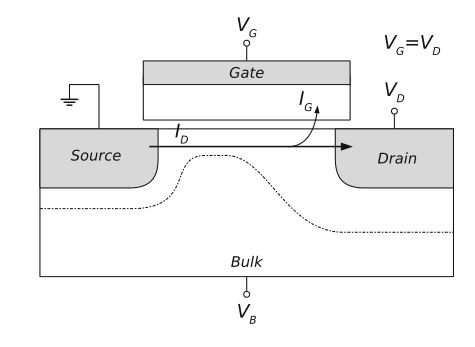
\includegraphics[width=0.45\textwidth]{images/CHE_HCI}}
\hfill
\subfloat[SHE\label{figure:SHE_HCI}]{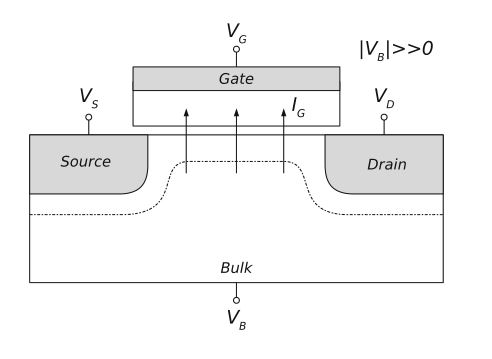
\includegraphics[width=0.45\textwidth]{images/SHE_HCI}}
\hfill
\subfloat[DAHC\label{figure:DAHC_HCI}]{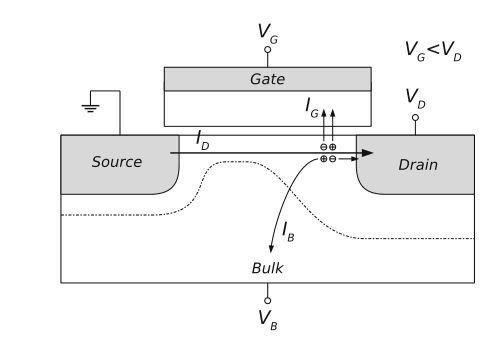
\includegraphics[width=0.45\textwidth]{images/DAHC_HCI}}
\hfill
\subfloat[SGHE\label{figure:SGHE_HCI}]{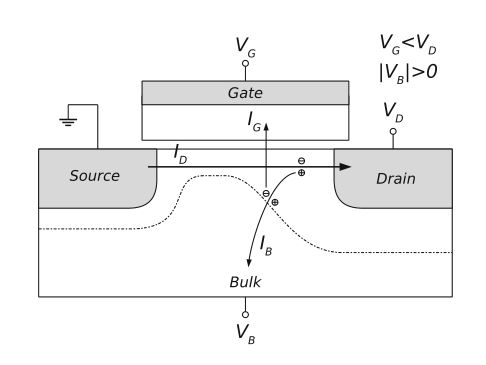
\includegraphics[width=0.45\textwidth]{images/SGHE_HCI}}
\caption{Mecanismos de injeção de portadores \cite{Maricau2013}.}
\label{figure:mecanismos_HCI}
\end{figure}
Estes quatro mecanismos se manifestam no transístor em diferentes condições de operação, sendo o DAHC e o CHE os que mais contribuem para a degradação do dispositivo. Para transistores de 0.35${\mu}$m, o DAHC é mais proeminente do que os demais efeitos. Já para dimensões inferiores, o CHE é considerado o efeito de degradação dominante \cite{Takeda1983}.
A variação na tensão de limiar através de HCI foi modelada como dependente do tempo, do campo elétrico no óxido $(E_{ox})$, do campo elétrico lateral máximo $(E_{lat})$, da temperatura $(T)$ e do comprimento do transistor $(L)$ :
\begin{equation} \label{eq:HCI1}
\Delta V_{TH} = A_{HCI}t^{n_{HCI}}
\end{equation}
sendo $A_{HCI}$ quantificado por \cite{Maricau2008}\cite{Kufluoglu}\cite{ChenmingHu1985}:
\begin{equation} \label{eq:HCI2}
A_{HCI} \propto \frac{1}{\sqrt{L}}exp \left(\alpha_{HCI,1}E_{ox}\right)exp\left(-\frac{\alpha_{HCI,2}}{E_{lat}}\right)
\end{equation}
onde $\alpha_{HCI,1}$ e $\alpha_{HCI,2}$ são parâmetros específicos da tecnologia.

\subsubsection{Bias Temperature Instability}
\label{subsection_BTI}
Conhecido de forma genérica por BTI (Bias Temperature Instability), é considerada uma das ameaças mais críticas em tecnologias CMOS. Apesar de conhecido há bastante tempo, este efeito tem se tornado mais proeminente em tecnologias abaixo de 90nm \cite{Amat2009}.

Este efeito é influenciado pela temperatura e se mostra presente quando uma tensão estressante é aplicada na porta do transistor, sendo percebido como uma alteração nos parâmetros de operação do transistor, tipicamente a tensão de limiar $V_{TH}$. No caso do NBTI, (\textit{i.e.} Negative BTI) esse fenômeno é observado em pFETs e em nFETs para o PBTI. Ainda n\~{a}o há um pleno consenso sobre a origem do BTI (a n\'{i}vel microsc\'{o}pico).

Alguns pesquisadores s\~{a}o de opini\~{a}o que este efeito surge de uma combinaç\~{a}o do aprisionamento de portadores nas imperfeiç\~{o}es do \'{o}xido e a geraç\~{a}o de estados na interface do canal do \'{o}xido.
Uma propriedade singular deste mecanismo se torna aparente em situaç\~{o}es nas quais s\~{a}o aplicadas tens\~{o}es estressantes sobre o dispositivo. Esta propriedade, conhecida como \textit{relaxamento} ou \textit{recuperaç\~{a}o}, indica a reduç\~{a}o da degradaç\~{a}o em um momento imediatamente posterior ao da apliaç\~{a}o da diferença de potencial estressante.

Por este motivo, a modelagem do BTI \'{e} complexa, com indícios de degradação residual após o relaxamento das condições de estresse, sendo indicados por duas componentes: uma permanente e outra recuperável \cite{Maricau2013}.
Alguns estudos modelam então este efeito como consequência de dois mecanismos \cite{Cho2010}:
\begin{enumerate}
\item
Geração de imperfeições próximas a interface entre silício e óxido, resultando numa componente de probabilidade de tunelamento dos átomos de Hidrogênio (H+);
\item E uma componente de recuperação, quantificando a captura e soltura de portadores.
\end{enumerate}
Este comportamento é matematicamente expresso da seguinte forma:
\begin{equation} \label{eq:BTI_permanent_recoverable}
\Delta V_{TH} \propto \left[ \underbrace{exp(\alpha_1 V_{GS})t^{n_P}}_{\text{Componente permanente}} + \underbrace{V_{GS}^{\alpha_2}(C_R + n_R \log_{10}({t}))}_{\text{Componente recuperável}} \right] exp\left(-\frac{E_a}{kT}\right)
\end{equation}

sendo a variação da tensão de limiar, $\Delta V_{TH}$, uma função do campo elétrico $(E_{ox})$ aplicado no óxido de porta do transistor e a temperatura $(T)$. Os parâmetros $\alpha_1$ e $\alpha_2$ são fatores de escalonamento da voltagem e dependentes da tecnologia empregada, $E_a$ é a energia de ativação correspondente, $C_R$, $n_P$ e $n_R$ são expoentes de ajuste do tempo para as componentes permanente e recuperável, e $k$ é a constante de Boltzman.

É importante salientar que a equação \ref{eq:BTI_permanent_recoverable} só é válida para uma voltagem estressante que seja invariante, sendo necessária um modelo mais preciso para o BTI quando a tensão aplicada é variante no tempo \cite{Grasser2009a}.
Os efeitos de BTI s\~{a}o considerados determin\'{i}sticos para transistores de tamanho microm\'{e}trico, com uma variaç\~{a}o id\^{e}ntica nos par\^{a}metros dos transistores \cite{Wang2007}.

Porém, ao serem reduzidos para a escala nanométrica, estes efeitos passam a ser considerados como estocásticos. A mudança dos parâmetros dos transistores varia com o tempo. Além disso, estas mudanças são intensificadas pelo aumento do desvio padrão deste mesmos parâmetros, também no tempo. 
\subsubsection{Time-Dependent Dieletric Breakdown}
\label{subsection_TDDB}
A operação adequada de um transistor MOS exige que o mesmo esteja operando sob as corretas condições, incluindo aí a magnitude do campo elétrico aplicado na sua região isolante. Estes campos elétricos podem eventualmente exceder o campo elétrico máximo suportado pelo dielétrico e levá-los à ruptura. Como consequência há um acréscimo substancial da corrente na porta deste transistor.

Mas mesmo durante a operação normal de transistores, diferentes estados de ruptura podem se manifestar, sendo importante diferenciar as categorias existentes e em quais condições elas podem surgir, quais sejam \cite{Maricau2013}:
\begin{enumerate}
\item \textbf{Soft breakdown (SBD)}: é observada como uma perda parcial das propriedades dielétricas, em comparação com o \textit{Hard Breakdown}, e que n\~{a}o impede a operaç\~{a}o do mesmo. Apesar disso, o dispositivo passa a operar em condiç\~{o}es n\~{a}o idealizadas pela sua especificaç\~{a}o. Entretanto possuem apenas um pequeno aumento da corrente de porta e a completa quebra do dispositivo é improvável \cite{Maricau2013};
\item \textbf{Progressive breakdown (PBD)}: É um passo gradativo que surge após o SBD, sendo percebido como um pequeno incremento na corrente de porta no decorrer do tempo. É presenciado em estruturas de óxido ultra-fino, tipicamente abaixo de 2.5nm de espessura;
\item \textbf{Hard breakdowns (HBD)}: é percebida como um aumento significativo da corrente de porta e uma redução da controlabilidade da tensão de porta do dispositivo. Este tipo de ruptura em qualquer transistor é considerada como sendo capaz de causar uma falha permanente no circuito.
\end{enumerate}
O TTDB é entendido como sendo este processo de danificação gradual no óxido graças a estes fortes campos elétricos.
Apesar da importância do TDDB para o estudo da confiabilidade de transistores, os modelos f\'{i}sicos a n\'{i}vel molecular existentes são, de certa forma, especulativos \cite{McPherson2012}, divindo-se em tr\^{e} categorias principais: \textit{a)} modelamento pelo campo el\'{e}trico; \textit{b)} modelamento pela corrente el\'{e}trica; \textit{c)} e modelamento pela combinação de ambos. Apesar de não existir um modelo largamente aceito, existem algumas características que são amplamente reconhecidas \cite{McPherson2012}:
\begin{enumerate}
\item TDDB é fortemente dependente do campo;
\item TDDB pode ser fortemente dependente da temperatura;
\item TDDB pode ser dependente da polaridade;
\item Alguns defeitos, armadilhas e ligações incompletas podem ser formadas durante o estresse causado por TDDB;
\item A geração de falhas leva a criação de um caminho condutivo de infiltração que, eventualmente, ocasiona a quebra do dispositivo;
\item O TDDB pode ser estatisticamente descrito por distribuições de Weibull;
\item Os parâmetros de aceleração de partículas no campo crescem diretamente proporcional à constante dielétrica $\kappa$.
\end{enumerate}
Assim sendo, o entendimento do mecanismo por detr\'{a}s da quebra do diel\'{e}trico é de vital importância. Os defeitos gerados durante o estresse são normalmente consideradas como neutros pois não há mudança significativa do diagrama de banda de energia para um disposotivo MOS. Al\'{e}m disso, acredita-se que estes defeitos devem estar relacionados a um processo de geração de defeitos a nível molecular \cite{McPherson2012}. Ainda mais: a geraç\~{a}o de defeitos no material \'{e} considerada irrevers\'{i}vel.

Mesmo ap\'{o}s o recozimento do dispositivo ou a invers\~{a}o do campo, n\~{a}o há evid\^{e}ncia de um aumento significativo do tempo de vida. O entendimento passa a ser de que o dano causado permanece na rede de silício e é praticamente irreversível. Este tipo de comportamento é então associado à mudanças na ligação dos átomos. Durante a ruptura da ligação covalente do íon de silício, por influência do campo elétrico local, há a criação de ligações incompletas (\textit{i.e.} dangling bonds) que possuem apenas um elétron e de uma estrutura diferente (ver figura \ref{figure:mecanismos_TDDB_vacancies}).
\begin{figure}[H]
\center
\subfloat[Orientação tetraédrica da ligação Si-Si.\label{figure:TDDB_SiSi_tetra}]{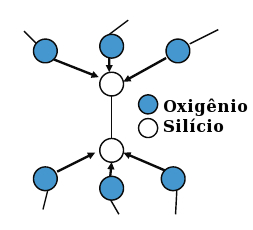
\includegraphics[width=0.45\textwidth]{images/TDDB_vacancies_a}
}
\hfill
\subfloat[A estrutura da rede é alterada após a quebra da ligação Si-Si e sofre forte influência de um campo $E_{loc}$ local àquela ligação incompleta. \label{figure:TDDB_SiSi_tri}]{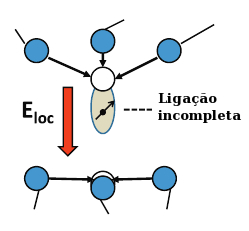
\includegraphics[width=0.45\textwidth]{images/TDDB_vacancies_b}
}
\caption{Geração de ligações incompletas a partir de vacâncias \cite{McPherson2012}.}
\label{figure:mecanismos_TDDB_vacancies}
\end{figure}
Esta estrutura pode ser ``relaxada'' a tal ponto que mesmo após o recozimento ou alteração do sentido do campo, como mencionado anteriormente, a ligação não será reparada, sendo esta uma das observações mais significantes do estresse provocado pelo TDDB.

Diversos modelos têm sido propostos para as categoria anteriormente mencionadas. Para o \textit{HDB}, os mais conhecidos são: modelo termoquímico (\textit{i.e.} termochemical), modelo injeção-anodo-lacuna (\textit{i.e.} anode-hole-injection) e o modelo direcionado à voltagem (\textit{i.e.} voltage-driven).
O modelo termoquímico é conhecido como \textit{modelo} $E$ (\textit{i.e.} E model), pois considera que existe uma correlação direta entre o campo elétrico aplicado no óxido do dispositivo $E_{ox}$ e o tempo de vida do dispositivo; sendo as ligações químicas no óxido fracas o suficiente para que este campo elétrico as rompa.

Assim sendo, o tempo para quebra (\textit{i.e.} time to breakdown) $t_{BD}$ é expresso por \cite{McPherson1985}:
\begin{equation} \label{eq:TDDB_time_to_break_Emodel}
t_{BD}\propto \exp\left(-\gamma E_{ox}\right)\exp\left(\frac{E_{a}}{kT} \right)
\end{equation}
onde $\gamma$ ($\gamma\approx$ 1.1década/MV/cm) é um fator de aceleração do campo e $E_a$ ($E_a\approx 0.6 - 0.9$eV) é a energia de ativação térmica.

Já o modelo injeção-anodo-lacuna é conhecido como \textit{modelo} $1/E$ e prevê uma dependência entre o $t_{DB}$ e o campo elétrico, sendo uma consequência da captura de lacunas em determinadas regiões do óxido de porta. Ela é expressa por \cite{ChenmingHu1985}:

\begin{equation} \label{eq:TDDB_time_to_break_1/Emodel}
t_{BD}\propto \exp\left(\frac{\beta}{E_{ox}}\right)\exp\left(\frac{E_{a}}{kT} \right)
\end{equation}
onde $\beta$ ($\beta\approx$ 350MV/cm) é um fator de aceleração do campo dependente do processo de fabricação.
Existem ainda modelos que combinam os dois propostos acima. De todo caso, estes modelos vem sendo revisados para óxidos de porta inferiores à 5nm \cite{Maricau2013}.
Na seção \ref{subsubsection_Modelos_TDDB} serão apresentados modelos mais precisos e modernos.

\subsection{Estado da arte}
\label{subsection_estado_da_arte}
As diversas técnicas de confiabilidade de circuitos integrados utilizadas para reduzir o impacto do envelhecimento se concentram em contramedidas tais como: blindagem de circuitos, faixas de segurança (\textit{i.e.} guard-banding), balanceamento de cargas, voltagem dinâmica e escalonamento de frequência \cite{Mintarno2010}\cite{Mitra2011}, se encaixando em uma outra das categorias definidas na seção \ref{subsubsection_tecnicas_hardware}.

Para suportar algumas destas estratégias deve-se prever a falha de um sistema com antecedência, usando tal informação para ajudar na tomada de decisões destas contramedidas antes mesmo que qualquer erro se manifeste. Esta estratégia se diferencia da abordagem clássica, que atua somente após o surgimento de erros. Uma abordagem que vêm sendo explorada é a de utilização de sensores variados em diversos locais do sistema, coletando informações sobre diversos parâmetros de operação ao longo do tempo. 

Eles podem ser analisados internamente ou externamente na procura de anomalias que indiquem que o sistema irá falhar. A frequência desta coleta pode ser ajustada a nível de design ou ser adaptativa durante a operação, permitindo que esta frequência seja adequada ao longo da operação para melhor capturar comportamentos que sejam anômalos ou que levem a uma degradação do sistema \cite{Agarwal2007}. Exemplos de dados a serem coletados são: temperatura, tensão de alimentação, atrasos, grau de atividades e outros que o projetista julgar importante.

Estes sensores podem ser \textit{in-situ}, adicionados a caminhos críticos específicos para detectar o não cumprimento de restrições de tempo; \textit{online self-testing}, onde um sistema entra em modo de teste e executa rotinas de \textit{Built-On Self Test} (BIST) que auxiliam na determinação da degradação corrente; \textit{sensores de envelhecimento}, que utilizam circuitos de referência espalhados pelo sistema que informam alteração em parâmetros de operação; e \textit{monitores de estresse}, que coletam informações de temperatura, alimentação e carga do sistema.

Técnicas como \textit{shadow transistors} incluem transistores paralelos entre aqueles que, previamente identificados, são considerados mais vulneráveis. Desta forma, não apenas o tempo de vida é melhorado como também são compensadas as falhas inseridas durante a fase de fabricação (\textit{e.g. circuitos abertos}). Esta medida não reduz a taxa de falha $\lambda$ de um determinado transistor mas inclui um caminho adicional em sua \textit{netlist}, reduzindo a probabilidade de falha, já que ambos os caminhos, tanto o original como a duplicata, devem falhar para que haja o sistema falhe \cite{Cornelius2008}.

Esta técnica pode ser realizada através da inserção guiada ou aleatória de \textit{shadow transistors}, conduzindo a resultados promissores. A técnica pode ser combinada com transistores de espessuras de óxido diferentes, aumentando ainda mais a confiabilidade de um sistema. Entretanto, tais técnicas têm como consequência o aumento da área, acréscimo do consumo dinâmico e do atraso médios.

Outra forma de aumentar a confiabilidade de um sistema é através da utilização de \textit{sleep transistors}. Estes transistores de alta tensão de limiar $V_{TH}$, sejam pMOS ou nMOS, são utilizados para interromper a alimentação de partes do sistema que eventualmente esteja em modo de espera. Entretanto, esta técnica necessita considerar diversos aspectos, tais como: ativação por nMOS ou pMOS, qual será a distribuição espacial dos \textit{sleep transistors}, largura e profundidade da porta, otimização área ocupada pelo corpo do transistor, fugas e eficiência \cite{Shi}.

Esses, por sua vez, podem ser utilizados para alternar a ativação de módulos do sistema. Ao desconectar a alimentação de um módulo ele não irá, idealmente, apresentar tensões ou correntes e consequentemente nenhum campo elétrico. A consequência é uma redução da temperatura e ausência de atividade. Isto é importante na redução de efeitos indesejados, tais como: eletromigração \cite{Srinivasan2003}, ruptura do óxido de porta e NBTI.

Então, durante a fase ociosa das portas este efeitos serão eliminados ou reduzidos drasticamente. Como consequência desejada, o MTTF é prolongado \cite{Torres2013}. Esta técnica é conhecida como \textit{Alternating Module Activation} (AMA).

Em abordagens mais recentes, a melhoria da confiabilidade de um sistema está sendo obtida através da adoção de técnicas de aprendizado de máquina (\textit{i.e.} machine learning) que permitem representar e prever qual é a degradação que um sistema sofre através da observação de caminhos críticos. Ao observar por um período de tempo $t$ qual é o acréscimo no atraso das saídas destes caminhos, estas informações são relacionadas à carga de trabalho a qual o sistema está submetido. Esta carga e este tempo $t$ são determinados durante o design e a predição é \textit{online}.

Tais informações de design (tempo de observação, caminhos críticos e saídas observáveis) são decididas pelo projetista e alteram a precisão da predição \textit{online}. Porém, durante a operação, as informações utilizadas pelo modelo podem ser atualizadas à conveniência do projetista. Esta decisão impacta a área ocupada pelo sistema, pois acarretará na inclusão de dispositivos à estrutura, tornando-a maior. Parte desta tarefa de monitoramento e predição pode ser dividida entre componentes de hardware e software, mitigando uma porção deste acréscimo de área e permitindo a integração de modelos mais complexos.

Trabalhos realizados nesta área relatam que esta estratégia apresenta uma boa precisão e é considerada promissora \cite{Baranowski2015}. Entretanto, estes trabalhos consideram somente alguns dos fenômenos de envelhecimento, tais como NBTI, e apenas parte das condições ambientais que contribuem para o envelhecimento de transistores (\textit{e.g.} temperatura, tensão de alimentação e atividade).

Essas diversas abordagens endereçam o mesmo problema mas sugerem ações diferentes, porém complementares. Isto é importante pois permite que tecnologias mais robustas de verificação, avaliação e relatórios se tornem viáveis. Ao atuarem em diversas camadas de abstração, que têm se tornado cada vez mais complexas, novas tecnologias podem integrar essas soluções, mitigando ou corrigindo erros e falhas nessas diferentes camadas. Assim sendo, a confiabilidade de um sistema é melhorada como um todo.

Em \cite{Maeda2014} temos um exemplo da empregabilidade de tais abordagens em uma tecnologia que, sendo uma proposta universal, integra e arbitra a comunicação entre estes elementos. 

\subsection{Modelos Compactos}
\label{subsection_modelos_compactos}

Na seção \ref{subsection_Conf_CI} foram apresentados os principais efeitos físicos responsáveis pelo envelhecimento de circuitos integrados. Foram apresentados ainda alguns modelos que se propõem a explicar as relações entre os parâmetros de operação e as degradações observadas. Esta seção discute o desenvolvimento de modelos compactos para transistores MOS.

Será discutido primeiramente os modelos existentes para HCI e em seguida para um enfoque nos modelos existentes para baias temperature instability e TDDB.
	
\subsubsection{Modelos para HCI}
\label{subsubsection_Modelos_HCI}

Considerado no início como um efeito de grande importância para explicar a degradação de transistores, o HCI se tornou um efeito menos dominante à medida que a tensão de alimentação foi sendo reduzida. Entretanto ele ainda é considerado um problema para tecnologias atuais visto que o campo elétrico vem aumentando gradativamente com a redução do tamanho dos transistores.

Diversos modelos foram publicados ao longo dos anos para explicar o HCI.  Entre eles o modelo do elétron ``sortudo'' (\textit{i.e. lucky electron model}, LEM) é um dos mais conhecidos. Além disso, muito dos outros modelos que surgem posteriormente são derivados do LEM. Em 1985 \cite{ChenmingHu1985} foi um dos primeiros a introduzir o modelo baseado no LEM. As propostas que se seguem utilizam a mesmo teoria mas propõem uma formulação analítica diferente ou propõem uma acomodação do modelo para tecnologias CMOS mais avançadas.

No trabalho apresentado em \cite{Kufluoglu} os efeitos de HCI e NBTI foram unificados em um mesmo modelo, levando em consideração a geração de armadilhas interfaciais devido a desassociação das ligações de Si-H. Posteriormente esta proposta é utilizada para desenvolver outros modelos para tecnologias mais avançadas. Um modelo semi-empírico foi proposto e pode ser expressado de acordo com a quantidade de estados interfaciais gerados:
\begin{equation}\label{eq:HCI_semi_empircal_states}
\Delta N_{IT}=C_1\left[\frac{I_{DS}}{W}\exp\left(-\frac{\phi_{IT,e}}{q\lambda_eE_{lat}}\right)T_{str}\right]^n
\end{equation}
onde $W$ é a largura de canal do transistor, $I_{DS}$ é corrente dreno-fonte, $E_{lat}$ é o campo elétrico lateral máximo no dreno, $T_{str}$ é o tempo de estresse ao qual o transistor é submetido, $\phi_{IT,e}$ é a energia crítica necessária para que os elétrons criem uma armadilha interfacial \cite{Maricau2013}. 

Apesar desses modelos serão baseados no LEM, eles incluíam apenas uma fonte de portadores ``quentes''. Entretanto, como mostrado anteriormente na seção \ref{subsection_HCI}, existem outros três mecanismos que foram identificados ao longo dos anos de pesquisa e que podem potencialmente resultar em uma mudança no comportamento do transistor ao longo do tempo.

Posteriormente, \cite{Maricau2013} propôs um modelo baseado em uma abordagem conhecida como reação-difusão (\textit{i.e. reaction-diffusion}, RD) proposta em \cite{Kufluoglu} e também baseado no LEM. O modelo RD possui alguns pontos negativos ao tentar modelar o BTI. Um desses é a incapacidade de considerar o aprisionamento de óxidos.

Entretanto esse efeito está relacionado ao fenômeno de recuperação do BTI, que ocorre após o estresse aplicado no dispositivo cessar. Entretanto, esse modelo ainda pode ser utilizado para modelar o efeito de HC, visto que as armadilhas interfaciais são geradas próximas ao fim da região do dreno, onde efeito de recuperação é negligenciável.

É utilizado então um conjunto de duas equações diferenciais que descrevem a geração das partículas de hidrogênio próximas à interface óxido canal e qual é a sua difusão em direção ao contato da porta. Essas equações são então resolvidas numericamente ao sinalizar um transistor. Porém essa análise não é apropriada para o estudo de um circuito inteiro.

Em \cite{Maricau2013}, é proposta uma expansão deste modelo, válido somente para tensões de estresse contínuas (modelo DC). Entretanto circuitos integrados atuais são submetidos a tensões que variam no tempo. Para incluir essa variação uma extensão ao modelo DC deve ser incluída, um modelo AC. 

Ainda em \cite{Maricau2013}, ambos os modelos, AC e DC, são combinados para avaliar o impacto do HCI no comportamento do transistor graças à sinais estressantes variantes no tempo.

\subsubsection{Modelos para BTI}
\label{subsubsection_Modelos_BTI}

Para  transistores cuja tecnologia está abaixo de 90 nanômetros, o NBTI é considerado uma das maiores ameaças a confiabilidade de dispositivos. Assim sendo, é considerado essencial prever quais são os impactos desse efeito na performance de circuitos integrados. Apesar de também presente, o PBTI recebe um enfoque menor.

Um dos principais desafios enfrentados ao se analisar este efeito é explicar o comportamento dele a nível microscópico. Na década de 70, algumas pesquisas já sugeriam que a criação de estados na interface estava relacionada ao mecanismo de difusão do hidrogênio. Esse mecanismo foi posteriormente chamado de reação-difusão (RD). Em 2006 foi sugerido que o NBTI consiste de uma geração de estados na interface mais ou menos constante combinada a um componente de recuperação relacionada ao aprisionamento de lacunas \cite{Parthasarathy2006}.
\\

\textbf{Modelo de Reação-Difusão}

Este modelo propõe que uma reação ativada termicamente entre lacunas e ligações de Si-H na interface dielétrico/substrato do MOSFET resulta na geração de ligações incompletas. Estas por sua vez levam ao surgimento de estados interfacias. As partículas de hidrogênio se afastam da interface por difusão e vão em direção ao dielétrico de porta.

O modelo mais conhecido foi proposto em \cite{Alam2003} e posteriormente aperfeiçoado por outras pesquisas \cite{Schroder2003}\cite{Chakravarthi2004}. De acordo com o modelo RD. Esta reação eletroquímica é então definida como depende da temperatura e do campo; e a taxa da geração de armadilhas é descrita pela seguinte equação diferencial:
\begin{equation}\label{eq:BTI_RD_diff}
\frac{d N_{IT}}{dt} = k_F\left(N_0 - N_{IT}\right) - k_RN_H(0)N_{IT}
\end{equation}
sendo $N_{IT}$ uma variável para representar a quantidade de armadilhas interfaciais, $N_0$ é a quantidade inicial de ligações incompletas de Si-H e $k_F$ é uma constante que representa a taxa de desassociação depende do campo no óxido. $k_R$ é a taxa de recozimento das ligações incompletas associada aos átomos de hidrogênio. $N_H(0)$ é a concentração de hidrogênio na interface. Entretanto, os átomos de hidrogênio podem difundir da interface para dentro do óxido, sendo este processo descrito por:
\begin{equation}\label{eq:BTI_RD_hydrogen_diff}
\frac{d N_{H}}{dt} = D_H\frac{d^2N_H}{dx^2}
\end{equation}
onde $N_H$ é a concentração total de hidrogênio no óxido e $D_H$ é uma constante de difusão. Estas ligações incompletas atuam como armadilhas ``doadoras'' que contribuem para variação na tensão de limiar $V_{TH}$, que pode ser representada por:
\begin{equation}
\Delta V_{TH}=\frac{qN_{IT}}{C_{ok}}
\end{equation}
sendo $q$ a carga de um elétron e $C_{ox}$ a capacitância do óxido de porta.

A figura \ref{figure:RD_model} mostra de forma simplificada onde estes fenômenos ocorrem.
\begin{figure}
\center
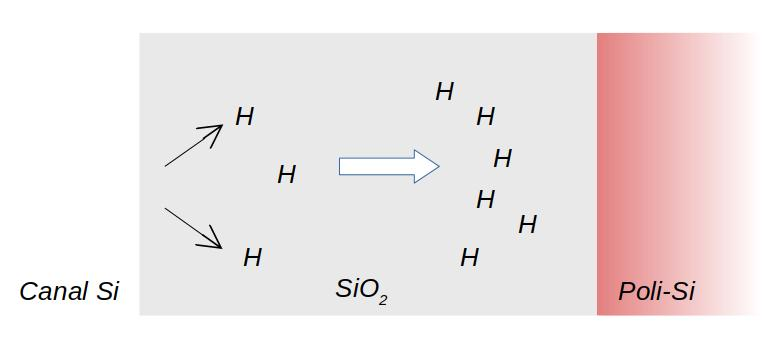
\includegraphics[width=0.5\textwidth]{images/RD_model}
\caption{Representação da quebra de ligações Si-H e Si-O na interface $Si/SiO_2$}
\label{figure:RD_model}
\end{figure}
\subsubsection{TDDB}
\label{subsubsection_Modelos_TDDB}

Como explicado anteriormente na seção \ref{subsection_TDDB}, a quebra do óxido de porta pode se dar em etapas, indo de um Soft Breakdown (SBD) a um Hard Breakdown (HBD); sendo necessário então descrever quais mecanismos estão envolvidos nestas duas etapas e como podemos modelar tal comportamento.
\\

\textbf{Modelo para Hard Breakdown}

Existem diversos modelos que se propõe a explicar este fenômeno, sendo um dos mais conhecidos o modelo \textit{termoquímico}. Entretanto ele foi gradativamente modificado para atender a resultados obtidos em experimentos posteriores, que indicavam que as formulações descritas nas equações \ref{eq:TDDB_time_to_break_Emodel} e \ref{eq:TDDB_time_to_break_1/Emodel} não eram mais válidas para óxidos de porta com espessuras menores do que 5nm \cite{Wu2001}.

O modelo foi expandido posteriormente para incluir a dependência da área e a distribuição do \textit{tempo para ruptura} \cite{Wu2005}, visto que anteriormente só era prevista o tempo para quebra característico. Entretanto, alguns dispositivos falhavam antes desse tempo.

Considerando estas mudanças, um modelo completo para tempo de quebra em óxidos ultrafinos (\textit{i.e.} $t_{ok} < 5nm$) pode ser descrito por:
\begin{equation}\label{eq:TDDB_complete_model}
t_{BD}\propto \left(\frac{1}{WL}\right)^{1/ \beta}F_{BD}^{1/\beta}V_{GS}^{a+bT}\exp\left(\frac{c}{T} + \frac{d}{T^2}\right)
\end{equation}
sendo $W$ e $L$ a largura e o tamanho do transistor, respectivamente. As contantes $\beta$, $a$, $b$, $c$ e $d$ são dependentes da dimensão do transistor CMOS \cite{Li2008}.

O tempo de quebra segue uma distribuição de Weibull e sua função de probabilidade de falha cumulativa $F_{BD}$ é descrita por:
\begin{equation}\label{eq:TDDB_probability_function}
F_{BD}=1-\exp \left(-\frac{t}{t_{BD,63}}\right)^\beta
\end{equation}

\textbf{Modelo para Soft Breakdown}

Passando a ser importante com o advento de dielétricos ultrafinos, o SBD não se traduz na perda de controlabilidade da tensão de porta do transistor mas sim em um pequeno acréscimo da corrente de porta e na criação de um caminho de infiltração no óxido. Porém, assim como o HBD, o SBD também segue uma distribuição de Weibull.

Essa infiltração no óxido é gradual e em concordância com o pequeno incremento da corrente de porta encontrado experimentalmente \cite{Sahhaf2009}. Isso significa também que um único ponto de infiltração tem uma baixíssima probabilidade de impedir o funcionamento de um circuito. Porém um conjunto deles ao longo do tempo aumenta essa chance, sendo necessário modelar a quantidade de pontos de infiltração após um período de estresse.

A probabilidade de existirem $n$ defeitos de SBD em um instante de tempo $\chi$ pode ser descrita por uma distribuição de Poisson \cite{Wu2005}:
\begin{equation}
P_n(t)=\frac{\chi^n}{n!}\exp(-\chi)
\end{equation}
\begin{equation}
\chi = \left(\frac{t}{t_SBD,63} \right)^\beta
\end{equation}
\begin{equation}
t_{SBD,63} = t_{SBD,ref} \left(\frac{WL}{A_{ref}}\right)^{1/\beta}\left(\frac{V_{GS}}{V_{ref}}\right)^\gamma
\end{equation}
onde $t_{SBD,63}$ está associado ao tempo de quebra no 63º percentil para um transistor de referência de área $A_{ref}$ estressado a uma tensão $V_{ref}$. $\beta$ e $\gamma$ são parâmetros dependentes do processo do transistor \cite{Sahhaf2009}.

Este modelo entretanto não é dinâmico, pois não considera mudanças na tensão de estresse aplicada, mudanças estas que são consequência da alteração dos parâmetros de operação do transistor; e esta alteração é induzida justamente pelo envelhecimento.

Em \cite{Maricau2013} o modelo é alterado para considerar este dinamismo e descrever a probabilidade $P_n(t_2)$ de encontrar $n$ pontos de SBD em um instante de tempo $t_2$. Ela está relacionada à probabilidade $P_n'(t_1)$ de encontrar n' pontos de SBD no instante de tempo $t_1$:
\begin{equation}
P_n(t_2)=\sum_{n'=0}^{\infty}\left[P_{n'}(t_1)\frac{\Delta \chi^{n-n'}}{(n-n')!}\exp(-\Delta\chi) \right]
\end{equation}
\begin{equation}
\Delta\chi = \left(\frac{t_2-t_1}{t_{SBD|V_{GS1}=V{GS2}}} \right)^\beta
\end{equation}
sendo $V_{GS1}$ a tensão de estresse em $t_1$ e $V_{GS2}$ em $t_2$.
\subsection{Simuladores}
\label{subsection_Simuladores}

Com os efeitos de envelhecimento de transistores possuindo um impacto cada vez maior, a simulação da confiabilidade de circuitos eletrônicos se tornou uma parte importante em um fluxo moderno de design. Simulações precisas da confiabilidade permitem que o projetista aumente significantemente o design, satisfaça especificações mais complexas e ainda assim garanta uma operação confiável do sistema.

Diversas ferramentas surgiram na década de 70 após o advento do simulador \textit{SPICE}. Apartir daí, a complexidade das ferramentas seguiu o avanço dos métodos utilizados para caracterizar o envelhecimento de transistores e são construídos ao redor do \textit{SPICE} \cite{Maricau2013}.

Este trabalho utiliza o simulador Relxpert$^{\copyright}$ (Cadence Systems$^{\copyright}$), baseado no \textit{BERT\copyright}, que fornece um modelo analítico descrevendo cada efeito de envelhecimento. Normalmente, os modelos devem ser fornecidos pelos fabricantes, mas podem ser desenvolvidos pelo próprio pesquisador. Esses modelos devem descrever as mudanças nos parâmetros dos dispositivos como função da idade do transistor. Apesar de utilizar esta ferramenta, a metodologia que será apresentada independente da escolha feita pelo pesquisador.


% ----------------------------------------------------------
% Related Works
% ----------------------------------------------------------
% Não mais necessário
% \chapter{Trabalhos relacionados}


% ----------------------------------------------------------
% ----------------------------------------------------------
% Methodologies used on this work
% ----------------------------------------------------------
\chapter{Metodologia}
\epigraph{\textit{How do you know but ev’ry Bird that cuts the airy way, Is an immense world of delight, clos’d by your senses five?}}{-William Blake}
\section{Motivação}
Como exposto anteriormente na seção \ref{subsection_Conf_Eng}, a confiabilidade de um sistema pode ser quantificada por seu MTTF. Existem diversos fatores que podem afetá-lo e estes podem se manifestar em diversas fases da concepção e operação de um sistema: na variação do processo de fabricação, no design, durante a interação com fatores externos estranhos ao sistema (\textit{p.ex.} descargas elétricas, radiação).

Desta forma, diversos métodos e técnicas são viáveis para mitigar a degradação de transistores nestas fases, combinados ou não. Entretanto, todas estas abordagens alteram, eventualmente, a tensão de operação, a atividade do sistema e indiretamente a temperatura.

Partindo dessa premissa, este trabalho se propõe a averiguar como os parâmetros de tensão e temperatura estão variando ao longo da operação do sistema e investigar a relação destes com a degradação.

\section{Visão geral}
\label{section_visao_geral}
Neste trabalho, os dados de condições ambientais (\textit{p.ex.} tensão e temperatura) auxiliam na criação de um \textit{perfil de operação} para um sistema observado ao longo do tempo. Esse perfil é representado por um conjunto de variações das condições ambientais que, empregadas sobre os dispositivos, contribuem para a degradação e, consequentemente, envelhecimento dos mesmos. Isso nos permite associar de forma única esse perfil a um MTTF.

O MTTF pode ser associado a diferentes eventos dentro do ciclo de vida de um sistema, tais como: tempo médio até o surgimento de falhas permanentes em porções especificas dos circuitos, falhas transitórias e intermitentes, tempo necessário até a falha completa ou parcial de um sistema. Neste trabalho, o MTTF é considerado como sendo o tempo necessário para que um sistema sofra uma degradação alta o suficiente que o force a violar suas especificações de projeto. Em outras palavras, os circuitos não são mais capazes de cumprir suas especificações de temporização.

A partir disso, o \textit{Tempo de Vida Restante} (\textit{i.e. Remaing Useful Lifetime, RUL}) é definido como o tempo remanescente do sistema durante o qual ainda funcionará, antes de falhar \cite{Urmanov2007}. O RUL é, usualmente, determinado pela diferença entre seu tempo de vida atual e seu MTTF. Ao assumir esta proposição, a predição do MTTF através da observação da variação de temperatura $T$, tensão de operação $V$ e da atividade $\alpha$ permite predizer também o RUL.

\begin{figure}[H]
	\center
	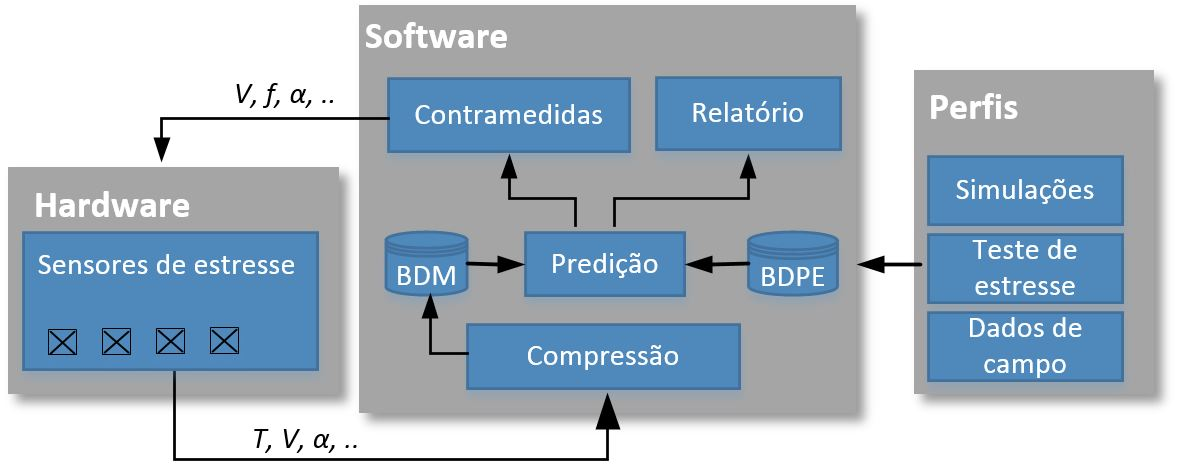
\includegraphics[width=1\textwidth]{images/sistema_proposta_metodologia}
	\caption{Abordagem proposta para análise de envelhecimento.}
	\label{figure:sistema_proposta_metodologia}
\end{figure}

Quais perfis serão definidos e como serão utilizados são decisões que podem ser tomadas pelo projetista durante o projeto. De forma geral, a unidade de \textit{Predição}, ilustrada na figura \ref{figure:sistema_proposta_metodologia}, comunica-se com duas bases de dados: uma responsável por armazenar os perfis \textit{online} medidos pelos sensores e eventualmente comprimidos pela unidade de \textit{Compressão}; e a outra por armazenar perfis pré-existentes que foram criados \textit{offline}, durante o projeto ou atualizados posteriormente, durante a operação do sistema. Essas bases são denominadas, para este trabalho, de Banco de Dados de Medições (BDM) e Banco de Dados de Perfis Envelhecidos (BDPE), respectivamente.

Através de um método de estimativa (que fica a critério do projetista), a unidade de \textit{Predição} estima qual é o tempo de vida restante do sistema e em seguida envia esta informação à unidade de \textit{Contramedidas}. Esta, por sua vez, realiza alguma ação objetivando mitigar a degradação do sistema, quando for o caso. Concomitantemente, essas informações são enviadas a uma unidade de \textit{Relatório}, onde serão armazenadas.

Caso decida por mitigar a degradação, a unidade de Contramedida deve enviar sinais de controle que permitam ao Hardware alterar os parâmetros que estão contribuindo com o envelhecimento do sistema (\textit{p. ex.} tensão de operação, grau de atividade).

A abordagem apresentada acima é generalista e flexível. Isso significa que ela independe de quais parâmetros se deseja obter através dos sensores, de quais métodos sejam utilizados para predição dos MTTFs ou de onde se originam os perfis do BDPE: se são provenientes de simulações, testes de estresse ou dados de campo.

Outra vantagem desta abordagem é a capacidade de popular o banco de dados de perfis com novas observações durante a atual operação do sistema. Um BDPE que, por exemplo, possuía dados provenientes de simulações \textit{offline} pode, à medida que o sistema envelhece, ter seu conteúdo atualizado com dados de campo, melhorando as estimativas posteriores. Ainda mais: é possível que os modelos utilizados sejam atualizados com melhorias provenientes de otimizações ou até mesmo substituídos por modelos diferentes e melhores.

Posto isso, nas seções subsequentes serão descritas as técnicas e métodos utilizados neste trabalho e utilizará a figura \ref{figure:sistema_proposta_metodologia} como referência.

\section{Sensores}
O uso de sensores para observação de grandezas como temperatura, variações de tensão, grau de atividade e corrente de fuga é bem conhecido e objetivo de inúmeras pesquisas. Diversos deles são projetados especificamente para medir desgastes provenientes dos mecanismos de HCI, BTI e TDDB \cite{Kim2010}\cite{Keane2010}\cite{Kim2008}\cite{Karl2008}, descritos na seção \ref{subsection_Conf_CI}.

Entretanto, neste trabalho é considerado o uso de sensores de estresse para obtenção dos perfis de operação, medindo parâmetros como temperatura, tensão de alimentação ou grau de atividade. Um sensor de atividade realiza o monitoramento das entradas primárias de um sistema ou de uma parte delas para auxiliar na estimativa de estresse. Como exemplo de um sensor de atividade, pode-se utilizar circuitos que observem a variação das entradas e associe a cada transistor a existência ou não de degradação \cite{Baranowski2015}. A figura \ref{figure:monitor_atividades} mostra um exemplo genérico que auxilia o entendimento desta abordagem, onde $E1, E2$ e $E3$ são sinais de entrada que podem alterar o sinal de saída $S$:
\begin{figure}[H]
	\center
	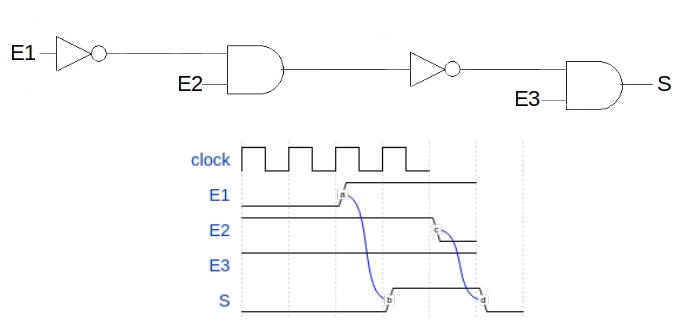
\includegraphics[width=0.7\textwidth]{images/monitor_atividades}
	\caption{Alteração das entradas refletem-se como uma atividade nas portas lógicas.}
	\label{figure:monitor_atividades}
\end{figure}

No exemplo, o sinal da entrada $E1$ é alterado após um período de tempo, mudando o sinal da saída $S$. O mesmo ocorre para a entrada $E2$. Na técnica de monitoramento do grau de atividade, essas alterações podem resultar em uma degradação das portas lógicas que estão presentes no caminho percorrido pelo sinal que vai desde $E1$ até a $S$: duas portas NOT e duas AND2.

Isso significa que, a mudança dos sinais $E1$, $E2$ e $E3$ pode alterar como os transistores de cada porta lógica se comportam (\textit{p.ex.} número de transistores pMOS ativos das portas AND2 do exemplo). Esse comportamento, por sua vez, pode estar associado a um envelhecimento maior ou menor dos transistores decorrentes da degradação por NBTI, por exemplo.

Uma vez determinada essa atividade e a degradação, elas são associadas entre si para que futuras degradações sejam estimadas. O aumento da área total do sistema, decorrente da inserção destes circuitos de monitoramento, é dependente da quantidade de circuitos do sistema a serem monitorados e da precisão desejada na estimativa da degradação \cite{Baranowski2015}.

Já para o caso de sensores de temperatura e tensão de alimentação, a frequência com que essas grandezas variam ao longo do tempo impõem restrições no que se refere ao seu armazenamento, visto que armazenar cada transição de temperatura, por exemplo, exigiria dos sensores ou da unidade de Compressão uma capacidade de armazenamento restritiva. Isto por sua vez aumentaria a área total do sistema, o que pode ser ainda mais restritivo em muitos casos.

Fica então a cargo do projetista escolher qual será a frequência de coleta dos dados ou se será usada alguma métrica que represente a grandeza desejada para um intervalo de medição (p.ex. a temperatura média em um período de tempo $\delta t$). É necessário salientar que esta abordagem incorre na redução de precisão na aferição realizada pelos sensores.

Em contrapartida, a memória necessária para armazenar estas informações é consideravelmente menor. Para este trabalho será considerado que uma métrica (como a média) foi utilizada para descrever as informações de operação do sistema, que posteriormente serão inseridas tanto o BDM quanto no BDPE.
\section{Geração de perfis}
\label{section_obtencao_dados}
No contexto exposto acima, onde um conjunto de sensores amostram condições ambientais, é preciso estabelecer quais informações se deseja representar ao armazenar estas condições. O intuito desta representação é permitir que seja estimado o MTTF, e consequentemente o RUL, de um sistema. 

Para este trabalho são utilizadas a tensão de alimentação $V$ e temperatura $T$ como condições ambientais a serem representadas no BDM e BDPE. A literatura e pesquisas exploradas na seção \ref{subsection_estado_da_arte} evidenciam uma forte relação entre $V$ e $T$ com os efeitos de degradação explanados na seção \ref{subsection_Conf_CI}.

Considerando que as condições ambientais impostas ao sistema variam com sua operação, podemos exemplificar os valores de temperatura obtidos por um sensor $S_{T,4}$ ao longo de $t$ como mostrado na figura \ref{figure:profile_sets}. Neste período o sistema está operando sob diversas faixas de temperatura $T$, denominadas de \textit{Conjunto 1, Conjunto 2, Conjunto 3, Conjunto 4 e Conjunto 5}. Os sensores serão agrupados pelo seu tipo $k$ (\textit{p.ex.} Temperatura $T$, tensão de alimentação $V$ ou atividade $\alpha$) e denotados por $s_{k,i}$, sendo $i$ o índice de um sensor específico (\textit{p.ex.} 1,\ 2,\ 3,\ \dots).

\textit{Exemplo:} Um sistema possui 6 sensores, sendo dois de temperatura e quatro de tensão de alimentação. Os dois sensores serão denotados por $s_{T,1}$ e $s_{T,2}$. Já os de tensão são denotados como $s_{V,1}$, $s_{V,2}$, $s_{V,3}$ e$s_{V,4}$.

Isso significa que, para cada sensor $s_{k,i}$ existe um vetor $S_{k,i}[\ ]$ com $N$ conjuntos para cada sensor. Um elemento $n$ do vetor $S_{k,i}[\ ]$ quantifica o tempo de permanência do sensor $s_{k,i}$ em uma determinada faixa de valor.
\begin{figure}
\center
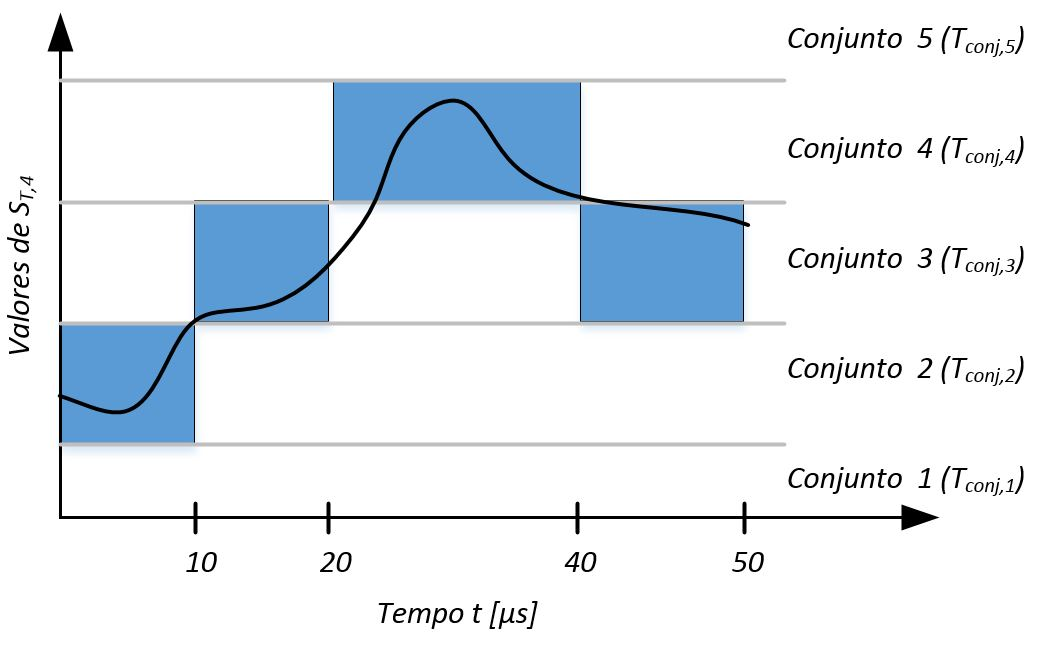
\includegraphics[width=0.8\textwidth]{images/profile_sets}
\caption{Compressão dos dados medidos e representação dos mesmos através de perfis de envelhecimento.}
\label{figure:profile_sets}
\end{figure}

No exemplo mostrado na figura \ref{figure:profile_sets}, para uma medição realizada em um período $\Delta t=10 \mu s$ e um vetor $S_{T,4}[\ ]$ inicialmente vazio, o sensor $s_{T,4}[\ ]$ permanece no conjunto 2 de $t=0 \mu s$ a $t=10 \mu s$. Consequentemente, $S_{T,4}[2]$ recebe o valor 10. Seguindo esta lógica o vetor resultante após 50$\mu s$ é $S_{T,4} = [0,10,20,20,0]$.

A criação dos conjuntos de perfis permite quantificar o estresse aplicado ao sistema e a relação entre os parâmetros dos perfis e o tempo de vida esperado dos circuitos monitorados pelos sensores. Cada perfil é inserido no BDPE conforme exposto na tabela \ref{tb:BDPE}.

Cada linha $w$ contém o percentual de tempo $p_{T(w,x)}$ e $p_{V(w,y)}$ sob os quais um ou mais circuitos monitorados estão submetidos a uma temperatura pertencente ao conjunto $T_{conj,x}$ e uma tensão de alimentação que pertence ao conjunto $V_{conj,y}$ ; sendo $x$ e $y$ os índices dos conjuntos utilizados para descrever o sistema (\textit{p. ex.} $x = 1,\ 2, \ \dots,\ X$ e $y = 1,\ 2,\ \dots,\ Y$).

Como exemplo, a primeira linha ($w=1$) informa que os circuitos monitorados experimentam durante um percentual $p_{T(1,1)}$ de seu tempo de operação $t_{oper}$ uma temperatura pertencente ao conjunto $T_{conj,1}$, um percentual $p_{V(1,1)}$ para uma tensão de alimentação pertencente ao conjunto $V_{conj,1}$ e assim por diante para as colunas subsequentes. Ao final, é esperado que após operar sob estas condições durante $t_{oper}$ seu tempo de vida seja de $MTTF_1$.

\begin{table}[H]
\centering
\caption{Base de Dados de Perfis Envelhecidos}
\begin{tabular}{@{}l|l|l|l|l|l|l@{}}
\toprule
$T_{conj,1}$ & {...} & $T_{conj,X}$ & $V_{conj,1}$ & {...} & $V_{conj,Y}$ & MTTF \\ \midrule
$p_{T(1,1)}$ & {...} & $p_{T(1,X)}$ & $p_{V(1,1)}$ & {...} & $p_{V(1,Y)}$ & $MTTF_1$ \\
$p_{T(2,1)}$ & {...} & $p_{T(2,X)}$ & $p_{V(2,1)}$ & {...} & $p_{V(2,Y)}$ & $MTTF_2$ \\
\ \ \ {...} & {...} & \ \ \ {...} & \ \ \ {...} & {...} & \ \ \ {...} & \ \ \ \ {...} \\
$p_{T(M,1)}$ & {...} & $p_{T(M,X)}$ & $p_{V(M,1)}$ & {...} & $p_{V(M,Y)}$ & $MTFF_M$ \\ \bottomrule
\end{tabular}

\label{tb:BDPE}
\end{table}
Aplicando a abordagem anterior à figura \ref{figure:profile_sets} obtemos o excerto representado na tabela \ref{tb:BDPE_reduzida}:
\begin{table}[H]
\centering
\caption{Excerto de um BDPE com dados exemplares.}
\begin{tabular}{@{}l|l|l|l|l|l|l|l|l|l|l@{}}
\toprule
$T_{conj,1}$ & $T_{conj,2}$ & $T_{conj,3}$ & $T_{conj,4}$ & $T_{conj,5}$ & $V_{conj,1}$ & $V_{conj,2}$ & $V_{conj,3}$ & $V_{conj,4}$ & $V_{conj,5}$ & MTTF \\ \midrule
$0$ & $10$ & $20$ & $20$ & $0$ & $0$ & $10$ & $20$ & $20$ & $0$  & $MTTF_1$ \\
\bottomrule
\end{tabular}

\label{tb:BDPE_reduzida}
\end{table}
Este exemplo enfatiza a vantagem de perfis granulares (\textit{i.e} que consideram variação nos perfis durante a operação) em comparação a modelos estáticos na obtenção do RUL de um sistema. Estes perfis podem ser obtidos através de simulações de envelhecimento, dados de campo ou testes acelerados de estresse. Este trabalho propõe, no capítulo 4, um fluxo de envelhecimento que simule diversos circuitos e extraia esses perfis e utiliza-se de simuladores como os descritos na seção \ref{subsection_Simuladores}.

\section{Métodos de estimativa}
\label{section_metodos_estimativa}
Utilizando ferramentas de simulação e envelhecimento de circuitos aliados a esta abordagem de perfis, é possível estimar o tempo de vida restante de um sistema conhecido. Sendo assim, é necessário determinar a relação entre uma entrada do BDM e o BDPE; e consequentemente o tempo de vida restante. Estas informações podem ser usadas nos métodos de estimativa que serão apresentados a seguir para determinar, aproximadamente, em qual estado o circuito está e o que acontecerá se ele continuar a operar nestas condições.

Um modelo linear geral \cite{McCullagh1984} pode ser utilizado, inicialmente, para estimar a relação entre o atraso de saída e as temperaturas e tensões de entrada; mais especificamente um modelo de regressão linear simples (RLS). Uma RLS ajuda a responder às seguintes perguntas sobre o dado a ser trabalhado \cite{James2013}:
\begin{enumerate}
	\item Existe uma relação entre um conjunto de temperatura $T_{conj,x}$ ou um conjunto de tensão $V_{conj,y}$ e o MTTF?
	\item A relação pode ser descrita linearmente?
\end{enumerate}
A RLS descreve uma variável de resposta $Y$ como dependente de um conjunto de variáveis explicativas $x$ (também chamado de \textit{preditor}) da seguinte forma:
\begin{equation}
\label{eq:regressao_linear_simples}
Y \approx \beta_0+\beta_1X + \epsilon
\end{equation}
sendo $\beta_0$ e $\beta_1$ duas constantes desconhecidas que representam a interceptação da reta com o eixo vertical e a inclinação da mesma, respectivamente. Para representar uma variável ou constante desconhecida e que foi estimada através do modelo, será utilizado o símbolo$\ $ $\hat{}$$\ $. Isso significa que $\hat{y}$ indica uma predição da variável de resposta $Y$ para $X = x$.

Para se estimar $\hat{\beta_0}$ e $\hat{\beta_1}$ é necessário utilizar-se de dados pré-existentes do sistema a ser analisado. Considerando que o projetista possua $n$ observações desse sistema na forma de pares representados por $(x_1,y_1),(x_2,y_2),\dots,(x_n,y_n)$, que consistem de uma medida de $X$ e uma de $Y$, o objetivo da RLS é obter os coeficientes de $\hat{\beta_0}$ e $\hat{\beta_1}$ e um modelo linear que melhor se ajuste ao dados. Ele é descrito como:
\begin{equation}
\label{eq:RLS_estimado}
\hat{y} =\hat{\beta_0}+\hat{\beta_1}x_i
\end{equation}
sendo $i$ o índice do i-ésimo preditor.

O método mais comum de se obter este modelo é através do critério de \textit{mínimos quadrados} \cite{James2013}. Como exemplo, consideremos um conjunto de dados como os mostrados na figura \ref{figure:minimos_quadrados_exemplo} e um modelo representado pela equação \ref{eq:regressao_linear_simples}. Um i-ésimo preditor X, representado por $x_i$, tem como resultado um i-ésimo dado observado $\hat{y}$ para esta equação. 

Entretanto, ao inserir na equação \ref{eq:regressao_linear_simples} um valor de preditor $X = x_i$ cuja resposta $Y$ seja conhecida, o $\hat{y}$ calculado não necessariamente será igual ao $Y$ esperado. A diferença é conhecida como \textit{resíduo} e é representada por $\epsilon$. Assim sendo, o i-ésimo resíduo entre um $Y$ esperado e um $\hat{y}$ estimado é dado por:
\begin{equation}
\label{eq:residuo}
\epsilon_i =  Y_i - \hat{y_i}
\end{equation} 
O critério de \textit{mínimos quadrados} estima $\hat{\beta_0}$ e $\hat{\beta_1}$ de forma a minimizar a \textit{soma dos quadrados dos resíduos} (SQR) que é equivalente a:
\begin{equation}
\label{eq:SQR}
SQR = (y_1-\hat{\beta_0} - \hat{\beta_1}x_1)^2 + (y_2-\hat{\beta_0} - \hat{\beta_1}x_2)^2 + \dots + (y_n-\hat{\beta_0} - \hat{\beta_1}x_n)^2
\end{equation} 
Rearranjando as equações \ref{eq:RLS_estimado} e \ref{eq:SQR}:
\begin{equation}
\label{eq:RLS_coeficientes}
\hat{\beta_1} = \frac{\sum_{i=1}^{n}(x_i-\bar{x})(y_i-\bar{y})}{\sum_{i=1}^{n}(x_i-\bar{x})^2},
\hat{\beta_0} = \bar{y} -\hat{\beta_1}\bar{x} 
\end{equation}
onde $\bar{y}$ e $\bar{x}$ são as médias amostrais de $y$ e $x$, respectivamente.
\begin{figure}
\center
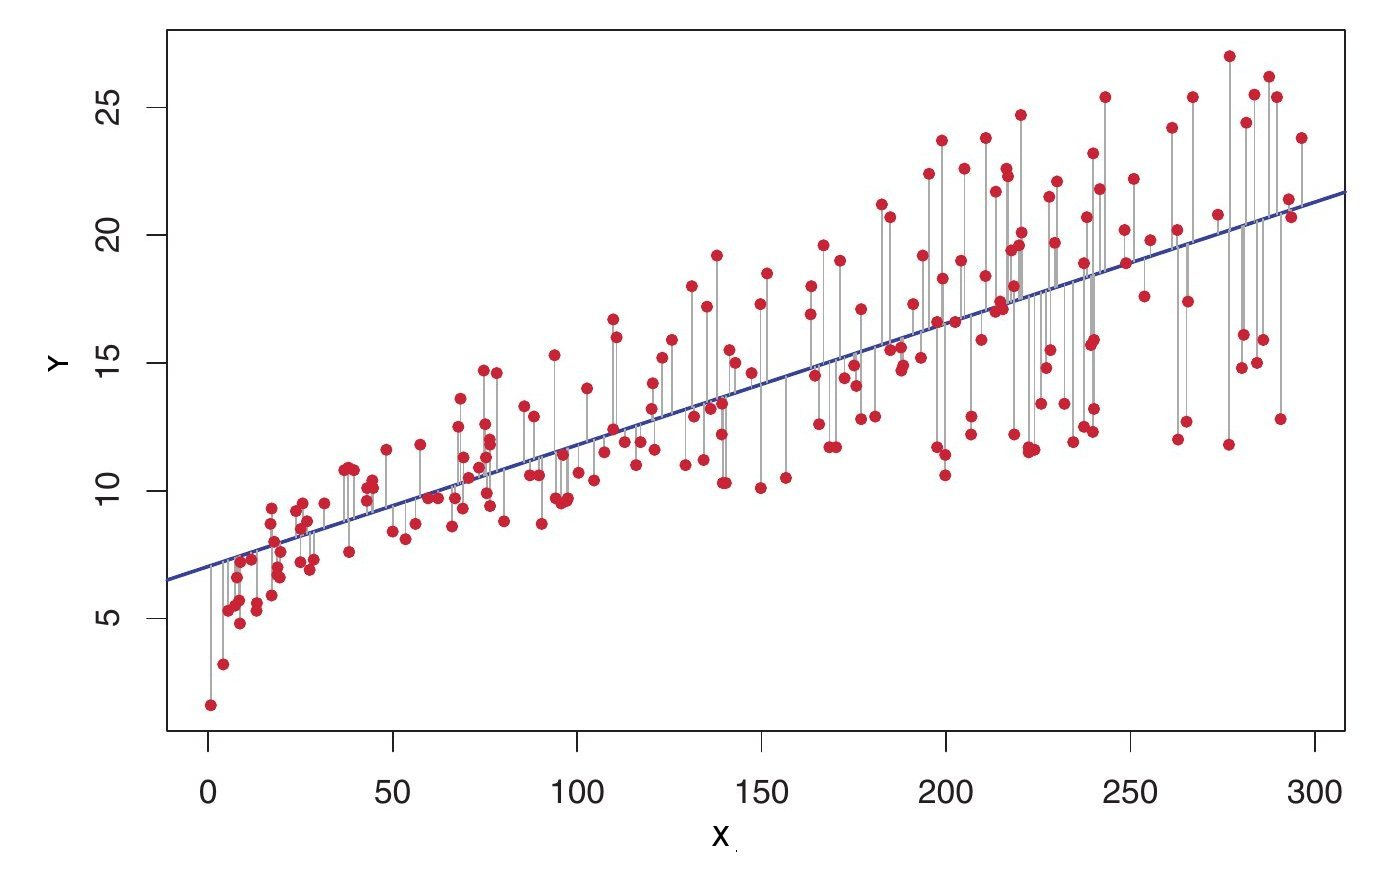
\includegraphics[width=0.8\textwidth]{images/minimos_quadrados_exemplo}
\caption{Modelo linear ajustado a um conjunto de dados de exemplo, representado pela reta azul. Os pontos vermelhos representam os dados coletados e seus respectivos resíduos \cite{James2013}.} 
\label{figure:minimos_quadrados_exemplo}
\end{figure}
Um modelo de RSE descreve de forma simples a relação entre uma grandeza, que funciona como uma variável explicativa, e outra que se deseja estimar, a variável observada.
Entretanto, para o problema que este trabalho tenta solucionar, não é suficiente relacionar somente um preditor a uma observação. Considerando um BDPE maior, representada pela tabela \ref{tb:regressao_simples_exemplo}, não é possível utilizar somente uma variável explicativa pois o MTTF será função de quatro preditores: $T_{conj,1}=30, T_{conj,2}=50, V_{conj,1}=1.0$ e $V_{conj,2}=1.1$.
\begin{table}[H]
	\centering
	\caption{Tabela de exemplo para regressão linear simples.}
	\begin{tabular}{@{}l|l|l|l|l@{}}
		\toprule
		30 & 50 & 1.0 & 1.1 & MTTF \\ \midrule
		13 & 1 & 12 & 2 & 1.2 \\
		7 & 8 & 3 & 12 & 2.7 \\
		1 & 1 & 2 & 2 & 5.3 \\
		5 & 5 & 4 & 7 & 3.5 \\		
		7 & 8 & 4 & 5 & 2.0 \\ \bottomrule
	\end{tabular}
	\label{tb:regressao_simples_exemplo}
\end{table}
Para o exemplo da tabela \ref{tb:regressao_simples_exemplo}, uma RLS não é capaz de responder os seguintes questionamentos:
\begin{enumerate}
	\item Quão forte é a relação entre conjuntos de $T_{conj,x}$, $V_{conj,y}$ e o MTTF?
	\item Qual dos conjuntos mais contribui para a redução do MTTF? 
\end{enumerate}
Considerando o exemplo da figura \ref{figure:profile_sets} e a subsequente tabela \ref{tb:BDPE_reduzida}, existem dez variáveis explicativas para uma saída desejada, \textit{p. ex.} MTTF. Realizar uma regressão para cada um dos preditores não é satisfatório. Uma melhor abordagem é expandir a RLS para uma Regressão Linear Múltipla (RLM), dando a cada preditor seu próprio coeficiente de inclinação $\beta$. Seu modelo é expresso então por:
\begin{equation}
\label{eq:regressao_linear_multipla}
Y \approx \beta_0+\beta_1X_1 +\dots +\beta_pX_p +\epsilon
\end{equation}
Assim como foi estimado para uma RLS, os coeficientes serão calculados usando o critério de \textit{mínimos quadrados}. Para os valores disponíveis na tabela \ref{tb:regressao_simples_exemplo}, os coeficientes são:
\begin{table}[H]
	\centering
	\caption{Coeficientes do modelo de RLM para o exemplo da tabela \ref{tb:regressao_simples_exemplo}.}
	\begin{tabular}{@{}l|l|l|l|l|l@{}}
		\toprule
		& Interceptação & $T_{conj,1}$ & $T_{conj,2}$ & $V_{conj,1}$ & $V_{conj,2}$ \\ \midrule
		Coeficiente & \ \ \ \ \ \ 5.765 & -0.295 & -0.242 & -0.056 & 0.092 \\ \bottomrule
	\end{tabular}
	
	\label{tb:regressao_multipla_coeficientes}
\end{table}
Entretanto uma regressão linear múltipla exige uma independência entre essas variáveis explicativas \cite{Chatterjee}, premissa que não podemos garantir dado que os percentuais $p_{T(w,x)}$ e $p_{V(w,y)}$ podem estar correlacionadas. Em adição, a degradação causada pelos conjuntos $T_{conj,x}$ e $V_{conj,x}$ serão dependentes da degradação subsequente dos conjuntos $T_{conj,x-1}$ e $V_{conj,x-1}$.

Ao invés disso, três métodos são propostos: Regressão de mínimos quadrados parciais (Partial Least Square Regression, PLS-R), Distância Euclidiana (DE) e Correlação (COR).
\subsection{Regressão de Mínimos Quadrados Parciais}
\label{subsection_estimativas_PLSR}
A Regressão de Mínimos Quadrados Parciais (PLS-R) é uma técnica que pertence à categoria dos modelos lineares generalizados e que reúne um grupo de algoritmos. Ao contrário da RLM, é menos exigente quanto a existência de correlação entre as variáveis. A PLS-R é classificada como uma abordagem que transforma os preditores e os ajusta a um modelo de mínimos quadrados utilizando-se das variáveis que foram transformadas.

Considere uma combinação linear dos preditores originais $p$ e representada por $Z_1,Z_2,\dots,Z_M$ para $M < p$, onde:
\begin{equation}
Z_m = \sum_{j-1}^{p}\alpha_{jm}X_j
\label{eq:combinacoes_lineares}
\end{equation}
sendo $\alpha_{1m},\alpha_{2m},\dots,\alpha_{pm}$ constantes e $m=1,\dots,M$.

Um modelo de regressão linear pode então ser ajustado por mínimos quadrados e equacionado como:
\begin{eqnarray}
y_i=\theta_0+\sum_{m=1}^{M}\theta_mz_{im}+\epsilon_i, i=1,\dots,n
\label{eq:RLM_PLS}
\end{eqnarray}
Neste caso, os coeficientes de regressão são dados pela constante $\theta$. É possível então definirmos valores de $\alpha$ tais que o modelo para as variáveis transformadas se mostre melhor do que o modelo original.

Por reduzido entende-se que, ao invés de estimarmos $p+1$ coeficientes $\beta_0,\beta_1,\dots,\beta_p$, são estimados $M+1$ coeficientes $\theta_0,\theta_1,\dots,\theta_M$. Dado que $M<p$, como enunciando anteriormente, a dimensão do modelo foi reduzida.

Esta abordagem é compartilhada entre os métodos de compressão. Sumarizadamente, eles possuem duas etapas:
\begin{enumerate}
	\item Obtenção dos preditores transformados $Z_1,Z_2,\dots,Z_M$.
	\item Ajuste do modelo utilizando $M$ preditores.
\end{enumerate}
Entretanto, quais e como os preditores $Z_1,Z_2,\dots,Z_M$ são obtidos varia entre métodos. A proposto em comum é de que, geralmente, uma pequena quantidade deles é suficiente para explicar a variabilidade dos dados originais e sua relação com a resposta. É assumido que a direção para as quais as entradas $X_1,X_2,\dots,X_p$ mostram uma maior variação são as mais associadas à saída Y.

Observando o exemplo da figura \ref{figure:principal_component}, é perceptível que a linha verde segue a direção para a qual as observações mais variam. Esta linha é denominada de \textit{primeiro componente principal}, representado por $Z_1$ e expresso na equação \ref{eq:combinacoes_lineares}.

\begin{figure}[H]
	\center
	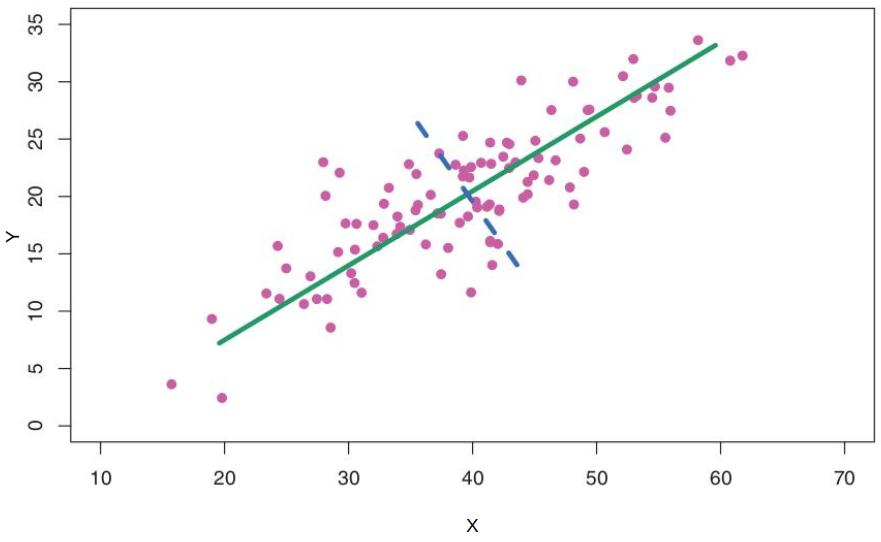
\includegraphics[width=0.8\textwidth]{images/principal_component}
	\caption{Representação de componentes principais. A linha verde representa o primeiro componente e a linha azul o segundo. \cite{James2013}.} 
	\label{figure:principal_component}
\end{figure}

Isso significa que, se os dados observados Y forem projetados nessa reta verde, as projeções apresentarão como resultado a maior variância possível se comparadas com uma projeção em qualquer outra linha que siga a variação dos dados. Em outras palavras, é o vetor que mais próximo está das observações.

Entretanto podemos obter mais componentes que ajudem a descrever os dados. Na figura \ref{figure:principal_component} um \textit{segundo componente principal} $Z_2$ é representado pela linha azul tracejada. Ele é uma combinação linear das variáveis que não estão correlacionadas à $Z_1$ e que, dada esta condição de não-correlação, apresente a maior variância possível.

Como os dados de exemplo da figura \ref{figure:principal_component} são bidimensionais, podemos obter no máximo dois componentes principais. Caso contrário, mais podem ser obtidos e sempre seguindo a premissa de que devem maximizar a variância mas sem estar correlacionados aos componentes anteriores, ou seja, são ortogonais aos mesmos.

Na técnica de \textit{Mínimos Quadrados Parciais} (Partial Least Squares, PLS), o primeiro componente $Z_1$ é obtido através do ajuste de cada $\alpha_{j1}$ da equação \ref{eq:combinacoes_lineares} para que sejam iguais aos coeficientes da regressão linear simples de Y sobre $X_j$ \cite{James2013}. Em seguida, o segundo componente $Z_2$ é computado de forma similar ao $Z_1$, porém utiliza os resíduos obtidos da regressão de $Z_1$.

Os dados residuais são interpretados como sendo a informação remanescente que não foi explicada pelo primeiro componente principal. Os resíduos são então projetados ortogonalmente e o $Z_2$ obtido através de uma regressão linear destes dados.

Essa técnica implica que os dados do BDPE e BDM podem ser reduzidos para uma representação de menor dimensão \cite{Maitra2008}. O PLS tenta maximizar a variância dos estimadores e auxilia a identificar quantos deles são necessários para explicar os dados do BDM e BDPE. É possível então descrever o MTTF de um sistema como uma RLM cujos coeficientes são iguais aos componentes obtidos.

Assim sendo, o MTTF será uma função dessa regressão e pode ser expressada da seguinte forma:
\begin{equation}
MTTF = \hat{y}= \hat{\beta_0}x_0+\hat{\beta_1}x_1+\dots+\hat{\beta_n}x_n
\label{eq:MTTF_estimadores}
\end{equation}
onde $\beta_i$ são o ponto de interceptação da reta e coeficientes da RLM e que ajustam a contribuição dos estimadores $x_i$. A quantidade $i$ de estimadores pode ser determinada pelo projetista, que deve procurar a quantidade de estimadores que melhor explique seus dados. 

\subsection{Distância Euclidiana}
\label{subsection_estimativas_euclidiana}
A Distância Euclideana é definida como a representação da distância entre dois pontos representados no espaço euclideano \cite{Deza2009}. Esta métrica é particularmente útil pois permite uma representação trivial da distância entre dois elementos que se deseja analisar.

Na PLS-R é feita uma estimativa a partir de dados pré-existentes e um modelo linear é obtido. Entretanto, na DE é possível se estimar qual dos perfis $p_{T(w,x)}$ e $p_{V(w,y)}$ pré-existentes no BDPE mais se aproxima do perfil medido pelos sensores. Essa proximidade é dada pela distância euclidiana.

A distância $d(a,b)$ entre duas séries de pontos $a=(a_1,a_2,\dots,a_N)$ e $b=(b_1,b_2,\dots,b_N)$ com N valores cada pode ser representada pela expressão seguinte:

\begin{equation}
d(a,b)=\sqrt{\sum_{i=1}^{N}(a_i-b_i)^2}
\label{eq:dist_euclideana}
\end{equation}

Para a estimativa do MTTF, é necessário calcular a distância entre cada entrada do BDPE e o perfil obtido pelos sensores. Usando como exemplo o BDPE representado na tabela \ref{tb:regressao_simples_exemplo}, que possui 4 dimensões para suas variáveis explicativas, as distâncias euclideanas para um perfil dado, por exemplo, por $S_{T,4} = [3,8]$ e $S_{V,4} = [9,6]$ são dadas como:

\begin{align}
d(a_1,b_1) = \sqrt{(13-3)^2+(1-8)^2+(12-9)^2+(2-6)^2} = 13.19 \\
d(a_2,b_2) = \sqrt{(7-3)^2+(8-8)^2+(3-9)^2+(12-6)^2} = 9.38 \\
d(a_3,b_3) = \sqrt{(1-3)^2+(1-8)^2+(2-9)^2+(2-6)^2} = 10.86 \\
d(a_4,b_4) = \sqrt{(5-3)^2+(5-8)^2+(4-9)^2+(7-6)^2} = 6.24 \\
d(a_5,b_5) = \sqrt{(7-3)^2+(8-8)^2+(4-9)^2+(5-6)^2} = 6.48
\end{align}

Logo, o perfil de menor distância euclidiana dentre os armazenados no BDPE é o quarto. Consultando a tabela \ref{tb:regressao_simples_exemplo}, o MTTF pertencente à entrada do BDPE que possui a menor distância euclideana é utilizado então para mensurar o tempo de vida restante do sistema. No exemplo fictício desta tabela é estimado que o $MTTF=3.5$.
\subsection{Correlação de Pearson}
\label{subsection_estimativas_correlacao}
Um terceiro método proposto foi a utilização da Correlação, que essencialmente mostra a dependência e associação entre duas ou mais variáveis \cite{Rodgers1988}. Para identificar uma possível relação entre os dados a serem analisados é definido um \textit{coeficiente de correlação}. É de suma importância salientar que esta métrica não necessariamente implica em causalidade.

Existem diferentes métodos para análise de correlação. Entre eles existe a \textit{Correlação r de Pearson} (CP), também conhecida como \textit{correlação paramétrica}. Ela calcula a dependência linear entre duas variáveis X e Y, um coeficiente cuja representação simbólica é $r$, e que varia entre $+1$ e $-1$. Um valor $r$ que se aproxima cada vez mais de $\pm1$ é interpretado como um grau de associação ``perfeita'' entre duas variáveis. Caso $r$ se aproxime de $0$, é dito que não há correlação ou ela é fraca.

A sinalização $\pm$ indica apenas a direção da correlação, sendo positiva para ``$+$'' e negativa para ``$-$''. Isso significa que em uma correlação positiva, quando uma das variáveis cresce ou decresce em valor, a outra variável acompanha o mesmo sentido de acréscimo ou decréscimo. O contrário pode ser dito da correlação negativa.
A correlação entre dois vetores $x$ e $y$ é quantificada pelo seu coeficiente $r_{x,y}$ e pode ser descrito por:

\begin{align}
r_{x,y}= \frac{\sum_{i=1}^{n}(x-\bar{x})(y-\bar{y})}{\sqrt{\sum_{i=1}^{n}(x-\bar{x})^2 \sum_{i=1}^{n}(y-\bar{y})^2}} \\
r_{x,y}=\frac{cov(x,y)}{\sigma_x,\sigma_y}
\label{eq:correlacao}
\end{align}

onde $cov$ é a covariância; $\bar{x}$ e $\bar{y}$ são as médias de $x$ e $y$; $n$ é o tamanho desses vetores e $\sigma$ é o desvio-padrão da série \cite{Chatterjee}.

Considerando a tabela \ref{tb:regressao_simples_exemplo}, um perfil de interesse dado por $S_{T,4} = [3,8]$ e $S_{V,4} = [9,6]$, os coeficientes de correlação $r$ entre cada perfil da tabela e o perfil de interesse é:
\begin{equation}
r = [-0.2963478, -0.3748790,  0.4364358, -0.3504383, -0.3450328]
\end{equation}
Estamos interessados no resultado com maior correlação dentre eles, no caso $r_4=0.4364358$. Esse coeficiente corresponde à correlação do 3º perfil da nossa tabela de exemplo, cujos valores das variáveis estimativas são $S_{T,4} = [3,8]$, $S_{V,4} = [9,6]$ e seu $MTTF=5.3$.

Em suma, é realizado o cálculo da correlação entre o perfil medido e a as entradas do BDPE, encontrando-se aí a entrada de menor correlação e seu respectivo MTTF.

% Aging flow
% ----------------------------------------------------------
\chapter{Fluxo de envelhecimento de circuitos integrados}
\epigraph{\textit{Open your mind to what I shall disclose, and hold it fast within you; he who hears, but does not hold what he has heard, learns nothing.}}{-Dante Alighieri}
Um dos pontos mais importantes para a simulação e obtenção de dados que deem apoio às futuras pesquisas e projetos é a decisão de quais soluções técnicas, das disponíveis, será utilizada para obter resultados coerentes com experimentos reais. Este é um ponto crucial deste trabalho pois os dados obtidos e o comportamento observado devem dar apoio à tomada de decisões por parte de sistemas que atuam na recuperação de falhas.

Para garantir esta fidelidade, foi escolhida a ferramenta Relxpert$^{\textcopyright}$. Este simulador é desenvolvido especialmente para cálculo de envelhecimento de circuitos integrados e considera efeitos como HCI, TDDB e NBTI/PBTI. Dada à experiência e proximidade da Cadence com o mercado de semicondutores, temos disponível uma ferramenta confiável para simulação e extração de resultados.

Outro fator importante é o uso de parâmetros de envelhecimento coerentes com os dispositivos reais. Ao evitar a modelagem destes parâmetros (e da criação de modelos para os efeitos de HCI, TDDB e BTI) é possível integrar a solução aqui apresentada a qualquer modelo. Como resultado, é proposta uma solução independente das ferramentas escolhidas, da tecnologia empregada e da metodologia utilizada no cálculo dos parâmetros.

Para nossa conveniência, utilizamos parâmetros disponibilizados pela própria ferramenta e que se assemelham às tecnologias de 90nm empregada pelas \textit{foundries} de dispositivos semicondutores.

\section{Estratégia do fluxo}
\label{section_estrategia_fluxo}
O fluxo de envelhecimento para extração é composto de seis etapas principais sumarizadas abaixo e representadas na figura \ref{figure:fluxo_geral}:
\begin{enumerate}
	\item Criação de uma tabela com condições ambientais pré-estabelecidas;
	\item Identificação de um caminho crítico para análise e criação de uma \textit{netlist} primitiva;
	\item Envelhecimento da \textit{netlsit} primitiva e criação de uma envelhecida;
	\item Simulação da netlist envelhecida;
	\item Extração dos atrasos relativos e do MTTF;
	\item Criar e popular um BDPE.
\end{enumerate}
\begin{figure}[H]
\center
{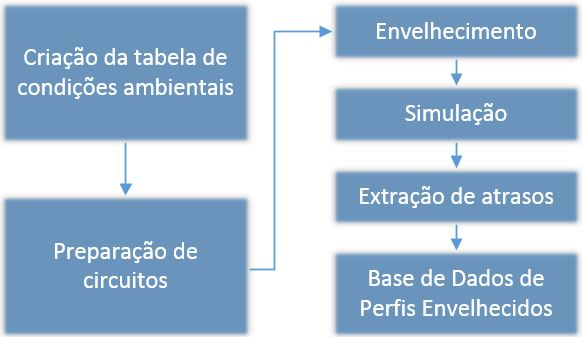
\includegraphics[width=0.7\textwidth]{images/fluxo_geral}}
\caption{Fluxo geral utilizado no envelhecimento de circuitos integrados.}
\label{figure:fluxo_geral}
\end{figure}
É importante salientar que esta é apenas uma das forma de se popular a base de dados de perfis envelhecidos, conforme mencionado na seção \ref{section_visao_geral}, e pode ser utilizada em conjunto com as demais técnicas mencionadas na seção. Para este trabalho, esta tabela de condições ambientais servirá um duplo propósito: representar o BDM e o BDPE. No capítulo 5 é detalhado como esta tabela é utilizada na criação dos modelos de predição de MTTF.

A simulação \textit{offline} do sistema a ser observado (ou de parte dele) exige algumas \textit{entradas} a serem utilizadas no fluxo de envelhecimento:
\begin{enumerate}
\item Um conjunto de netlists a serem envelhecidas. Neste trabalho são utilizadas netlists cuja sintaxe é \textit{Spectre};
\item Os arquivos de modelos para os dispositivos do tipo nMOS e pMOS. Estes arquivos contém não somente os parâmetros de operação como também os de envelhecimento;
\item Uma tabela de condições ambientais a serem aplicadas ao sistema. No trabalho foram utilizados os modelos BSIM4 \cite{Karl2008}.
\end{enumerate}
Como \textit{saída} são obtidos:
\begin{enumerate}
\item Uma netlist com cada parâmetro de envelhecimento que será usado na simulação envelhecida;
\item Dados de simulação da netlist envelhecida e atrasos relativos à uma saída pré-determinada.
\end{enumerate}

Durante este processo de envelhecimento, etapas intermediárias são necessárias, conforme mostrado na figura \ref{figure:fluxo_ferramenta}:
\begin{enumerate}
	\item Cálculos de envelhecimento: etapa onde são obtidas as variações de parâmetros dos dispositivos empregados e como degradam com o tempo. Além disso, uma netlist ``pré-processada'' é criada. Isso significa que ela já foi modificada com as condições ambientais necessárias para a simulação envelhecida mas sem as informações de degradação dos dispositivos que a compõe. Estas mudanças são retiradas dos arquivos de modelo e informam como a tensão de limiar $V_{TH}$ de um transistor nMOS, por exemplo, aumenta com o decorrer do envelhecimento. 
	\item Degradação de transistores: a ferramenta envelhece os dispositivos e anexa estas informações em um ou mais arquivos de modelos. Esses arquivos são atualizações baseadas nas informações originais e possuem novos valores para alguns parâmetros (\textit{p.ex.} tensão de limiar). Estes dispositivos são atualizados de forma a refletir quais serão os valores destes parâmetros após um certo período de tempo. Exemplo: considere que, em seu estado original, um dispositivo nMOS possui um $V_{TH}=1.1V$. Após simular dois anos de envelhecimento para sistema, seus transistores nMOS passam a precisar de $V_{TH}=1.23V$. Este incremento de 0.13V é consequência da degradação do sistema ao longo desses 2 anos. 
\end{enumerate}

\begin{figure}[H]
\center
{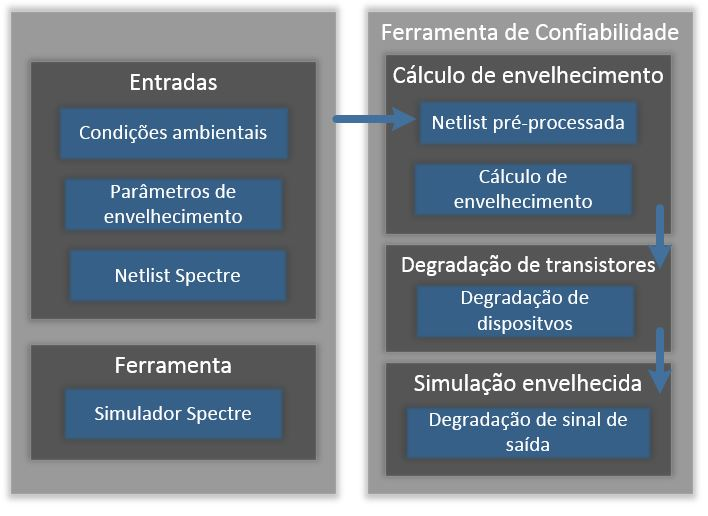
\includegraphics[width=0.7\textwidth]{images/fluxo_ferramenta}}
\caption{Entradas e saídas da ferramenta de envelhecimento.}
\label{figure:fluxo_ferramenta}
\end{figure}
Estas etapas de cálculo são realizadas pela ferramenta de envelhecimento e são ``transparentes''. Isso significa que não há, normalmente, uma intervenção por parte do projetista sobre estes cálculos, que seguem os modelos da própria ferramenta e os parâmetros de tecnologia fornecidos pela fabricante. É possível, entretanto, analisar quais mudanças e resultados são inseridos nos diversos arquivos utilizados pelos simuladores.
\section{Implementação do fluxo e integração com as ferramentas de envelhecimento}
\label{section_implementacao}
As seções seguintes irão descrever as etapas necessárias para a criação e integração do fluxo com as ferramentas e a metodologia apresentada no capítulo 3. São dados mais detalhes da preparação das \textit{netlists}, dos perfis de envelhecimento e da análise dos caminhos críticos.
\subsection{Preparação de células lógicas e netlists}
\label{subsection_celulas}
Para representar o comportamento de um sistema são, por vezes, utilizadas \textit{netlists}, que são arquivos cuja função é descrever como um sistema ou diversos componentes eletrônicos se interconectam. A netlist pode conter fios, pinos, parâmetros elétricos, regimes de operação (\textit{p. ex. temperatura, tempo de envelhecimento}), diretivas de simulação, referência a modelos de transistores, fontes de tensão e corrente, lógica booleana, entre outras informações.

Entretanto é preciso diferenciar as netlists geralmente disponíveis em um projeto de circuitos digitais:
\begin{enumerate}
	\item descrição comportamental: utilizando-se de uma linguagens de descrição de hardware (HDL), especificam o comportamento de um sistema. A descrição é de \textit{alto nível}, não contendo detalhes de quais portas lógicas são utilizadas para implementar a lógica desejada;
	\item descrição estrutural: ainda utilizando HDL, descreve uma lógica através da interconexão entre portas lógicas;
	\item descrição esquemática: detalha a interconexão entre os transistores além de possuir informações sobre fontes de alimentação, fios, elementos capacitivos, modelos de transistores, temperatura de operação e qualquer outra informação necessária para a simulação dos circuitos descritos.
\end{enumerate}

Para o fluxo aqui apresentado é proposto a utilização de uma netlist esquemática pois, por possuir a descrição dos transistores, pode conter também os parâmetros de degradação dos mesmos. Entretanto, caso o projetista não possua o esquemático, é possível obtê-lo através de uma descrição comportamental ou estrutural. Para isso, um processo de síntese ou tradução é realizado com o auxílio de softwares de \textit{projeto de circuitos integrados} (\textit{i.e.} Electronic Aided Design, EAD). Por síntese entende-se o processo de interpretação da descrição de alto nível de um circuito ou conjunto de circuitos e tradução para uma representação de portas lógicas. Define-se por tradução como sendo o processo de representar uma netlist estrutural em uma esquemática.

Caso o ponto de partida seja uma descrição comportamental, uma netlist estruturada é obtida por síntese e em seguida uma netlist esquemática. Em uma descrição comportamental não existe informação de quais portas lógicas são utilizadas, apenas as funcionalidades do sistema. Como as portas são desconhecidas, não é possível determinar quais transistores serão utilizados e, consequentemente, como os efeitos de degradação afetam os mesmos. Posteriormente, a descrição estrutural será traduzida para uma esquemática contendo todos os transistores necessários para implementar as funcionalidades projetadas.
 
Essa tradução necessita de uma biblioteca de portas lógicas que, por sua vez, possui informações detalhadas de como elas são implementadas para uma determinada tecnologia de um fabricante específico. Esta biblioteca é fornecida pelas \textit{foundries} e sua descrição detalhada foge do escopo deste trabalho. O fluxo proposto assume que a implementação destas portas já está disponível e que é possível sintetizá-las, separadamente ou em conjunto, para que uma netlist seja gerada.

Para a utilização de um sistema no fluxo que está sendo proposto é mister identificar como ele está descrito (descrição comportamental, estrutural ou esquemática) e obter gradativamente, quando necessário, a netlist esquemática.

\subsection{Preparação dos perfis de envelhecimento}
\label{subsection_perfis}
O circuitos integrados atuais trabalham sobre condições de operação que oscilam constantemente. Podemos abordar estas variações de inúmeras maneiras. Entretanto, esse trabalho considera duas abordagens complementares que propõem interpretar as variações de duas maneiras:
\begin{enumerate}
	\item Para um intervalo de tempo $t$, as variações são sumarizadas como as médias das tensões aplicadas e temperaturas medidas no dispositivo ao longo desse tempo. Isso significa que, se um sensor $S_{V,1}$ registrou uma média de $1.1V$ e um outro $S_{T,1}$ registrou uma média de $45^{o}C$, aquele intervalo será caracterizado por $V_{conj,1}=1.1$ e $T_{conj,1}=45$;
	\item Um perfil de envelhecimento representa um conjunto de intervalos (ou faixas) sob os quais o sistema esteve submetido ao longo de sua operação, conforme mostrado na figura \ref{figure:profile_sets}. Ao se variar a quantidade de tempo sob qual o circuito permanece em cada elemento deste conjunto, obtemos uma tabela que possui um sumário das condições ambientais impostas ao sistema.
\end{enumerate}
Assim sendo, existe uma tabela que associa variações de temperatura e tensão a um ciclo de vida de um sistema. Cada variação dos parâmetros de tensão de alimentação $V_{DD}$ das portas lógicas e da temperatura $T$, é associada a um tempo de operação, conforme exemplificado na tabela \ref{tb:BDPE_reduzida}. A definição dos valores $p_{T(w,x)}$ e $p_{V(w,y)}$ e da quantidade de conjuntos $T_{conj,X}$ e $V_{conj,Y}$, descritos na tabela \ref{tb:BDPE}, influencia diretamente na precisão das simulações a serem realizadas.

Para exemplificar, consideremos um sistema analisado durante 1 ano cujos perfis de operação são sumarizados pela tabela \ref{tb:regressao_multipla_exemplo2} abaixo:
\begin{table}[H]
	\centering
	\caption{Tabela de exemplo utilizada para o cálculo das variações de perfis.}
	\begin{tabular}{@{}l|l|l|l|l@{}}
		\toprule
		30 & 50 & 1.0 & 1.1 & MTTF \\ \midrule
		13 & 1 & 12 & 2 & 1.2 \\
		7 & 7 & 9 & 5 & 2.0 \\ \bottomrule
	\end{tabular}
	\label{tb:regressao_multipla_exemplo2}
\end{table}

Para o primeiro registro, o sistema fica submetido a $T_{conj,1}=30$ e $T_{conj,2}=50$ durante 1 ano. Entretanto, $T_{conj,1}=30$ influencia o sistema por mais tempo, pois possui um valor de $p_{T(w,x)}$ maior. Somando-se os valores de $p_{T(w,x)}$ para ambos os conjuntos de temperatura, o sistema é descrito como tendo sido submetido a uma temperatura média de $30^{o}C$ treze vezes ao longo de 1 ano e somente uma vez à temperatura média de $50^{o}C$, totalizando 14 intervalos de tempo $\Delta t$.

Desta forma, para um tempo de simulação $t_{sim}$ e $N$ intervalos, cada $\Delta t$ corresponde a um período de tempo dado por:

\begin{equation}
\Delta t = \frac{t_{sim}}{N}
\end{equation}

No exemplo acima $\Delta t\approx 0.07$ anos. Caso o sistema seja representado pelo BDPE da tabela \ref{tb:BDPE_reduzida}, por exemplo, seu perfil possui então $N=50$ intervalos distribuídos entre 5 conjuntos de médias de temperatura e tensão de alimentação, tornando o perfil mais granular. Como é necessário representar o mesmo sistema em diferentes intervalos de tempo, e cada intervalo pode ter suas próprias condições ambientais, o fluxo necessita de $N$ representações esquemáticas.

Essa granularidade altera a quantidade de etapas necessárias para o fluxo, conforme representado na figura \ref{figure:fluxo_detalhado}:

\begin{figure}[H]
	\center
	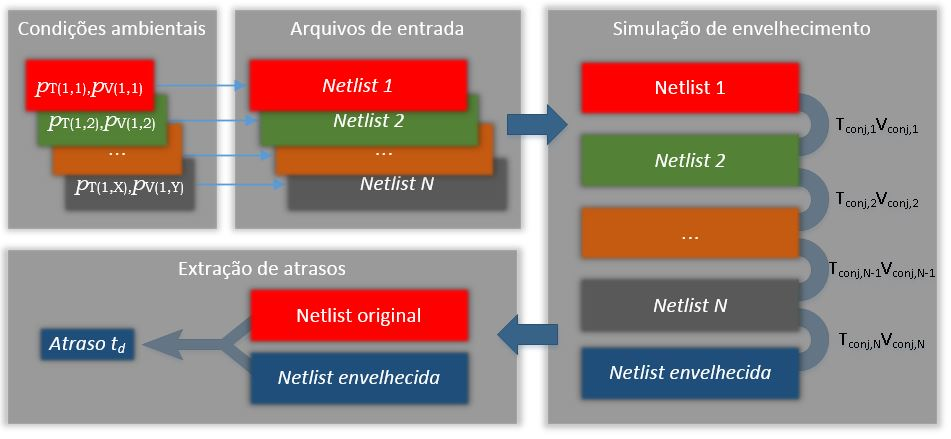
\includegraphics[width=1\textwidth]{images/fluxo_detalhado}
	\caption{Detalhamento do fluxo de criação, modificação e extração de resultados.}
	\label{figure:fluxo_detalhado}
\end{figure}

Cada uma das $N$ condições ambientais, representado no bloco \textit{condições ambientais} da figura \ref{figure:fluxo_detalhado}, será utilizada na criação de $N$ netlists, cada uma com seus respectivos $p_{T(w,x)}$ e $p_{V(w,y)}$. A degradação é realizada em $N$ etapas ao longo de um tempo $t_{sim}$, onde cada netlist é degrada durante um intervalo $\Delta t$.

Para o exemplo da tabela \ref{tb:regressao_multipla_exemplo2}, se o sistema estiver sendo observado durante 1 ano, a \textit{netlist 1} estará submetida à $T_{conj,1}=30$ e $V_{conj,1}=1.0$ durante $0.07$ anos na primeira etapa. A \textit{netlist 2} é criada e alterada com as novas condições (que para este exemplo são as mesmas), que também prevalecerão durante $0.07$ anos. Esse processo se repete até que todas as $N$ netlists sejam criadas.

Dado o exposto anteriormente, o projetista precisa preencher o BDPE com dados que provem de simulações, testes de estresse ou extraídas de campo. Neste trabalho os BDPEs foram preenchidas com dados de simulação exclusivamente e os valores de $p_{T(w,x)}$ e $p_{V(w,y)}$ foram gerados aleatoriamente, por conveniência. Essa escolha pode obedecer uma distribuição normal, caso seja adequado. A metodologia aqui proposta é indiferente quanto à essa escolha.

\section{Extração de caminhos críticos}
\label{section_extracao_caminhos}
Todas as descrições esquemáticas geradas na seção \ref{subsection_perfis} são simuladas uma após a outra. Entretanto, representar cada transistor de um sistema pode ser impraticável. Isso se deve ao fato de que os processadores mais recentes possuem bilhões de transistores \cite{Alcorn2016}, tornando a etapa de degradação de todos eles inviável e computacionalmente custosa. Além disso, para uma simulação adequada, é necessária a ativação de todas as entradas do sistema, o que também pode ser impeditivo.

Para mitigar este problema, é possível se realizar a análise temporal estática do \textit{pior caminho} de um sistema, sendo considerada uma técnica conservativa e bem estabelecida, apesar de não ser a mais moderna \cite{Orshansky2002}. O \textit{pior caminho} representa o trecho condutivo mais crítico ao sistema, onde qualquer violação de temporização torna a operação do sistema não confiável.

Dessa forma, realizar a degradação do caminho crítico é uma abordagem vantajosa e mais realística pois obtém uma quantidade reduzida de transistores e entradas a serem ativadas. Um problema desta abordagem é que não há garantia de que, após a degradação, este caminho continue sendo o mais crítico. Para mitigar este problema, mais de um caminho pode ser utilizado e posteriormente selecionado como pior aquele cuja atraso seja o maior.

A extração dos caminhos críticos é realizada pelas próprias ferramentas de EDA, que são capazes de reportar quantos caminhos forem desejados pelo projetista, gerar uma descrição esquemática e criar fontes de alimentação que ativem os piores caminhos.
\section{Simulação e degradação}
\label{section_simulacao}
Uma vez criadas as netlists e o BDPE, a degradação é realizada de fato. Foram realizadas as etapas dos blocos de ``condições ambientais'' e ``Arquivos de entrada'' representados na figura \ref{figure:fluxo_detalhado}. Para a simulação, um conjunto de rotinas irá, obedecendo o BDPE, usar a ``Netlist 1'' como argumento para o Relxpert$\textcopyright$ (software usado para a degradação).

Como saída são obtidas uma netlist degradada com seus parâmetros de operação atualizados. Isso significa que grandezas tais como tensão de limiar $V_{TH}$ e corrente de fuga $I_l$ são alteradas para refletir o desgaste sofrido pela primeira netlist. Em adição, parâmetros de degradação existentes nos modelos dos transistores nMOS e pMOS também podem ser atualizados para refletir o desgaste.

Esses novos parâmetros são utilizados em conjunto com a ``Netlist 2'', que degrada sob efeito de suas próprias condições ambientais, determinadas conforme exposto na seção \ref{subsection_perfis}, assim como a ``Netlist 1''. A diferença reside na reutilização dos parâmetros de degradação obtidos no primeiro passo, considerando o desgaste anterior.

Essas etapas se repetem até a criação de uma netlist envelhecida cujos parâmetros incluem a contribuição de todos os envelhecimentos anteriores. A figura \ref{figure:fluxo_detalhado} sintetiza essa etapa no bloco de ``Simulação de envelhecimento'', onde cada netlist é exposta a uma temperatura $T_{conj,X}$ e a saída serve de entrada para o próximo passo. A contribuição de $V_{conj,Y}$ foi omitida apenas para simplificar o exemplo, mas ambas as contribuições são analisadas concomitantemente. 

\section{Extração de atrasos e MTTF}
\label{section_extracao_resultados}
Ao fim da simulação, o atraso entre a netlist não-degradada e a degrada é calculado. Porém, ao definir o MTTF como uma métrica que considera o tempo restante de um sistema até sua falha, a metodologia aqui apresentada considera que é preciso obter primeiramente a variação do atraso de saída $\Delta t_d$.

Em seguida, a variação máxima do atraso de saída $\Delta t_{d,max}$, determinada durante a criação da especificação de projeto, e o tempo de operação $t_{oper}$ são utilizados para a determinação do MTTF, conforme formulado na equação \ref{eq:calculo_MTTF}:
\begin{equation}
MTTF = (\frac{\Delta t_{d,max}}{\Delta t_d})t_{oper}
\label{eq:calculo_MTTF}
\end{equation}
A variação no atraso de saída é então definida como o acréscimo no tempo necessário para que um sinal se propague da entrada de um caminho até sua saída.
\begin{figure}[H]
	\center
	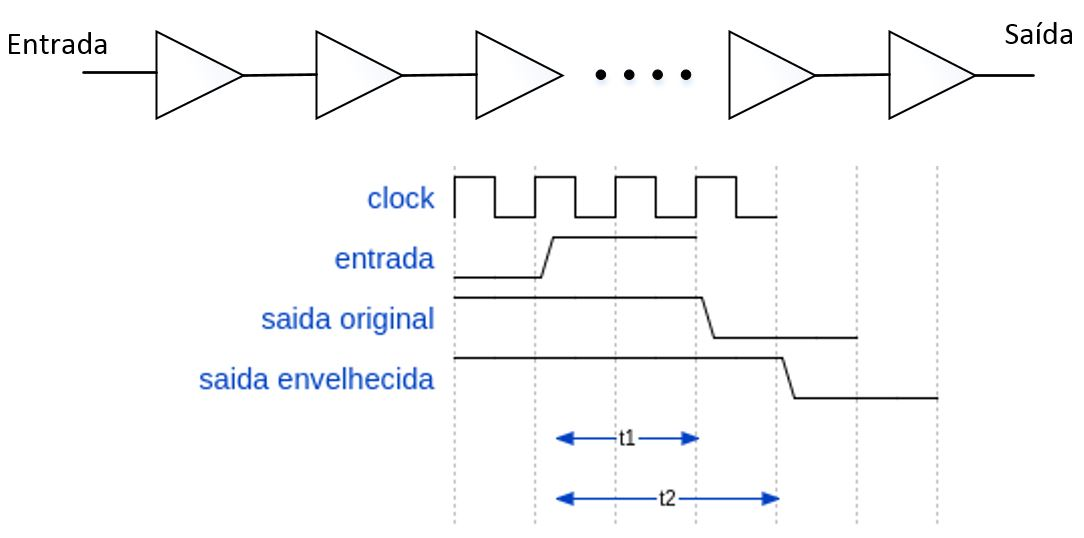
\includegraphics[width=0.8\textwidth]{images/output_delay}
	\caption{Variação no atraso de saída.}
	\label{figure:output_delay}
\end{figure}
Dado um tempo de propagação $t1$ como sendo o tempo necessário para que uma alteração na entrada seja percebida na saída de um circuito não-degradado e caso o tempo de propagação $t2$ medido após um tempo de operação $t_{oper}$ seja maior do que $t1$, este circuito será considerado como envelhecido, conforme exemplo mostrado na figura \ref{figure:output_delay}.

Assim, a variação do atraso de saída é considerada como:
\begin{equation}
\Delta t_d = t2 - t1
\label{eq:variacao_delay_saida}
\end{equation}

Idealmente este atraso de propagação não deveria aumentar. Entretanto, uma variação dele não é um fenômeno inesperado pelos projetistas. Por este motivo, uma salva-guarda (\textit{i.e.} guard-banding)  é planejada a nível de projeto.

Mesmo com esta medida, é possível que a degradação seja tal que extrapole essa salva-guarda. Dessa forma, a variação máxima do atraso $\Delta t_{d,max}$ não pode ultrapassar o \textit{guard-banding}.

\section{Tratamentos dos dados}
\label{section_tratamento_dados}
Os dados obtidos durante a extração de atrasos, MTTF e seus perfis correspondentes são aglutinados e populam o BDPE de forma definitiva. Estes dados compõe a base a ser usada como referência para os métodos descritos na seção \ref{section_metodos_estimativa}.

A formatação específica dessa informações a nível de software fica a critério do projetista. Além disso, o BDPE pode ser modificadp posteriormente para que novos perfis sejam adicionados.

Apesar de a metodologia não ser prejudicada pela existência de entradas duplicadas no banco de dados de perfis envelhecidos, é recomendado que as mesmas sejam únicas. Desta forma, o tamanho do BDPE é reduzido e consequentemente a quantidade de memória necessária para armazená-lo.


% ----------------------------------------------------------
% Results
% ----------------------------------------------------------
\chapter{Resultados}
\epigraph{\textit{Do or do not, there is no try.}}{-Master Yoda}
\label{section:Resultados}
Este capítulo apresenta os resultados das etapas do fluxo proposto, bem como a análise dos mesmos. Alguns resultados preliminares foram utilizados para verificar se o trabalho estava coerente com a base teórica anteriormente exposta. Outros auxiliaram na análise do fluxo de envelhecimento e na acuidade dos métodos de estimativa propostos.

Algumas considerações precisam ser feitas antes da análise dos dados. O ambiente de simulação criado para este trabalho utiliza ferramentas de EAD previamente disponíveis para degradação, sendo sua integração realizada através de um conjunto de \textit{scripts} ou \textit{wrappers}, que são responsáveis por automatizar:
\begin{enumerate}
	\item A criação das diversas netlists utilizadas no fluxo;
	\item Formatação dos arquivos utilizados como banco de dados bem como preenchimento dos mesmos;
	\item A passagem de parâmetros de entrada às ferramentas de EAD;
	\item A extração dos resultados de simulação;
	\item A atualização do banco de dados com os resultados de estimativas de MTTF.
\end{enumerate}

\section{Caracterização de células}
\label{section:caracterização}
Para investigar a relação entre as condições ambientais e a degradação de sistemas, é preciso averiguar primeiramente se é possível reproduzir resultados que estejam coerentes com a literatura. Isso significa que é necessário garantir que, ao se degradar um sistema, as alterações nas condições ambientais (\textit{p.ex.} temperatura) sejam refletidas no sistema conforme esperado. É bem estabelecido que uma alteração na tensão de alimentação $V_{DD}$ e na temperatura deve influenciar não só a operação dos dispositivos mas também na contribuição dos efeitos de degradação expostos na seção \ref{subsection_Conf_CI}. Esta premissa precisa então ser satisfeita.

Com este propósito foram caracterizadas as seguintes células básicas: INV (inversor), AND2, OR2, NOR2 e NAND2. Todas as células foram submetidas a BDPEs estáticos e populados exclusivamente para estas simulações. Por estático indica-se que a célula foi submetida a uma mesma temperatura e tensão ao longo de toda a simulação ao invés de diferentes $T_{conj,X}$ e $V_{conj,Y}$. Cada BDPE possui 200 perfis e o tempo de degradação para todas as células é de 1 ano.

Foram criados 5 BDPE's diferentes, um para cada célula. Entretanto, todos os perfis foram gerados usando a mesma premissa: os valores de temperatura seguem uma distribuição normal de média $\mu = 80$ e desvio-padrão $\sigma=10$. Os valores de tensão também seguem uma distribuição normal, porém de média $\mu = 1.1$ e desvio-padrão $\sigma=0.2$. Foi escolhida uma média de 80$^{\circ}$C com o intuito de garantir uma contribuição significativa da temperatura na degradação. Já a média da tensão de alimentação de $1.1V$ está de acordo com os parâmetros da tecnologia dos transistores utilizados na simulação.

Após cada célula ter sido degradada, o atraso de saída $\Delta t_d$ para cada perfil simulado foi adicionado aos seus respectivos BDPEs e foi criado um modelo de regressão linear múltipla para cada. Os modelos foram utilizados para plotar a dependência do atraso de saída pela tensão de operação e pela temperatura. Os resultados estão representados nas figuras \ref{figure:delays_inv_caracterizacao_200Pontos_gauss80_10} a \ref{figure:delays_or2_caracterizacao_200Pontos_gauss80_10}.
\begin{figure}[H]
\center
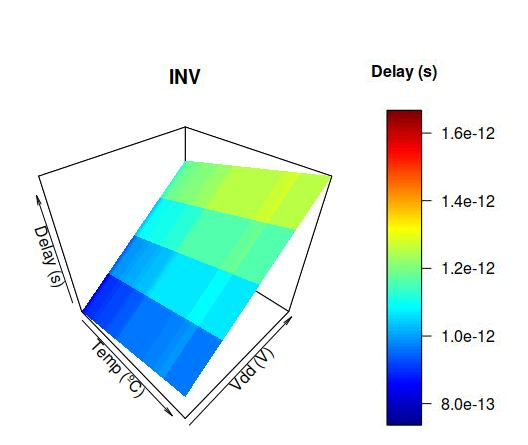
\includegraphics[width=0.6\textwidth]{images/delays_inv_caracterizacao_200Pontos_gauss80_10}
\caption{Caracterização de uma célula inversora degradada durante 1 ano.}
\label{figure:delays_inv_caracterizacao_200Pontos_gauss80_10}	
\end{figure}
A figura \ref{figure:delays_inv_caracterizacao_200Pontos_gauss80_10} mostra que, à medida que a temperatura sobre o inversor (dada em $^{\circ}$C) aumenta, o atraso $\Delta t_d$ (dado em segundos) também incrementa. Entretanto, a influência da temperatura é menor se comparada à da tensão de alimentação, o que era esperado.

Para esta análise, os coeficientes da regressão linear múltipla (e consequentemente a influência de cada grandeza) são dados pelos valores da tabela \ref{tb:regressao_multipla_INV}:
\begin{table}[H]
	\centering
	\caption{Coeficientes do modelo de RLM para o inversor da figura \ref{figure:delays_inv_caracterizacao_200Pontos_gauss80_10}.}
	\begin{tabular}{@{}l|l|l|l@{}}
		\toprule
		& Interceptação & $T_{conj,1}$ & $V_{conj,1}$ \\ \midrule
		Coeficiente & $-1.3049e^{-12}$ & $5.0378e^{-15}$ & $1.9161e^{-12}$ \\ \bottomrule
	\end{tabular}
	\label{tb:regressao_multipla_INV}
\end{table}
Do modelo fica claro que a influência da tensão sobre o envelhecimento é 3 ordens de grandeza maior que a da temperatura. Uma relação semelhante foi encontrada para as células AND2, NAND2, OR2 e NOR2.
\begin{figure}[H]
	\center
	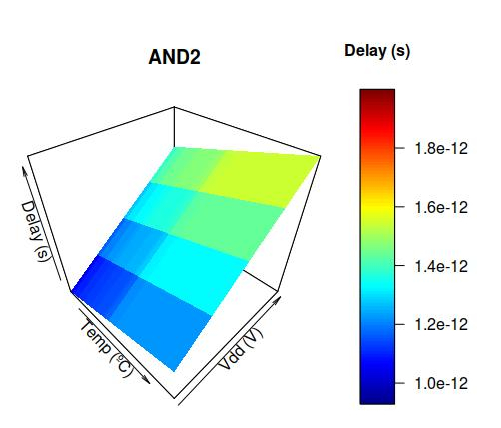
\includegraphics[width=0.6\textwidth]{images/delays_and2_caracterizacao_200Pontos_gauss80_10}
	\caption{Caracterização de uma célula AND2 degradada durante 1 ano.}
	\label{figure:delays_and2_caracterizacao_200Pontos_gauss80_10}	
\end{figure}
\begin{table}[H]
	\centering
	\caption{Coeficientes do modelo de RLM para a figura \ref{figure:delays_and2_caracterizacao_200Pontos_gauss80_10}.}
	\begin{tabular}{@{}l|l|l|l@{}}
		\toprule
		& Interceptação & $T_{conj,1}$ & $V_{conj,1}$ \\ \midrule
		Coeficiente & $-1.4112e^{-12}$ & $5.8058e^{-15}$ & $2.1905e^{-12}$ \\ \bottomrule
	\end{tabular}	
	\label{tb:regressao_multipla_AND2}
\end{table}
\begin{figure}[H]
	\center
	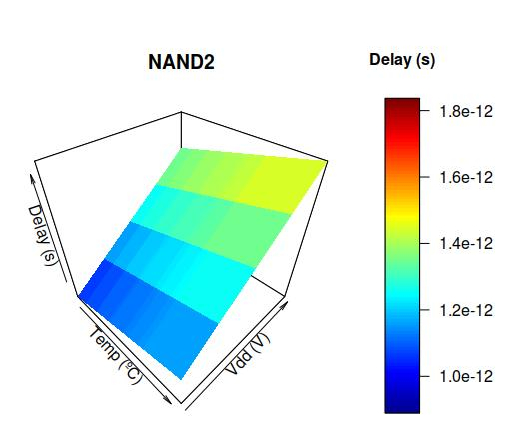
\includegraphics[width=0.6\textwidth]{images/delays_nand2_caracterizacao_200Pontos_gauss80_10}
	\caption{Caracterização de uma célula NAND2 degradada durante 1 ano.}
	\label{figure:delays_nand2_caracterizacao_200Pontos_gauss80_10}	
\end{figure}
\begin{table}[H]
	\centering
	\caption{Coeficientes do modelo de RLM para a figura \ref{figure:delays_nand2_caracterizacao_200Pontos_gauss80_10}.}
	\begin{tabular}{@{}l|l|l|l@{}}
		\toprule
		& Interceptação & $T_{conj,1}$ & $V_{conj,1}$ \\ \midrule
		Coeficiente & $-1.2030e^{-12}$ & $5.5807e^{-15}$ & $1.9283e^{-12}$ \\ \bottomrule
	\end{tabular}
	\label{tb:regressao_multipla_NAND2}
\end{table}
\begin{figure}[H]
	\center
	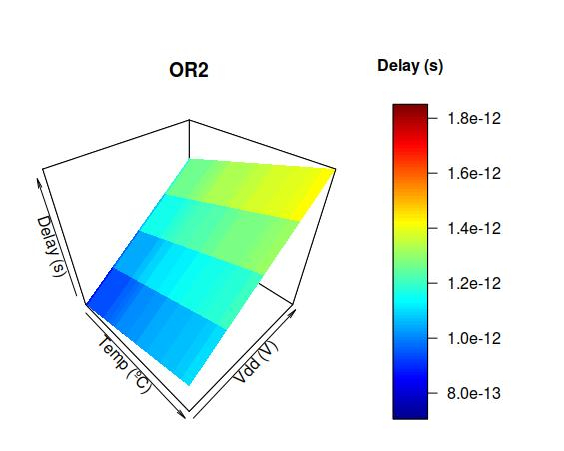
\includegraphics[width=0.6\textwidth]{images/delays_or2_caracterizacao_200Pontos_gauss80_10}
	\caption{Caracterização de uma célula OR2 degradada durante 1 ano.}
	\label{figure:delays_or2_caracterizacao_200Pontos_gauss80_10}	
\end{figure}
\begin{table}[H]
	\centering
	\caption{Coeficientes do modelo de RLM para a figura \ref{figure:delays_or2_caracterizacao_200Pontos_gauss80_10}.}
	\begin{tabular}{@{}l|l|l|l@{}}
		\toprule
		& Interceptação & $T_{conj,1}$ & $V_{conj,1}$ \\ \midrule
		Coeficiente & $-1.5102e^{-12}$ & $5.9055e^{-15}$ & $2.1376e^{-12}$ \\ \bottomrule
	\end{tabular}
	\label{tb:regressao_multipla_OR2}
\end{table}
\begin{figure}[H]
	\center
	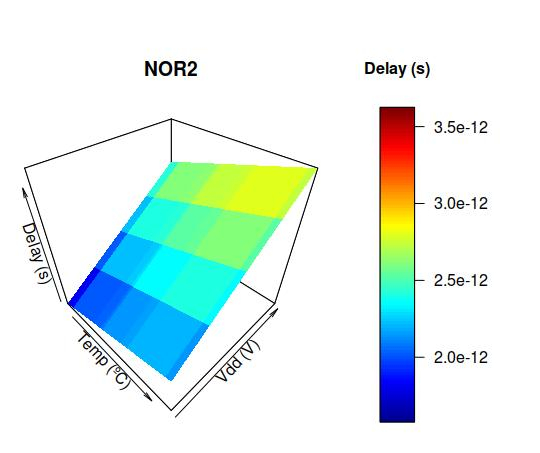
\includegraphics[width=0.6\textwidth]{images/delays_nor2_caracterizacao_200Pontos_gauss80_10}
	\caption{Caracterização de uma célula NOR2 degradada durante 1 ano.}
	\label{figure:delays_nor2_caracterizacao_200Pontos_gauss80_10}	
\end{figure}
\begin{table}[H]
	\centering
	\caption{Coeficientes do modelo de RLM para a figura \ref{figure:delays_or2_caracterizacao_200Pontos_gauss80_10}.}
	\begin{tabular}{@{}l|l|l|l@{}}
		\toprule
		& Interceptação & $T_{conj,1}$ & $V_{conj,1}$ \\ \midrule
		Coeficiente & $-2.9256e^{-12}$ & $1.3332e^{-14}$ & $4.0494^{-12}$ \\ \bottomrule
	\end{tabular}
	\label{tb:regressao_multipla_OR2}
\end{table}

Era esperado que a relação entre tensão de alimentação e atraso fosse positiva. O mesmo pode ser dito entre a temperatura e o atraso. Estes resultados iniciais nos dão segurança de que o fluxo está pronto e que ele pode ser utilizado para sistemas maiores. Além disso, eles confirmam aquilo que já era esperado: quando da utilização do método de correlação, descrito na seção \ref{subsection_estimativas_correlacao}, devemos procurar pelo resultado de maior correlação positiva, já que o atraso cresce com o aumento da temperatura e tensão.
\section{Degradação de circuitos de teste}
\label{section:caracterização_iscas}
Uma vez realizados testes com células básicas, mais circuitos foram utilizados para continuar investigando a viabilidade do fluxo e da metodologia. Com esse intuito, foram utilizados quatro circuitos ISCAS-85: c499, c880, c1355, c5315. Esses circuitos ISCAS são implementações de blocos combinacionais pré-determinados cujo objetivo é propor circuitos padrões para testes de diferentes propósitos \cite{Hansen1999}. A função implementada e a respectiva quantidade de portas lógicas para cada um deles está descrita na tabela \ref{tb:ISCAS_85}.

\begin{table}[H]
\centering
\caption{Características da cadeia de inversores e dos circuitos ISCAS-85 utilizados \cite{Hansen1999}.}
\begin{tabular}{@{}lll@{}}
\toprule
Circuito & Função & Qtde. de portas \\ \midrule
inv100 & Cadeia de Inversores & \ \ \ \ 100 \\ \midrule
c499 & Single-Error-Correcting de 32-bit & \ \ \ \ 474 \\ \midrule
c880 & ULA de 8 bits & \ \ \ \ 393 \\ \midrule
c1355 & Single-Error-Correcting de 32-bit & \ \ \ \ 738 \\ \midrule
c5315 & ULA de 9 bits & \ \ \ \ 1781 \\ \bottomrule
\end{tabular}
\label{tb:ISCAS_85}
\end{table}
Esses circuitos podem ser utilizados para os próximos passos em sua integridade ou apenas uma porção dos mesmos. Por integridade entende-se que os circuitos, inicialmente descritos através de uma linguagem de descrição de hardware (Hardware Description Language, HDL), serão sintetizados e uma netlist esquemática no formato Spectre criada. 

Por porção entende-se que somente uma parte do circuito será utilizada para criação da netlist Spectre. Esta parte deve ser capaz de, após as simulações de degradação, representar o pior caso para o restante do circuito. Esta porção pode ser representada por um ou mais caminhos críticos, conforme exposto na seção \ref{section_extracao_caminhos}.
Foram extraídos os caminhos críticos dos circuitos ISCAS da tabela \ref{tb:ISCAS_85} e netlists esquemáticas menores foram criadas a partir destes caminhos.

Para extração dessa informação, foi utilizada uma funcionalidade nativa da ferramenta de síntese capaz de relatar quais são os caminhos críticos de um circuito. Além disso, eles devem ser ativados de tal forma que uma transição na saída seja detectável. Isso significa que as portas lógicas serão ativadas ou desativadas em uma combinação específica que reflita não só o maior atraso de propagação possível mas também uma mudança lógica na saída do caminho crítico.

Após a extração destes caminhos, os circuitos foram reduzidos aos tamanhos descritos na tabela \ref{tb:tamanho_piores_caminhos}.
\begin{table}[H]
	\centering
	\caption{Tamanho dos circuitos de teste após a extração dos caminhos críticos.}
	\begin{tabular}{@{}ll@{}}
		\toprule
		Circuito & Qtde. de portas \\ \midrule
		inv100 & \ \ \ \ 100 \\ \midrule
		w\_c499 & \ \ \ \ 10 \\ \midrule
		w\_c880 & \ \ \ \ 8 \\ \midrule
		w\_c1355 & \ \ \ \ 21 \\ \midrule
		w\_c5315 & \ \ \ \ 25 \\ \bottomrule
	\end{tabular}
	\label{tb:tamanho_piores_caminhos}
\end{table}
O sufixo ``w\_'' foi adicionado aos nomes dos ISCAS unicamente como forma de diferenciar os circuitos com caminhos críticos (\textit{p. ex.} w\_c499) dos seus respectivos circuitos completos. Após a extração dos caminhos, um circuito de teste (\textit{testbench}) foi criado para cada um dos circuitos da tabela \ref{tb:tamanho_piores_caminhos} cujo objetivo é ativar o caminho crítico, conforme mencionado anteriormente.  

Uma vez criadas, as netlists são padronizadas com valores de temperatura $T=0$ e alimentação $V_{DD}=0.0$. Eles são utilizados como referência pelos \textit{scripts}, substituindo estes valores pelos respectivos $T_{conj,X}$ e $V_{conj,Y}$ durante a simulação.

Como exemplo, considere que a tabela \ref{tb:regressao_multipla_exemplo2} possui perfis de envelhecimento para o circuito $w\_c499$. Para o primeiro perfil, serão criadas $N=14$ netlists, das quais 13 serão submetidas a uma temperatura $T=30^{\circ}C$ e uma a $T=50^{\circ}C$. Já para $V_{DD}$, 12 estarão submetidas a uma tensão $V_{DD}=1.0V$ e duas a $V_{DD}=1.1V$. Dessa forma, as 12 primeiras netlists terão os valores $T=0$ e $V_{DD}=0.0$ substituídos por $T=30^{\circ}C$ e alimentação $V_{DD}=1.0V$. A 13º netlist terá $T=30^{\circ}C$ e $V_{DD}=1.1V$. A restante terá $T=50^{\circ}C$ e $V_{DD}=1.1V$.

Cada circuito foi submetido a um BDPE de aproximadamente 250 entradas cujos perfis são submetidos aos conjuntos de condições ambientais $T_{conj,X}=[10, 30, 50, 70, 90]$ e $V_{conj,Y}=[0.9, 1.0, 1.1, 1.2, 1.3]$. Os valores de $p_{T(w,x)}$ e $p_{V(w,y)}$ foram gerados pseudo-aleatoriamente, sendo $\sum p_{T(w,x)}=100$ e $\sum p_{V(w,y)}=100$ (ou seja, $N=100$). Assim sendo, cada entrada do BDPE corresponde a 100 degradações, totalizando 2500 simulações de envelhecimento para toda o banco de dados de perfis e que são posteriormente adicionados ao BDPE, conforme descrito no capítulo 4.

Uma segunda bateria de testes é realizada, porém com condições ambientais diferentes. Os mesmos circuitos são degradados mas desta vez submetidos a um BDPE estático. Isso significa que o perfil ao qual são submetidos permanece 100\% do tempo em um único $T_{conj,X}$ e um único $V_{conj,Y}$. Esse comportamento é representado através da criação de uma tabela de perfis, representada na tabela \ref{tb:BDPE_estatico}.

\begin{table}[H]
	\centering
	\caption{BDPE estático utilizado no envelhecimento dos circuitos de teste.}
	\begin{tabular}{@{}l|l|l|l|l|l@{}}
		\toprule
		$40$ & $70$ & $100$ & $1.0$ & $1.1$ & $1.2$ \\ \midrule
		$3$ & $0$ & $0$ & $3$ & $0$ & $0$ \\
		$0$ & $3$ & $0$ & $3$ & $0$ & $0$ \\
		$0$ & $0$ & $3$ & $3$ & $0$ & $0$ \\
		$3$ & $0$ & $0$ & $0$ & $3$ & $0$ \\
		$0$ & $3$ & $0$ & $0$ & $3$ & $0$ \\
		$0$ & $0$ & $3$ & $0$ & $3$ & $0$ \\
		$3$ & $0$ & $0$ & $0$ & $0$ & $3$ \\
		$0$ & $3$ & $0$ & $0$ & $0$ & $3$ \\
		$0$ & $0$ & $3$ & $0$ & $0$ & $3$ \\
		\bottomrule
	\end{tabular}
	\label{tb:BDPE_estatico}
\end{table}
Este tipo de teste auxilia a investigar melhor quais são as vantagens da metodologia proposta ao comparar os resultados anteriores com os de uma abordagem de perfis estáticos. É preciso esclarecer primeiramente que um perfil definido por $T_{conj,X}=[40,70,100]$ e $p_{T(1,x)}=[3,0,0]$, utilizando a tabela \ref{tb:BDPE_estatico} como exemplo, não necessariamente indica que um sistema foi degradado sob influência de uma temperatura e tensão constantes. Para um sistema real não é possível assumir essa premissa. Entretanto, o perfil de temperatura e tensão podem, por escolha do projetista, ser representados por médias (\textit{p.ex} temperatura média ou tensão de alimentação média).

Dessa forma, é possível avaliar se a representação estática da operação do sistema oferece uma precisão semelhante à representação dinâmica. Se for possível representar o perfil de um sistema através de uma estatística simples (como as médias) e obter um erro de predição semelhante ou melhor do que a dinâmica, então deve-se questionar a utilização de um BDPE dinâmico, já que não existiria, em tese, uma redução do erro. Esta análise também será realizada nas seções subsequentes.
\section{Métricas e estatísticas}
\label{section:metricas_estatisticas}
Antes de explorar os dados de simulação, é preciso explicar quais métricas foram utilizadas para este trabalho. Uma métrica, no contexto aqui apresentado, deve ser capaz de indicar a precisão ou assertividade dos métodos de estimativa apresentados na seção \ref{section_metodos_estimativa}, dando uma perspectiva diferenciada dos resultados. Qual métrica se mostra mais adequada é um debate que não faz parte deste trabalho, visto que não há consenso na literatura específica da área \cite{Poli1993}\cite{Willmott}\cite{Chai2014}. Ao invés disso, mais de uma métrica será utilizada, cabendo ao projetista julgar a mais adequada ao entendimento de seus dados.

A análise gráfica dos resultados utilizará apenas algumas destas métricas. Entretanto serão sumarizadas, ao longo da análise, as seguintes métricas: Erro Relativo (ER), Erro Máximo (EMAX), Erro Quadrático Médio (EQM) e Erro Normalizado da Raiz do Valor Quadrático Médio (ENRVQM). Estas métricas são expressas por:
\begin{align}
ER = 100\left(1 - \frac{\hat{y_i}}{y_i}\right) \\
EMAX = \max{\left(100\left(1 - \frac{\hat{y_i}}{y_i}\right)\right)} \\
EQM = \frac{\sum_{i=1}^{n}(\hat{y_i}-y_i)^2}{n} \\
ENRVQM = \frac{\sqrt{EQM}}{\bar{y}}
\end{align}
onde $n$ representa a quantidade de observações, $\bar{y}$ é a média dos dados observados, $\hat{y_i}$ é o i-ésimo dado observado e $y_i$ o i-ésimo dado estimado.
Por ser a mais simples e intuitiva, o ER é a primeira métrica a ser explorada adiante.

Apesar de dispormos destas essas métricas, é interesse evitar que um modelo de estimativa não sofra com um efeito de sobreajuste, ou seja, ele tente se acomodar demasiadamente aos dados observados, reduzindo a performance do modelo e consequentemente afetando as métricas mencionadas acima.

Para evitar o sobreajuste, foi utilizado uma técnica de validação cruzada. Esta abordagem propõe dividir os dados pré-existentes em dois grupos: dados de treino e dados de teste. Os dados de treinamento são utilizados para obtenção do modelo preditivo. Já os dados de teste são utilizados para medir a precisão do modelo. A técnica de validação cruzada escolhida para a análise foi \textit{leave-one-out cross-validation} (LOOCV), onde apenas uma das amostras é utilizada como teste e as restantes são utilizadas como dados de treino \cite{James2013}.

Utilizemos a tabela \ref{tb:exemplo_cross_validation}, que é um excerto de um dos BDPE utilizados neste trabalho, como exemplo.  
\begin{table}[H]
	\centering
	\caption{Excerto de um BDPE com dados de simulação.}
	\begin{tabular}{@{}l|l|l|l|l|l|l|l|l|l|l@{}}
		\toprule
		$10$ & $30$ & $50$ & $70$ & $90$ & $0.9$ & $1.0$ & $1.1$ & $1.2$ & $1.3$ & MTTF \\ \midrule
		$37$ & $56$ & $1$ & $6$ & $0$ & $37$ & $56$ & $1$ & $6$ & $0$ & $1.46$ \\
		$70$ & $0$ & $7$ & $0$ & $23$ & $70$ & $0$ & $7$ & $0$ & $23$ & $1.13$ \\
		$47$ & $0$ & $0$ & $42$ & $11$ & $47$ & $0$ & $0$ & $42$ & $11$ & $1.15$ \\
		\bottomrule
	\end{tabular}
	\label{tb:exemplo_cross_validation}
\end{table}
Na técnica de LOOCV a primeira amostra (linha 2 da tabela \ref{tb:exemplo_cross_validation}) é retirada, por exemplo, restando somente 2 entradas para criação do modelo preditivo, seja ele PLS-R, DE ou COR. Após criado, a amostra retirada é usada como entrada no modelo e o resultado estimado $\hat{y_1}$ é comparado ao esperado $y_1$. Nesse exemplo, considerando um tempo de operação $t_{oper}=1$ ano, é conhecido que, para um perfil $p_{T(1,x)}=[37,56,1,6,0]$ e $p_{V(1,y)}=[37,56,1,6,0]$, o resultado esperado é $y_1=1.46$ (MTTF de 1.46 anos). A partir daí, as métricas de erro anteriormente mencionadas podem se utilizadas para medir a precisão dos métodos.

Para se obter métricas mais significativas ainda, a LOOCV foi utilizada $N$ vezes, onde $N$ é quantidade de amostras do BDPE. Isso significa que, após a primeira amostra ser utilizada como teste e os erros serem calculados, a LOOCV é repetida mas desta vez usando a segunda amostra como teste e assim sucessivamente. Todos os resultados são utilizados para compor as métricas mencionadas. Dessa forma não se está testando um modelo específico obtido através de um método de distância euclideana, por exemplo, mas está sendo testado ``exaustivamente'' a DE como método de estimativa.

É importante salientar que durante a operação real do sistema, ao contrário do ambiente de simulação, o modelo já será conhecido no momento em que a predição for necessária, pois já foi previamente treinado. O perfil que é utilizado na análise \textit{online} como entrada para o modelo é proveniente do BDM (e não do BDPE).
\section{Resultados das simulações dos circuitos de teste}
A primeira métrica analisada foi o erro relativo, como forma de compreender a exatidão dos métodos. Levando em consideração que o ``verdadeiro'' valor do MTTF é conhecido, o erro relativo em valores absolutos para o BDPE descrito na seção \ref{section:caracterização_iscas} é representado pelos diagramas de caixa das figuras \ref{figure:ER_MTTF} e \ref{figure:erro_relativo_MTTF_inv100_random}.
\begin{figure}[H]
	\subfloat[ER para pior caminho do ISCAS c499\label{figure:erro_relativo_MTTF_worst_c499_random2}]{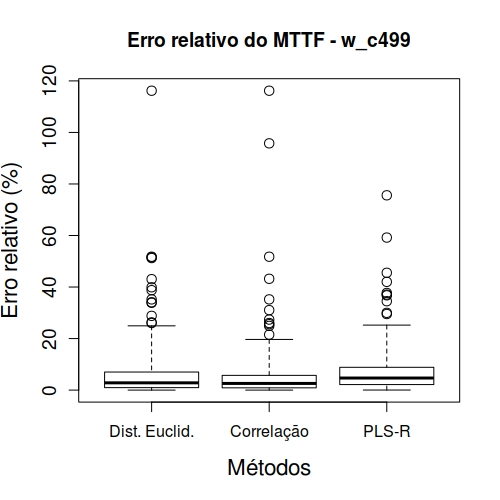
\includegraphics[width=0.5\textwidth]{images/erro_relativo_MTTF_worst_c499_random2}
	}
	\hfill
	\subfloat[ER para pior caminho do ISCAS c880\label{figure:erro_relativo_MTTF_worst_c880_random2}]{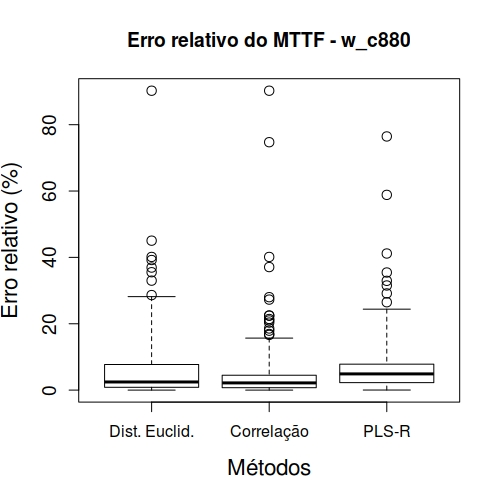
\includegraphics[width=0.5\textwidth]{images/erro_relativo_MTTF_worst_c880_random2}
	}
	\hfill
	\subfloat[ER para pior caminho do ISCAS c1355\label{figure:erro_relativo_MTTF_worst_c1355_random2}]{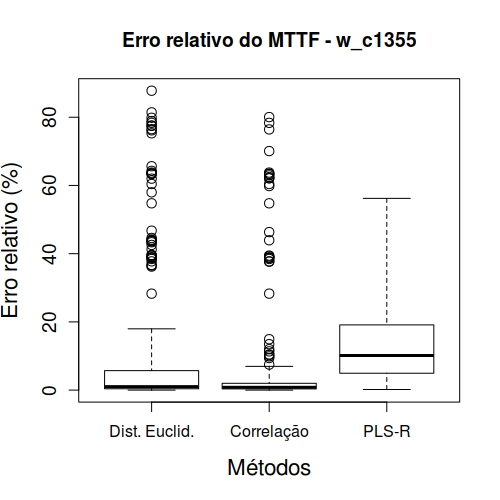
\includegraphics[width=0.5\textwidth]{images/erro_relativo_MTTF_worst_c1355_random2}
	}
	\hfill
	\subfloat[ER para pior caminho do ISCAS c5315\label{figure:erro_relativo_MTTF_worst_c5315_random2}]{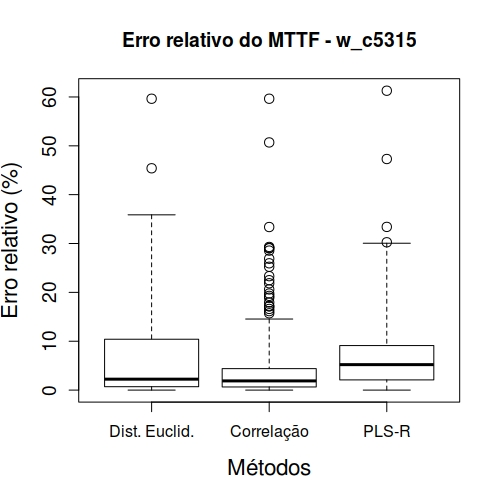
\includegraphics[width=0.5\textwidth]{images/erro_relativo_MTTF_worst_c5315_random2}
	}
	\caption{Erro relativo do MTTF para os circuitos ISCAS-85.}
	\label{figure:ER_MTTF}
\end{figure}
\begin{figure}[H]
	\center
	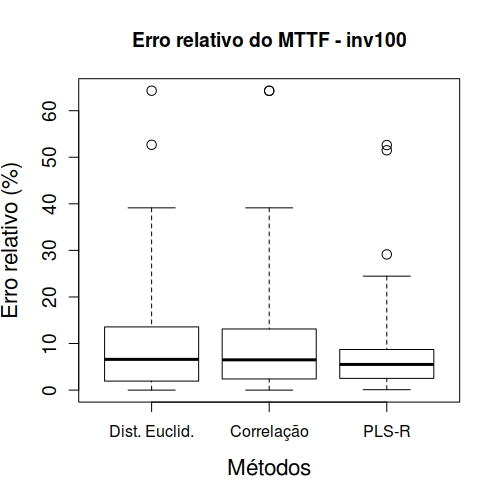
\includegraphics[width=0.5\textwidth]{images/erro_relativo_MTTF_inv100_random}
	\caption{Erro relativo do MTTF para a cadeia de inversores.}
	\label{figure:erro_relativo_MTTF_inv100_random}	
\end{figure}

Extraindo o EMAX (como uma porcentagem) para cada circuito e método obtém-se:

\begin{table}[H]
	\centering
	\caption{Erro máximo para os circuitos de teste.}
	\begin{tabular}{@{}l|l|l|l@{}}
		\toprule
		Circuito & Dist. Eucli. & Cor. & PLS-R \\ \midrule
		inv100 & \ \ \ 64.29\% & 64.29\% & 52.61\% \\
		w\_c499 & \ \ \ 116.21\% & 116.21\% & 75.61\% \\
		w\_c880 &  \ \ \ 90.24\% & 90.24\% & 76.45\% \\
		w\_c1355 & \ \ \ 80.05\% & 87.78\% & 56.21\% \\
		w\_c5315 & \ \ \ 59.64\% & 59.64\% & 61.28\% \\
		\bottomrule
	\end{tabular}
	\label{tb:erro_maximo_ISCAS}
\end{table}

Para obter uma comparação mais intuitiva, o Erro Quadrático Médio (EQM) foi calculado para cada um dos circuitos e por fim normalizado, servindo como um rápido indicativo de qual método é mais preciso e o quão mais preciso é em comparação aos demais. 
\begin{figure}[H]
	\subfloat[EQMN para pior caminho do ISCAS c499\label{figure:NMSE_MTTF_worst_c499_random2}]{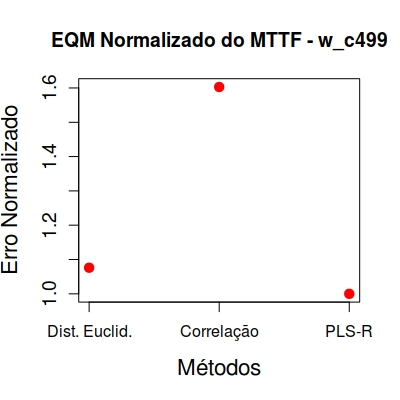
\includegraphics[width=0.5\textwidth]{images/NMSE_MTTF_worst_c499_random2}
	}
	\hfill
	\subfloat[EQMN para pior caminho do ISCAS c880\label{figure:NMSE_MTTF_worst_c880_random2}]{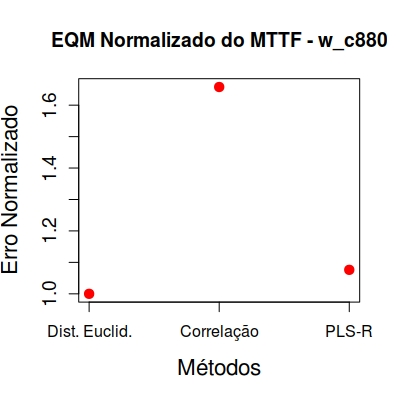
\includegraphics[width=0.5\textwidth]{images/NMSE_MTTF_worst_c880_random2}
	}
	\hfill
	\subfloat[EQMN para pior caminho do ISCAS c1355\label{figure:NMSE_MTTF_worst_c1355_random2}]{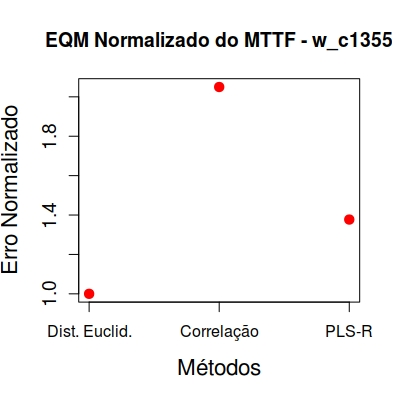
\includegraphics[width=0.5\textwidth]{images/NMSE_MTTF_worst_c1355_random2}
	}
	\hfill
	\subfloat[EQMN para pior caminho do ISCAS c5315\label{figure:NMSE_MTTF_worst_c5315_random2}]{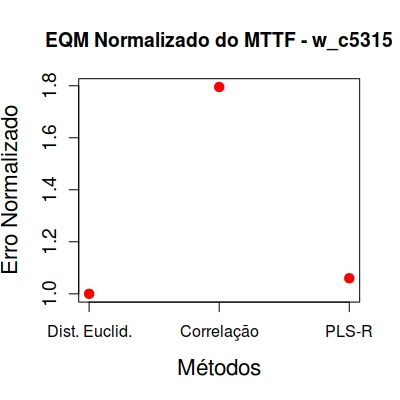
\includegraphics[width=0.5\textwidth]{images/NMSE_MTTF_worst_c5315_random2}
	}
	\caption{Erro Quadrático Médio Normalizado do MTTF para os circuitos ISCAS-85.}
	\label{figure:NMSE_MTTF}
\end{figure}
\begin{figure}[H]
	\center
	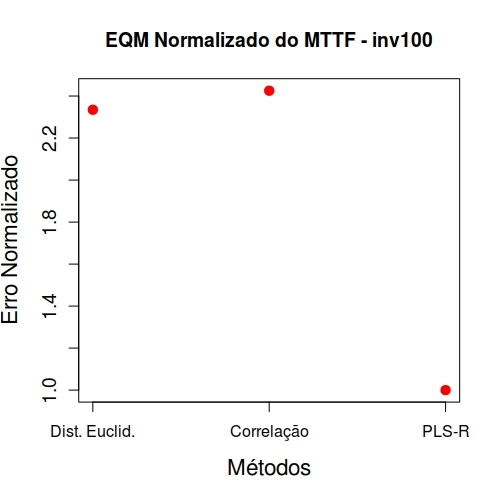
\includegraphics[width=0.5\textwidth]{images/NMSE_MTTF_inv100_random}
	\caption{Erro Quadrático Médio Normalizado do MTTF para a cadeia de inversores.}
	\label{figure:NMSE_MTTF_inv100_random}	
\end{figure}

Entretanto, ao se analisar circuitos de diferentes dimensões, e consequentemente conjuntos de dados de diferença expressiva, algumas das métricas obtidas podem estar em escalas diferentes umas das outras, dificultando a compreensão da precisão dos métodos. Nestes casos, o Erro Normalizado da Raiz do Valor Quadrático Médio facilita a interpretação pois cada conjunto de dados é normalizado pela sua própria média, resultando em um erro percentual. Esse é o caso para a simulação da cadeia de inversores. Sendo substancialmente maior que os demais (de 4 a 10 vezes), seu atraso também é maior e a grandeza, nesse caso, maior. 

O ENRVQM foi extraído para cada circuito e método e estão descritos na tabela \ref{tb:ENRVQM}.

\begin{table}[H]
	\centering
	\caption{Erro Normalizado da Raiz do Valor Quadrático Médio para cada método e circuito em \%.}
	\begin{tabular}{@{}l|l|l|l@{}}
		\toprule
		Circuito & Dist. Eucli. & Cor. & PLS-R \\ \midrule
		inv100 & \ \ \ 13.0\% & 13.1\% & 9.1\% \\
		w\_c499 & \ \ \ 8.1\% & 10.1\% & 8.3\% \\
		w\_c880 &  \ \ \ 7.3\% & 9.6\% & 7.9\% \\
		w\_c1355 & \ \ \ 13.5\% & 18.1\% & 14.7\% \\
		w\_c5315 & \ \ \ 7.9\% & 10.6\% & 8.1\% \\
		\bottomrule
	\end{tabular}
	\label{tb:ENRVQM}
\end{table}

Em seguida foram realizadas simulações de degradação para o BDPE estático mencionada na seção \ref{section:caracterização_iscas} e representado na tabela \ref{tb:BDPE_estatico}. O Erro Normalizado da Raiz do Valor Quadrático Médio para os perfis estáticos se encontram na tabela \ref{tb:ENRVQM_estatico}.
\begin{table}[H]
	\centering
	\caption{ENRVQM para cada método e circuito submetidos à perfis estáticos em \%.}
	\begin{tabular}{@{}l|l|l|l@{}}
		\toprule
		Circuito & Dist. Eucli. & Cor. & PLS-R \\ \midrule
		inv100 & \ \ \ 18.08\% & 18.08\% & 2.07\% \\
		w\_c499 & \ \ \ 22.12\% & 22.12\% & 2.55\% \\
		w\_c880 &  \ \ \ 14.79\% & 14.79\% & 3.00\% \\
		w\_c1355 & \ \ \ 29.76\% & 29.76\% & 4.85\% \\
		w\_c5315 & \ \ \ 15.85\% & 15.85\% & 3.44\% \\
		\bottomrule
	\end{tabular}
	\label{tb:ENRVQM_estatico}
\end{table}

\section{Discussão dos resultados}
Ao se analisar o Erro Relativo (ER) através do diagrama de caixas fica subentendido, inicialmente, que a COR e a DE são métodos mais apropriados. A mediana de ambos os métodos é muito próxima de $0$. Isso é um indicativo de que o ER é muito pequeno em muitos casos. Além disso, a COR parece ser o melhor dos métodos, visto que 75\% dos seus erros relativos estão ``comprimidos'' na região de $ER=0$. 

Entretanto, a quantidade de \textit{outliers} aparenta ser alta. Se a ocorrência de outliers for considerável, isso se refletirá negativamente na precisão dos métodos. Observando a tabela \ref{tb:erro_maximo_ISCAS}, o EMAX dos métodos indica que, quando existe um erro na previsão, ele pode ser de aproximadamente 100\%. Isso significa que o dado estimado $\hat{y_i}$ é até duas vezes maior (ou duas vezes menor) que o ${y_i}$ esperado.

Logo, é preciso averiguar se esses grandes erros de estimativa são usuais para os métodos e dados observados. Se forem, o erro quadrático médio é capaz de enfatizar estes erros. Porém, ao se trabalhar com métricas quadráticas, o resultado não mantém um significado físico plausível. Por este motivo, o resultado é normalizado (EQMN) utilizando o menor erro como referência e apresentado como mostrado na figura \ref{figure:NMSE_MTTF} para facilitar a compreensão.

O EQMN deixa explícito que a Distância Euclideana não é um método tão impreciso quanto indicava o diagrama de caixas do ER. Em adição, a PLS-R mostra-se como um método de precisão comparável à DE. Já a correlação está se mostrando como sendo o pior dos métodos entre os três, sendo até duas vezes mais impreciso que a DE.

Como mencionado na seção \ref{section:metricas_estatisticas}, não há consenso na literatura sobre qual métrica é a mais apropriada para análise de erros de estimativas. Por isso, além do Erro Quadrático Médio, o Erro Normalizado da Raiz do Valor Quadrático Médio também é utilizado, podendo ajudar a compreender um pouco melhor os resultados obtidos. Assim como a figura \ref{figure:NMSE_MTTF}, a tabela \ref{tb:ENRVQM} também indica que a DE e a PLS-R possuem uma precisão semelhante. Entretanto, o ENRVQM médio para DE é de $10\%$ e de $9.6\%$ para a Regressão de Mínimos Quadrados Parciais. Já a Correlação apresenta um ENRVQM médio de $12.3\%$ e consolida-se como o pior método para estimativa.

Esses resultados mostram que uma estratégia proativa para extensão do tempo de vida de um sistema que utilize a Distância Euclideana ou PLS-R como método de estimativa pode ter uma precisão de aproximadamente 90\%. Esta performance pode ser melhorada ainda mais à medida que o BDPE for atualizado com dados de campo. A metodologia, ao propor uma modularização do sistema (conforme descrito na seção \ref{section_visao_geral}) permite que os próprios modelos sejam atualizados ou substituídos, potencialmente melhorando ainda mais a precisão.

Ao repetirmos esta análise para um BDPE estático, a tabela \ref{tb:ENRVQM_estatico} evidencia que o Erro Normalizado da Raiz do Valor Quadrático Médio para a DE e COR piora bastante. Não é surpreendente um banco que possui poucas entradas, e um espaço amostral tão baixo, afetar estes dois métodos. Ao calcular-se a DE, por exemplo, a distância obtida será igual em todos os casos. Assim, qualquer um dos perfis pode ser enquadrado na condição de ``mais próximo'', o que não é satisfatório.

Adicionalmente, o ENRVQM para a PLS-R mostra-se muito melhor. Observando-se as três primeiras linhas da tabela \ref{tb:BDPE_estatico}, é  possível perceber que a tensão de alimentação mantém-se a mesma, enquanto a temperatura pode apresentar apenas os valores de 40, 70 e 100. O mesmo pode ser observado para o restante dos dados. Separando estas informações em grupos que possuem a mesma tensão de alimentação, a dependência do atraso de saída pela temperatura para diferentes $V_{DD}$ é dada pela figura \ref{figure:Temp_atraso_VDDcte}.
\begin{figure}[H]
	\center
	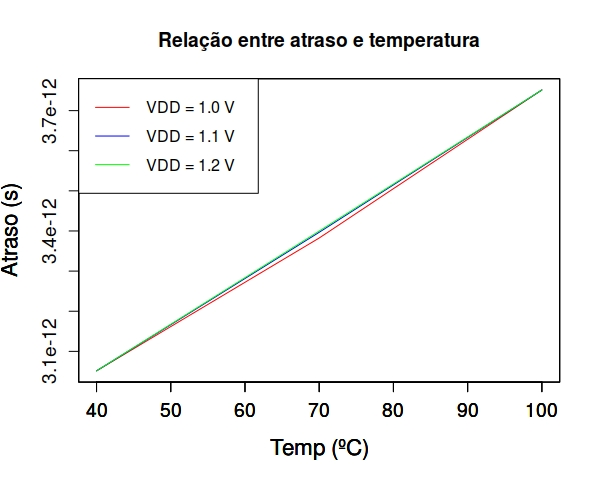
\includegraphics[width=0.8\textwidth]{images/Temp_atraso_VDDcte}
	\caption{Relação entre o atraso e a temperatura para diferentes $V_{DD}$.}
	\label{figure:Temp_atraso_VDDcte}	
\end{figure}

A decomposição dos dados exposta na figura \ref{figure:Temp_atraso_VDDcte} possui uma serventia didática apenas, pois facilita visualizar a relação linear existente entre temperatura e atraso (e consequentemente MTTF). Similarmente, o mesmo pode ser feito entre a tensão de alimentação e o atraso. Se há uma relação linear tão evidente entre estas variáveis explicativas (Temperatura e Tensão) e a variável observada (Atraso ou MTTF), o modelo de PLS-R extraído será consequentemente bem mais preciso.

Este é o motivo pelo qual o ENRVQM para um BDPE estático é mais preciso do que para um BDPE dinâmico. É necessário ressaltar que o um banco de dados de perfis estático considera uma estatística (possivelmente média) para as condições ambientais, sendo bem menos fiel ao verdadeiro perfil de operação de um sistema.

\section{Críticas ao método}
O método apresentado propõe a utilização de diferentes unidades para realizar a tarefa de predição, conforme mostrado na figura \ref{figure:sistema_proposta_metodologia}. Apesar de essa abordagem se mostrar como uma vantagem, permitindo que suas diversas unidades sejam customizadas, melhoradas ou mesmo completamente substituídas, alguns de seus aspectos não estão bem definidos.

Não está definido, por exemplo, se existe uma dimensão recomendada para o BDPE dinâmico. Na análise realizada foram utilizados aproximadamente 250 perfis. Não há entretanto uma motivação específica. Usualmente 30 ou mais amostras são mais do que suficientes para que a distribuição amostral da média de uma população seja considerada uma distribuição \textit{gaussiana} \cite{Montgomery2011}. Entretanto, uma quantidade inferior não garante que a distribuição da estatística será ``não-normal''.

No contexto desse trabalho, essa estatística pode ser o acréscimo médio no atraso $t_d$ ou o MTTF médio. Independente de qual estatística seja escolhida pode-se realizar a análise de um BDPE dinâmico reduzido, com uma quantidade de amostras inferiores e averiguar como os métodos se comportam. Após repetir esta análise com apenas 28 perfis, evitando a garantia de normalidade da média, o ENRVQM obtido para os circuitos e métodos é apresentado na tabela \ref{tb:ENRVQM_reduzido}.

\begin{table}[H]
	\centering
	\caption{ENRVQM para cada método e circuito submetidos à 28 perfis dinâmicos.}
	\begin{tabular}{@{}l|l|l|l@{}}
		\toprule
		Circuito & Dist. Eucli. & Cor. & PLS-R \\ \midrule
		inv100 & \ \ \ 14.89\% & 15.89\% & 7.61\% \\
		w\_c499 & \ \ \ 21.99\% & 26.13\% & 9.21\% \\
		w\_c880 &  \ \ \ 21.25\% & 22.55\% & 8.87\% \\
		w\_c1355 & \ \ \ 14.23\% & 16.49\% & 14.86\% \\
		w\_c5315 & \ \ \ 17.99\% & 19.41\% & 8.95\% \\
		\bottomrule
	\end{tabular}
	\label{tb:ENRVQM_reduzido}
\end{table}

O ENRVQM médio para a DE é de 18.07\% e para a PLS-R é de 9.9\%. Para a COR é obtido um ENRVQM médio de 20.09\%. Apesar de a PLS-R se manter como o melhor método, a diferença para a DE é considerável desta vez. Então a crítica ao método se mantém e levanta alguns questionamentos:
\begin{enumerate}
	\item Qual é a dimensão do BDPE necessária para que se tenha uma boa predição?
	\item Aumentar o BDPE ainda mais garantirá que a DE se torne um método melhor que a PLS-R eventualmente?
	\item Qual é a relação existente entre o aumento do BDPE e a redução dos erros de predição para cada método?
\end{enumerate}
% ----------------------------------------------------------
% Conclusions
% ----------------------------------------------------------
\chapter{Conclusões}
Estimar o tempo de vida de sistemas integrados é imperativo diante do atual avanço tecnológico e do consequente estresse submetido a eles. Efeitos físicos antes ignorados, agora passam a contribuir de forma preponderante para a degradação de circuitos integrados.

Nesse contexto surge a necessidade de observar, investigar e adequar a operação de um sistema afim de mitigar ou reduzir o desgaste decorrente de um perfil de operação. Inúmeras técnicas foram desenvolvidas e estão disponíveis na literatura que permitem coletar informações de diferentes origens e interpretá-las.

A metodologia aqui proposta permite integrar a coleta destes dados, ao mesmo tempo que representa estas informações na forma de perfis de operações. Não apenas isso, mas a metodologia está pronta para simular, degradar e estimar o tempo de vida restante de sistemas.

Apresentando uma abordagem que independe da origem dos dados e das técnicas já existentes, este trabalho permite que o projetista adeque o fluxo às suas necessidades; seja otimizando os métodos preditivos aqui propostos, seja utilizando outros inteiramente diferentes. Além disso, o trabalho independe da tecnologia utilizada no sensoriamento dos parâmetros de operação, do nó tecnológico ou até mesmo da variação sofrida no processo de fabricação dos dispositivos.

Circuitos de teste foram degradados como prova de conceito, mostrando que modelos preditivos menos complexos são capazes de estimar o MTTF com uma precisão de aproximadamente 90\% no melhor dos casos. Em adição, um banco de dados que represente estaticamente as condições ambientais de operação de um sistema não se mostra realístico.

\section{Futuros trabalhos}
Trabalhos futuros envolvem a automatização completa de todo o processo de extração de caminhos críticos, síntese e representação esquemática.

Abordagens diferentes de aprendizado de máquina (\textit{p.ex.} redes neurais), podem ser utilizadas e comparadas aos métodos utilizados, averiguando o impacto na área, consumo e precisão das estimativas. Além disso, a metodologia pode ser melhorada para que seja possível modelar o BDPE em função do número de amostras e métodos de estimativa utilizados, permitindo ao projetista analisar o \textit{trade-off} entre precisão, área ocupada pelo BDPE e métodos escolhidos.

% ----------------------------------------------------------
% ELEMENTOS PÓS-TEXTUAIS
% ----------------------------------------------------------
\postextual
% ----------------------------------------------------------

% ----------------------------------------------------------
% Referências bibliográficas
% ----------------------------------------------------------
\bibliography{bibliografia}


% ----------------------------------------------------------
% Glossário
% ----------------------------------------------------------
%
% Consulte o manual da classe abntex2 para orientações sobre o glossário.
%
%\glossary

% ----------------------------------------------------------
% Apêndices
% ----------------------------------------------------------

% ---
% Inicia os apêndices
% ---
% \begin{apendicesenv}
% 
% % Imprime uma página indicando o início dos apêndices
% \partapendices
% 
% % ----------------------------------------------------------
% \chapter{Analyzed QCA Structures}
% \label{Appendix_Analyzed_QCA_Structures}
% 
\section{Wire}
%%%%%%%%%%%%%%%%%%%%%%%%%%%%%%%%%%%%%%%%%%%%%%%%%%%%%%%%%%%%%%%%%%%%%%%%%%%%%%%%%%%%%%%%%%%%%%%%%%%%%%%%%%%%%%%%%%%%%%%%%
\flushleft
\begin{tabular}[l]{c c}
  WIR1 - Regular & WIR2 - Modified\\
  \includegraphics[width=0.45\textwidth]{images/SR_FC_01_WIRE_REG_BW}&
  \includegraphics[width=0.45\textwidth]{images/SR_FC_02_WIRE_MOD_BW}\\
   
  Number of cells: 12&
  Number of cells: 18 \\
  
  Latency: 1 &
  Latency: 1\\

\end{tabular}

\section{Bend Wire}
%%%%%%%%%%%%%%%%%%%%%%%%%%%%%%%%%%%%%%%%%%%%%%%%%%%%%%%%%%%%%%%%%%%%%%%%%%%%%%%%%%%%%%%%%%%%%%%%%%%%%%%%%%%%%%%%%%%%%%%%%
\flushleft
\center
\begin{tabular}[l]{c c}
  BWI1 - Regular & BWI2 - Modified\\
  \includegraphics[width=0.3\textwidth]{images/SR_FC_13_BENTWIRE_REG_BW}&
  \includegraphics[width=0.3\textwidth]{images/SR_FC_14_BENTWIRE_MOD_BW}\\
   
  Number of cells: 12&
  Number of cells: 18 \\
  
  Latency: 1 &
  Latency: 1\\

\end{tabular}

\flushleft
\pagebreak
\section{Fanout of 2}
%%%%%%%%%%%%%%%%%%%%%%%%%%%%%%%%%%%%%%%%%%%%%%%%%%%%%%%%%%%%%%%%%%%%%%%%%%%%%%%%%%%%%%%%%%%%%%%%%%%%%%%%%%%%%%%%%%%%%%%%%
\flushleft
\center
\begin{tabular}[l]{c c}
  FO21 - Regular & FO22 - Modified\\
  \includegraphics[width=0.25\textwidth]{images/SR_FC_25_FANOUT2_REG_BW}&
  \includegraphics[width=0.25\textwidth]{images/SR_FC_26_FANOUT2_MOD_BW}\\
    
  Number of cells: 16&
  Number of cells: 24 \\
  
  Latency: 1 &
  Latency: 1\\

\end{tabular}

\flushleft
\section{Fanout of 3}
%%%%%%%%%%%%%%%%%%%%%%%%%%%%%%%%%%%%%%%%%%%%%%%%%%%%%%%%%%%%%%%%%%%%%%%%%%%%%%%%%%%%%%%%%%%%%%%%%%%%%%%%%%%%%%%%%%%%%%%%%

\center
\begin{tabular}[l]{c c}
  FO31 - Regular & FO32 - Modified\\
  \includegraphics[width=0.45\textwidth]{images/SR_FC_37_FANOUT3_REG_BW}&
  \includegraphics[width=0.45\textwidth]{images/SR_FC_38_FANOUT3_MOD_BW}\\
    
  Number of cells: 20&
  Number of cells: 35 \\
  
  Latency: 1 &
  Latency: 1\\

\end{tabular}

\flushleft
\pagebreak
\section{Inverter}
%%%%%%%%%%%%%%%%%%%%%%%%%%%%%%%%%%%%%%%%%%%%%%%%%%%%%%%%%%%%%%%%%%%%%%%%%%%%%%%%%%%%%%%%%%%%%%%%%%%%%%%%%%%%%%%%%%%%%%%%%
\flushleft
\begin{tabular}[l]{c c}
  INV1 - Regular & INV2 - Beard \\
  \includegraphics[width=0.45\textwidth]{images/SR_FC_49_INVERTER_REG_BW}&
  \includegraphics[width=0.45\textwidth]{images/SR_FC_50B_INVERTER_MOD_BW}\\
    
  Number of cells: 8&
  Number of cells: 12 \\
  
  Latency: 0 &
  Latency: 0\\

\end{tabular}

\center
\begin{tabular}[l]{c}
  INV3 - Modified \\
  \includegraphics[width=0.45\textwidth]{images/SR_FC_50_INVERTER_MOD_BW}\\
    
  Number of cells: 16 \\
  
  Latency: 0\\

\end{tabular}

\flushleft
\pagebreak
\section{3-input Majority gate}
%%%%%%%%%%%%%%%%%%%%%%%%%%%%%%%%%%%%%%%%%%%%%%%%%%%%%%%%%%%%%%%%%%%%%%%%%%%%%%%%%%%%%%%%%%%%%%%%%%%%%%%%%%%%%%%%%%%%%%%%%
\begin{tabular}[l]{c c}
  MAJ1 - Regular & MAJ2 - Fijany et al\\
  \includegraphics[width=0.45\textwidth]{images/SR_FC_61_MAJORITY_REG_BW}&
  \includegraphics[width=0.45\textwidth]{images/SR_FC_62B_MAJORITY_MOD_BW}\\
    
  Number of cells: 14&
  Number of cells: 89 \\
  
  Latency: 0 &
  Latency: 0\\

\end{tabular}

\center
\begin{tabular}[l]{c}
  MAJ3 - Modified \\
  \includegraphics[width=0.45\textwidth]{images/SR_FC_62_MAJORITY_MOD_BW}\\
    
  Number of cells: 39 \\
  
  Latency: 0\\

\end{tabular}

\flushleft
\pagebreak
\section{Full Adder}
%%%%%%%%%%%%%%%%%%%%%%%%%%%%%%%%%%%%%%%%%%%%%%%%%%%%%%%%%%%%%%%%%%%%%%%%%%%%%%%%%%%%%%%%%%%%%%%%%%%%%%%%%%%%%%%%%%%%%%%%%
\flushleft
\begin{tabular}[l]{c c}
  ADD1 - Regular & ADD2 - Roohi et al \\
  \includegraphics[width=0.45\textwidth]{images/SR_FC_73_FULL_REG_BW}&
  \includegraphics[width=0.45\textwidth]{images/SR_FC_74B_FULL_MOD_BW}\\
    
  Number of cells: 108&
  Number of cells: 23 \\
  
  Latency: 2 &
  Latency: 0\\

\end{tabular}
\center
\begin{tabular}[l]{c}
  ADD3 - Modified \\
  \includegraphics[width=0.8\textwidth]{images/SR_FC_74_FULL_MOD_BW}\\
    
  Number of cells: 205 \\
  
  Latency: 2\\

\end{tabular}
\flushleft

\pagebreak
\section{4-Bit Ripple-carry Adders}
%%%%%%%%%%%%%%%%%%%%%%%%%%%%%%%%%%%%%%%%%%%%%%%%%%%%%%%%%%%%%%%%%%%%%%%%%%%%%%%%%%%%%%%%%%%%%%%%%%%%%%%%%%%%%%%%%%%%%%%%%
\flushleft
\center
\begin{tabular}[h]{c}
  RCA1 - Regular \\
  \includegraphics[width=0.9\textwidth]{images/SR_FC_85_RCA_REG_BW}\\
    Number of cells: 519\\
  	Latency: 4 \\
\end{tabular}
\linebreak

\begin{tabular}[h]{c}
  RCA3 - Modified \\
  \includegraphics[width=0.9\textwidth]{images/SR_FC_86_RCA_MOD_BW}\\
  Number of cells: 909 \\ 
  Latency: 4\\
\end{tabular}

\pagebreak
\begin{tabular}[h]{c}
  RCA2 - Roohi et al \\
  \includegraphics[width=0.75\textwidth]{images/SR_FC_86B_RCA_MOD_BW}\\
  Number of cells: 169 \\ 
  Latency: 2\\
\end{tabular}

\flushleft
% 
% 
% \chapter{Simulation Results - Structural Defects}
% \label{Appendix_Simulation_Results}
% 
% \section{Sequential Probability Model Tests}
%%%%%%%%%%%%%%%%%%%%%%%%%%%%%%%%%%%%%%%%%%%%%%%%%%%%%%%%%%%%%%%%%%%%%%%%%%%%%%%%%%%%%%%%%%%%%%%%%%%%%%%%%%%%%%%%%%%%%%%%%

\subsection{Individual Defect Classes}
%%%%%%%%%%%%%%%%%%%%%%%%%%%%%%%%%%%%%%%%%%%%%%%%%%%%%%%%%%%%%%%%%%%%%%%%%%%%%%%%%%%%%%%%%%%%%%%%%%%%%%%%%%%%%%%%%%%%%%%%%
\flushleft

\begin{tabular}{l l l}

 Number of iterations: & \tabitem Dislocation: 	& 4\\
 					   & \tabitem Dopant: 		& 4\\
 					   & \tabitem Interstitial: & 4\\
 					   & \tabitem Vacancy:      & 1\\ \\
 	
Number of simulations: &
$I \times C$ \\ \\
Where: & \\

\multicolumn{2}{ l }{I: Number of iterations} \\
\multicolumn{2}{ l }{C: Number of cells} \\

\end{tabular}

\subsubsection{Error-free Simulations Rates}
%%%%%%%%%%%%%%%%%%%%%%%%%%%%%%%%%%%%%%%%%%%%%%%%%%%%%%%%%%%%%%%%%%%%%%%%%%%%%%%%%%%%%%%%%%%%%%%%%%%%%%%%%%%%%%%%%%%%%%%%%
\flushleft

\begin{table}[h]
\begin{center}
\caption{Error-free Simulations Rates - Individual Defect Classes}
\begin{tabular}{|l|c|c|c|c|}
\hline
 & Dislocation & Dopant & Interstitial & Vacancy \\
\hline
 WIR1        & 83.33 & 39.58 & 95.83  & 66.67  \\
\hline
 BWI1        & 81.25 & 35.42 & 100.00 & 66.67 \\
\hline
 FO21        & 89.06 & 31.25 & 92.19  & 68.75 \\
\hline
 FO31        & 78.75 & 12.50 & 93.75  & 65.00 \\
\hline

\end{tabular}
\end{center}
\end{table}

\pagebreak
\subsubsection{Heat Maps}
%%%%%%%%%%%%%%%%%%%%%%%%%%%%%%%%%%%%%%%%%%%%%%%%%%%%%%%%%%%%%%%%%%%%%%%%%%%%%%%%%%%%%%%%%%%%%%%%%%%%%%%%%%%%%%%%%%%%%%%%%
\flushleft
%% Wire %%%%%%%%%%%%%%%%%%%%%%%%%%%
\begin{figure}[h]
\center
\subfloat[WIR1 under dislocation defects.\label{figure:wire_reg_t2}]{\includegraphics[width=0.4\textwidth]{images/SR_FC_05_WIRE_REG_TEST2}
}
\hfill
\subfloat[WIR1 under dopant defects.\label{figure:wire_reg_t3}]{\includegraphics[width=0.4\textwidth]{images/SR_FC_06_WIRE_REG_TEST3}
}
\linebreak
\subfloat[WIR1 under interstitial defects.\label{figure:wire_reg_t4}]{\includegraphics[width=0.4\textwidth]{images/SR_FC_07_WIRE_REG_TEST4}
}
\hfill
\subfloat[WIR1 under vacancy defects.\label{figure:wire_reg_t5}]{\includegraphics[width=0.4\textwidth]{images/SR_FC_08_WIRE_REG_TEST5}
}
\caption{WIR1 under individual defect classes}
\label{figure:wire}
\end{figure}



%% Bent-Wire %%%%%%%%%%%%%%%%%%%%%%%%%%%
\begin{figure}[h]
\center
\subfloat[BWI1 under dislocation defects.\label{figure:bentwire_reg_t2}]{\includegraphics[width=0.25\textwidth]{images/SR_FC_17_BENTWIRE_REG_TEST2}
}
\hfill
\subfloat[BWI1 under dopant defects.\label{figure:bentwire_reg_t3}]{\includegraphics[width=0.25\textwidth]{images/SR_FC_18_BENTWIRE_REG_TEST3}
}
\linebreak
\subfloat[BWI1 under interstitial defects.\label{figure:bentwire_reg_t4}]{\includegraphics[width=0.25\textwidth]{images/SR_FC_19_BENTWIRE_REG_TEST4}
}
\hfill
\subfloat[BWI1 under vacancy defects.\label{figure:bentwire_reg_t5}]{\includegraphics[width=0.25\textwidth]{images/SR_FC_20_BENTWIRE_REG_TEST5}
}
\linebreak
{\includegraphics[width=0.8\textwidth]{images/LEGENDA}
}
\caption{BWI1 under individual defect classes}
\label{figure:bentwire}
\end{figure}



\pagebreak
%% Fanout2 %%%%%%%%%%%%%%%%%%%%%%%%%%%
\begin{figure}[h]
\center
\subfloat[FO21 under dislocation defects.\label{figure:fanout2_reg_t2}]{\includegraphics[width=0.25\textwidth]{images/SR_FC_29_FANOUT2_REG_TEST2}
}
\hfill
\subfloat[FO21 under dopant defects.\label{figure:fanout2_reg_t3}]{\includegraphics[width=0.25\textwidth]{images/SR_FC_30_FANOUT2_REG_TEST3}
}
\linebreak
\subfloat[FO21 under interstitial defects.\label{figure:fanout2_reg_t4}]{\includegraphics[width=0.25\textwidth]{images/SR_FC_31_FANOUT2_REG_TEST4}
}
\hfill
\subfloat[FO21 under vacancy defects.\label{figure:fanout2_reg_t5}]{\includegraphics[width=0.25\textwidth]{images/SR_FC_32_FANOUT2_REG_TEST5}
}
\linebreak
{\includegraphics[width=0.8\textwidth]{images/LEGENDA}
}
\caption{FO21 under individual defect classes}
\label{figure:fanout2}
\end{figure}






\pagebreak
%% Fanout3  %%%%%%%%%%%%%%%%%%%%%%%%%%%
\begin{figure}[h]
\center
\subfloat[FO31 under dislocation defects.\label{figure:fanout3_reg_t2}]{\includegraphics[width=0.45\textwidth]{images/SR_FC_41_FANOUT3_REG_TEST2}
}
\hfill
\subfloat[FO31 under dopant defects.\label{figure:fanout3_reg_t3}]{\includegraphics[width=0.45\textwidth]{images/SR_FC_42_FANOUT3_REG_TEST3}
}
\linebreak
\subfloat[FO31 under interstitial defects.\label{figure:fanout3_reg_t4}]{\includegraphics[width=0.45\textwidth]{images/SR_FC_43_FANOUT3_REG_TEST4}
}
\hfill
\subfloat[FO31 under vacancy defects.\label{figure:fanout3_reg_t5}]{\includegraphics[width=0.45\textwidth]{images/SR_FC_44_FANOUT3_REG_TEST5}
}
\linebreak
{\includegraphics[width=0.8\textwidth]{images/LEGENDA}
}
\caption{FO31 under individual defect classes}
\label{figure:fanout3}
\end{figure}






\pagebreak
\subsection{Combined Defect Classes}
%%%%%%%%%%%%%%%%%%%%%%%%%%%%%%%%%%%%%%%%%%%%%%%%%%%%%%%%%%%%%%%%%%%%%%%%%%%%%%%%%%%%%%%%%%%%%%%%%%%%%%%%%%%%%%%%%%%%%%%%%
\flushleft

\begin{tabular}{l l l}

 Number of iterations: & \tabitem Wire: 	               & 16\\
 					   & \tabitem Bend wire:               & 16\\
 					   & \tabitem Fanout of 2:             & 16\\
 					   & \tabitem Fanout of 3:             & 16\\
 					   & \tabitem Inverter:                & 4\\
 					   & \tabitem 3-input Majority gate :  & 4\\
 					   & \tabitem Full Adder:              & 4\\ \\
 	
Number of simulations: &
$I \times C$ \\ \\
Where: & \\

\multicolumn{2}{ l }{I: Number of iterations} \\
\multicolumn{2}{ l }{C: Number of cells} \\

\end{tabular}

\subsubsection{Error-free Simulations Rates}
%%%%%%%%%%%%%%%%%%%%%%%%%%%%%%%%%%%%%%%%%%%%%%%%%%%%%%%%%%%%%%%%%%%%%%%%%%%%%%%%%%%%%%%%%%%%%%%%%%%%%%%%%%%%%%%%%%%%%%%%%
\flushleft

\begin{table}[h]
\begin{center}
\caption{Error-free Simulations Rates - Combined Defect Classes}
\begin{tabular}{|l|c|c|c|} 
\hline
 					   & Regular & Robust${^\ast}$ & Modified \\
\hline
 Wire                  & 72.40   & -     		   & 86.46 \\
\hline
 Bend wire             & 70.83   & -               & 87.85 \\
\hline
 Fanout of 2           & 72.27   & -               & 85.16 \\
\hline
 Fanout of 3           & 64.38   & -               & 88.75 \\
\hline
 Inverter              & 65.63   & 89.58           & 90.63 \\
\hline
 3-input Majority gate & 55.36   & 92.98           & 74.36 \\
\hline
 Full adder            & 66.20   & 46.74           & 68.34 \\
\hline

\end{tabular}
\end{center}

\begin{tabular}{l l l}
 & & \\
 & $\ast$ Inverter:              & INV2 \cite{beard06}  \\
 & $\ast$ 3-input Majority gate: & MAJ2 \cite{fijany01} \\
 & $\ast$ Full adder:            & ADD2 \cite{roohi15}  \\
 
\end{tabular}
\end{table}


\pagebreak
%%%%%%%%%%%%%%%%%%%%%%%%%%%%%%%%%%%%%%%%%%%%%%%%%%%%%%%%%%%%%%%%%%%%%%%%%%%%%%%%%%%%%%%%%%%%%%%%%%%%%%%%%%%%%%%%%%%%%%%%%%%%%%%%%%%%%%%%%%%%%%%%%%%%%%%%
\subsubsection{Heat Maps}
%%%%%%%%%%%%%%%%%%%%%%%%%%%%%%%%%%%%%%%%%%%%%%%%%%%%%%%%%%%%%%%%%%%%%%%%%%%%%%%%%%%%%%%%%%%%%%%%%%%%%%%%%%%%%%%%%%%%%%%%%
\flushleft

%%% Wire
%%%%%%%%%%%%%%%%%%%%%%%%%%%%%%%%%%%%%%%%%%%%%%%%%%%%%%%%%%%%%%%%%%%%%%%%%%%%%%%%%%%%%%%%%%%%%%%%%%%%%%%%%%%%%%%%%%%%%%%%%

\begin{figure}[h]
\center
\subfloat[WIR1 under combined defects.\label{figure:wire_reg_t1}]{\includegraphics[width=0.5\textwidth]{images/SR_FC_03_WIRE_REG_TEST1}
}
\hfill
\subfloat[WIR2 under combined defects.\label{figure:wire_mod_t1}]{\includegraphics[width=0.5\textwidth]{images/SR_FC_04_WIRE_MOD_TEST1}
}
\linebreak
{\includegraphics[width=0.8\textwidth]{images/LEGENDA}
}
\caption{WIR1 and WIR2 under combined defects}
\label{figure:wire_t1}
\end{figure}

%%%%%%%%%%%%%%%%%%%%%%%%%%%%%%%%%%%%%%%%%%%%%%%%%%%%%%%%%%%%%%%%%%%%%%%%%%%%%%%%%%%%%%%%%%%%%%%%%%%%%%%%%%%%%%%%%%%%%%%%%%%%%%%%%%%%%%%%%%%%%%%%%%%%%%%%
%%% Bent-Wire

\begin{figure}[h]
\center
\subfloat[BWI1 under combined defects.\label{figure:bentwire_reg_t1}]{\includegraphics[width=0.3\textwidth]{images/SR_FC_15_BENTWIRE_REG_TEST1}
}
\hfill
\subfloat[BWI2 under combined defects.\label{figure:bentwire_mod_t1}]{\includegraphics[width=0.3\textwidth]{images/SR_FC_16_BENTWIRE_MOD_TEST1}
}
\linebreak
{\includegraphics[width=0.8\textwidth]{images/LEGENDA}
}
\caption{BWI1 and BWI2 under combined defects}
\label{figure:bentwire_t1}
\end{figure}

%%%%%%%%%%%%%%%%%%%%%%%%%%%%%%%%%%%%%%%%%%%%%%%%%%%%%%%%%%%%%%%%%%%%%%%%%%%%%%%%%%%%%%%%%%%%%%%%%%%%%%%%%%%%%%%%%%%%%%%%%%%%%%%%%%%%%%%%%%%%%%%%%%%%%%%%
%%% Fanout2

\begin{figure}[h]
\center
\subfloat[FO21 under combined defects.\label{figure:fanout2_reg_t1}]{\includegraphics[width=0.25\textwidth]{images/SR_FC_27_FANOUT2_REG_TEST1}
}
\hfill
\subfloat[FO22 under combined defects.\label{figure:fanout2_mod_t1}]{\includegraphics[width=0.25\textwidth]{images/SR_FC_28_FANOUT2_MOD_TEST1}
}
\linebreak
{\includegraphics[width=0.8\textwidth]{images/LEGENDA}
}
\caption{FO21 and FO22 under combined defects}
\label{figure:fanout2_t1}
\end{figure}

%%%%%%%%%%%%%%%%%%%%%%%%%%%%%%%%%%%%%%%%%%%%%%%%%%%%%%%%%%%%%%%%%%%%%%%%%%%%%%%%%%%%%%%%%%%%%%%%%%%%%%%%%%%%%%%%%%%%%%%%%%%%%%%%%%%%%%%%%%%%%%%%%%%%%%%%
%%% Fanout3

\begin{figure}[h]
\center
\subfloat[FO31 under combined defects.\label{figure:fanout3_reg_t1}]{\includegraphics[width=0.45\textwidth]{images/SR_FC_39_FANOUT3_REG_TEST1}
}
\hfill
\subfloat[FO32 under combined defects.\label{figure:fanout3_mod_t1}]{\includegraphics[width=0.45\textwidth]{images/SR_FC_40_FANOUT3_MOD_TEST1}
}
\linebreak
{\includegraphics[width=0.8\textwidth]{images/LEGENDA}
}
\caption{FO31 and FO32 under combined defects}
\label{figure:fanout3_t1}
\end{figure}

%%%%%%%%%%%%%%%%%%%%%%%%%%%%%%%%%%%%%%%%%%%%%%%%%%%%%%%%%%%%%%%%%%%%%%%%%%%%%%%%%%%%%%%%%%%%%%%%%%%%%%%%%%%%%%%%%%%%%%%%%%%%%%%%%%%%%%%%%%%%%%%%%%%%%%%%
%%% Inverter

\begin{figure}[h]
\center
\subfloat[INV1 under combined defects.\label{figure:inverter_reg_t1}]{\includegraphics[width=0.45\textwidth]{images/SR_FC_51_INVERTER_REG_TEST1}
}
\hfill
\subfloat[INV2 under combined defects.\label{figure:inverter_mod1_t1}]{\includegraphics[width=0.45\textwidth]{images/SR_FC_53_INVERTER_MOD2_TEST1}
}
\linebreak
\hfill
\subfloat[INV3 under combined defects.\label{figure:inverter_mod2_t1}]{\includegraphics[width=0.45\textwidth]{images/SR_FC_52_INVERTER_MOD_TEST1}
}
\linebreak
{\includegraphics[width=0.8\textwidth]{images/LEGENDA}
}
\caption{INV1, INV2 and INV3 under combined defects}
\label{figure:inverter_t1}
\end{figure}

%%%%%%%%%%%%%%%%%%%%%%%%%%%%%%%%%%%%%%%%%%%%%%%%%%%%%%%%%%%%%%%%%%%%%%%%%%%%%%%%%%%%%%%%%%%%%%%%%%%%%%%%%%%%%%%%%%%%%%%%%%%%%%%%%%%%%%%%%%%%%%%%%%%%%%%%
%%% Majority

\begin{figure}[h]
\center
\subfloat[MAJ1 under combined defects.\label{figure:majority_reg_t1}]{\includegraphics[width=0.45\textwidth]{images/SR_FC_63_MAJORITY_REG_TEST1}
}
\hfill
\subfloat[MAJ2 under combined defects.\label{figure:majority_mod_t1}]{\includegraphics[width=0.45\textwidth]{images/SR_FC_65_MAJORITY_MOD2_TEST1}
}
\linebreak
\hfill
\subfloat[MAJ3 under combined defects.\label{figure:inverter_mod2_t1}]{\includegraphics[width=0.45\textwidth]{images/SR_FC_64_MAJORITY_MOD_TEST1}
}
\linebreak
{\includegraphics[width=0.8\textwidth]{images/LEGENDA}
}
\caption{MAJ1, MAJ2 and MAJ3 under combined defects}
\label{figure:majority_t1}
\end{figure}

%%%%%%%%%%%%%%%%%%%%%%%%%%%%%%%%%%%%%%%%%%%%%%%%%%%%%%%%%%%%%%%%%%%%%%%%%%%%%%%%%%%%%%%%%%%%%%%%%%%%%%%%%%%%%%%%%%%%%%%%%%%%%%%%%%%%%%%%%%%%%%%%%%%%%%%%
%%% Full Adder

\flushleft

\begin{figure}[h!]
\center
\subfloat[ADD1 under combined defects.\label{figure:full_mod1_t1}]{\includegraphics[width=0.45\textwidth]{images/SR_FC_75_FULL_REG_TEST1}
}
\hfill
\subfloat[ADD2 under combined defects.\label{figure:full_mod2_t1}]{\includegraphics[width=0.45\textwidth]{images/SR_FC_77_FULL_MOD2_TEST1}
}
\hfill
\subfloat[ADD3 under combined defects.\label{figure:full_mod2_t1}]{\includegraphics[width=0.8\textwidth]{images/SR_FC_76_FULL_MOD_TEST1}
}
\linebreak
{\includegraphics[width=0.8\textwidth]{images/LEGENDA}
}
\caption{ADD1, ADD2 and ADD3 under combined defects}
\label{figure:full_t1}
\end{figure}

% 
% \section{Uniform Probability Model Tests}
%%%%%%%%%%%%%%%%%%%%%%%%%%%%%%%%%%%%%%%%%%%%%%%%%%%%%%%%%%%%%%%%%%%%%%%%%%%%%%%%%%%%%%%%%%%%%%%%%%%%%%%%%%%%%%%%%%%%%%%%%

\subsection{Wire}
%%%%%%%%%%%%%%%%%%%%%%%%%%%%%%%%%%%%%%%%%%%%%%%%%%%%%%%%%%%%%%%%%%%%%%%%%%%%%%%%%%%%%%%%%%%%%%%%%%%%%%%%%%%%%%%%%%%%%%%%%

\subsubsection{Dislocation defects}
\flushleft

\begin{tabular}{l l}
 Defect classes selected: & \tabitem Dislocation \\
 Probability settings: & 1/NC \\ \\

Where: & \\

\multicolumn{2}{ l }{N: Number of cells} \\
\multicolumn{2}{ l }{C: Number of defect classes selected} \\

\end{tabular}

\begin{table}[h]
\begin{center}
\caption{Error-free percent for wire under dislocation defects}
\begin{tabular}{|c|c|c|}
\hline
 & Error-free (\%) & Iterations counter \\
\hline
 WIR1 & 87.27 & 322 \\
\hline
 WIR2 & 94.12 & 306 \\
\hline

\end{tabular}

\end{center}
\end{table}

\begin{figure}[h!]
\center
\includegraphics[width=0.6\textwidth]{images/G_A3}
\caption{Error-free percent x Iterations for WIR1 under dislocation defects}
\label{figure:wire_reg_gt2}
\end{figure}


\begin{figure}[h!]
\center
\includegraphics[width=0.6\textwidth]{images/G_A4}
\caption{Error-free percent x Iterations for WIR2 under dislocation defects}
\label{figure:wire_mod_gt2}
\end{figure}
%%%%%%%%%%%%%%%%%%%%%%%%%%%%%%%%%%%%%%%%%%%%%%%%%%%%%%%%%%%%%%%%%%%%%%%%%%%%%%%%%%%%%%%%%%%%%%%%%%%%%%%%%%%%%%%%%%%%%%%%%
\pagebreak
\subsubsection{Dopant defects}
\flushleft

\begin{tabular}{l l}
 Defect classes selected: & \tabitem Dopant \\
 	
Probability settings: &
$1/{NC}$ \\ \\
Where: & \\

\multicolumn{2}{ l }{N: Number of cells} \\
\multicolumn{2}{ l }{C: Number of defect classes selected} \\

\end{tabular}

\begin{table}[h]
\begin{center}
\caption{Error-free percent for wire under dopant defects}
\begin{tabular}{|c|c|c|}
\hline
 & Error-free (\%) & Iterations counter \\
\hline
 WIR1 & 59.48 & 427 \\
\hline
 WIR2 & 66.32 & 389 \\
\hline

\end{tabular}
\end{center}
\end{table}

\begin{figure}[h!]
\center
\includegraphics[width=0.6\textwidth]{images/G_A5}
\caption{Error-free percent x Iterations for WIR1 under dopant defects}
\label{figure:wire_reg_gt3}
\end{figure}

\begin{figure}[h!]
\center
\includegraphics[width=0.6\textwidth]{images/G_A6}
\caption{Error-free percent x Iterations for WIR2 under dopant defects}
\label{figure:wire_mod_gt3}
\end{figure}
%%%%%%%%%%%%%%%%%%%%%%%%%%%%%%%%%%%%%%%%%%%%%%%%%%%%%%%%%%%%%%%%%%%%%%%%%%%%%%%%%%%%%%%%%%%%%%%%%%%%%%%%%%%%%%%%%%%%%%%%%
\pagebreak
\subsubsection{Interstitial defects}
\flushleft

\begin{tabular}{l l}
 Defect classes selected: & \tabitem Interstitial \\
 	
Probability settings: &
$1/{NC}$ \\ \\
Where: & \\

\multicolumn{2}{ l }{N: Number of cells} \\
\multicolumn{2}{ l }{C: Number of defect classes selected} \\

\end{tabular}

\begin{table}[h]
\begin{center}
\caption{Error-free percent for wire under interstitial defects}
\begin{tabular}{|c|c|c|}
\hline
 & Error-free (\%) & Iterations counter \\
\hline
 WIR1 & 98.53 & 273 \\
\hline
 WIR2 & 100.00 & 101 \\
\hline

\end{tabular}

\end{center}
\end{table}
\begin{figure}[h!]
\center
\includegraphics[width=0.6\textwidth]{images/G_A7}
\caption{Error-free percent x Iterations for WIR1 under interstitial defects}
\label{figure:wire_reg_gt4}
\end{figure}

\begin{figure}[h!]
\center
\includegraphics[width=0.6\textwidth]{images/G_A8}
\caption{Error-free percent x Iterations for WIR2 under interstitial defects}
\label{figure:wire_mod_gt4}
\end{figure}
%%%%%%%%%%%%%%%%%%%%%%%%%%%%%%%%%%%%%%%%%%%%%%%%%%%%%%%%%%%%%%%%%%%%%%%%%%%%%%%%%%%%%%%%%%%%%%%%%%%%%%%%%%%%%%%%%%%%%%%%%
\pagebreak
\subsubsection{Vacancy defects}
\flushleft

\begin{tabular}{l l}
 Defect classes selected: & \tabitem Vacancy \\
 	
Probability settings: &
$1/{NC}$ \\ \\
Where: & \\

\multicolumn{2}{ l }{N: Number of cells} \\
\multicolumn{2}{ l }{C: Number of defect classes selected} \\

\end{tabular}

\begin{table}[h]
\begin{center}
\caption{Error-free percent for wire under vacancy defects}
\begin{tabular}{|c|c|c|}
\hline
 & Error-free (\%) & Iterations counter \\
\hline
 WIR1 & 76.19 & 357 \\
\hline
 WIR2 & 90.37 & 322 \\
\hline

\end{tabular}

\end{center}
\end{table}
\begin{figure}[h!]
\center
\includegraphics[width=0.6\textwidth]{images/G_A9}
\caption{Error-free percent x Iterations for WIR1 under vacancy defects}
\label{figure:wire_reg_gt5}
\end{figure}

\begin{figure}[h!]
\center
\includegraphics[width=0.6\textwidth]{images/G_A10}
\caption{Error-free percent x Iterations for WIR2 under vacancy defects}
\label{figure:wire_mod_gt5}
\end{figure}
%%%%%%%%%%%%%%%%%%%%%%%%%%%%%%%%%%%%%%%%%%%%%%%%%%%%%%%%%%%%%%%%%%%%%%%%%%%%%%%%%%%%%%%%%%%%%%%%%%%%%%%%%%%%%%%%%%%%%%%%%
\pagebreak
% \subsection{Bend Wire}
%%%%%%%%%%%%%%%%%%%%%%%%%%%%%%%%%%%%%%%%%%%%%%%%%%%%%%%%%%%%%%%%%%%%%%%%%%%%%%%%%%%%%%%%%%%%%%%%%%%%%%%%%%%%%%%%%%%%%%%%%

\subsubsection{Dislocation defects}
\flushleft

\begin{tabular}{l l}
 Defect classes selected: & \tabitem Dislocation \\
 	
Probability settings: & 1/NC \\ \\

Where: & \\

\multicolumn{2}{ l }{N: Number of cells} \\
\multicolumn{2}{ l }{C: Number of defect classes selected} \\

\end{tabular}

\begin{table}[h]
\begin{center}
\caption{Error-free percent for bend wire under dislocation defects}
\begin{tabular}{|c|c|c|}
\hline
 & Error-free (\%) & Iterations counter \\
\hline
 BWI1 & 86.35 & 315 \\
\hline
 BWI2 & 92.48 & 306 \\
\hline

\end{tabular}
\end{center}
\end{table}

\begin{figure}[h!]
\center
\includegraphics[width=0.58\textwidth]{images/G_B3}
\caption{Error-free percent x Iterations for BWI1 under dislocation defects}
\label{figure:bentwire_reg_gt2}
\end{figure}

\begin{figure}[h!]
\center
\includegraphics[width=0.58\textwidth]{images/G_B4}
\caption{Error-free percent x Iterations for BWI2 under dislocation defects}
\label{figure:bentwire_mod_gt2}
\end{figure}
%%%%%%%%%%%%%%%%%%%%%%%%%%%%%%%%%%%%%%%%%%%%%%%%%%%%%%%%%%%%%%%%%%%%%%%%%%%%%%%%%%%%%%%%%%%%%%%%%%%%%%%%%%%%%%%%%%%%%%%%%
\pagebreak
\subsubsection{Dopant defects}
\flushleft

\begin{tabular}{l l}
 Defect classes selected: & \tabitem Dopant \\
 	
Probability settings: &
$1/{NC}$ \\ \\
Where: & \\

\multicolumn{2}{ l }{N: Number of cells} \\
\multicolumn{2}{ l }{C: Number of defect classes selected} \\

\end{tabular}

\begin{table}[h]
\begin{center}
\caption{Error-free percent for bend wire under dopant defects}
\begin{tabular}{|c|c|c|}
\hline
 & Error-free (\%) & Iterations counter \\
\hline
 BWI1 & 64.83 & 238 \\
\hline
 BWI2 & 74.53 & 369 \\
\hline

\end{tabular}
\end{center}
\end{table}

\begin{figure}[h!]
\center
\includegraphics[width=0.58\textwidth]{images/G_B5}
\caption{Error-free percent x Iterations for BWI1 under dopant defects}
\label{figure:wire_reg_gt3}
\end{figure}

\begin{figure}[h!]
\center
\includegraphics[width=0.58\textwidth]{images/G_B6}
\caption{Error-free percent x Iterations for BWI2 under dopant defects}
\label{figure:wire_mod_gt3}
\end{figure}
%%%%%%%%%%%%%%%%%%%%%%%%%%%%%%%%%%%%%%%%%%%%%%%%%%%%%%%%%%%%%%%%%%%%%%%%%%%%%%%%%%%%%%%%%%%%%%%%%%%%%%%%%%%%%%%%%%%%%%%%%
\pagebreak
\subsubsection{Interstitial defects}
\flushleft

\begin{tabular}{l l}
 Defect classes selected: & \tabitem Interstitial \\
 	
Probability settings: &
$1/{NC}$ \\ \\
Where: & \\

\multicolumn{2}{ l }{N: Number of cells} \\
\multicolumn{2}{ l }{C: Number of defect classes selected} \\

\end{tabular}

\begin{table}[h]
\begin{center}
\caption{Error-free percent for bend wire under interstitial defects}
\begin{tabular}{|c|c|c|}
\hline
 & Error-free (\%) & Iterations counter \\
\hline
 BWI1 & 98.31 & 119 \\
\hline
 BWI2 & 100.00 & 101 \\
\hline

\end{tabular}
\end{center}
\end{table}

\begin{figure}[h!]
\center
\includegraphics[width=0.58\textwidth]{images/G_B7}
\caption{Error-free percent x Iterations for BWI1 under interstitial defects}
\label{figure:bentwire_reg_gt4}
\end{figure}

\begin{figure}[h!]
\center
\includegraphics[width=0.58\textwidth]{images/G_B8}
\caption{Error-free percent x Iterations for BWI2 under interstitial defects}
\label{figure:bentwire_mod_gt4}
\end{figure}
%%%%%%%%%%%%%%%%%%%%%%%%%%%%%%%%%%%%%%%%%%%%%%%%%%%%%%%%%%%%%%%%%%%%%%%%%%%%%%%%%%%%%%%%%%%%%%%%%%%%%%%%%%%%%%%%%%%%%%%%%
\pagebreak
\subsubsection{Vacancy defects}
\flushleft

\begin{tabular}{l l}
 Defect classes selected: & \tabitem Vacancy \\
 	
Probability settings: &
$1/{NC}$ \\ \\
Where: & \\

\multicolumn{2}{ l }{N: Number of cells} \\
\multicolumn{2}{ l }{C: Number of defect classes selected} \\

\end{tabular}

\begin{table}[h]
\begin{center}
\caption{Error-free percent for bend wire under vacancy defects}
\begin{tabular}{|c|c|c|}
\hline
 & Error-free (\%) & Iterations counter \\
\hline
 BWI1 & 77.56 & 361 \\
\hline
 BWI2 & 99.07 & 108 \\
\hline

\end{tabular}

\end{center}
\end{table}
\begin{figure}[h!]
\center
\includegraphics[width=0.58\textwidth]{images/G_B9}
\caption{Error-free percent x Iterations for BWI1 under vacancy defects}
\label{figure:bentwire_reg_gt5}
\end{figure}

\begin{figure}[h!]
\center
\includegraphics[width=0.58\textwidth]{images/G_B10}
\caption{Error-free percent x Iterations for BWI2 under vacancy defects}
\label{figure:bentwire_mod_gt5}
\end{figure}
%%%%%%%%%%%%%%%%%%%%%%%%%%%%%%%%%%%%%%%%%%%%%%%%%%%%%%%%%%%%%%%%%%%%%%%%%%%%%%%%%%%%%%%%%%%%%%%%%%%%%%%%%%%%%%%%%%%%%%%%%
\pagebreak
% \subsection{Fanout of 2}
%%%%%%%%%%%%%%%%%%%%%%%%%%%%%%%%%%%%%%%%%%%%%%%%%%%%%%%%%%%%%%%%%%%%%%%%%%%%%%%%%%%%%%%%%%%%%%%%%%%%%%%%%%%%%%%%%%%%%%%%%
\subsubsection{Dislocation defects}
\flushleft

\begin{tabular}{l l}
 Defect classes selected: & \tabitem Dislocation \\
 	
Probability settings: &
$1/{NC}$ \\ \\
Where: & \\

\multicolumn{2}{ l }{N: Number of cells} \\
\multicolumn{2}{ l }{C: Number of defect classes selected} \\

\end{tabular}

\begin{table}[h]
\begin{center}
\caption{Error-free percent for fanout of 2 under dislocation defects}
\begin{tabular}{|c|c|c|}
\hline
 & Error-free (\%) & Iterations counter \\
\hline
 FO21 & 87.58 & 314 \\
\hline
 FO22 & 92.48 & 307 \\
\hline

\end{tabular}
\end{center}
\end{table}

\begin{figure}[h!]
\center
\includegraphics[width=0.58\textwidth]{images/G_C3}
\caption{Error-free percent x Iterations for FO21 under dislocation defects}
\label{figure:fanout2_reg_gt2}
\end{figure}

\begin{figure}[h!]
\center
\includegraphics[width=0.58\textwidth]{images/G_C4}
\caption{Error-free percent x Iterations for FO22 under dislocation defects}
\label{figure:fanout2_mod_gt2}
\end{figure}
%%%%%%%%%%%%%%%%%%%%%%%%%%%%%%%%%%%%%%%%%%%%%%%%%%%%%%%%%%%%%%%%%%%%%%%%%%%%%%%%%%%%%%%%%%%%%%%%%%%%%%%%%%%%%%%%%%%%%%%%%
\pagebreak
\subsubsection{Dopant defects}
\flushleft

\begin{tabular}{l l}
 Defect classes selected: & \tabitem Dopant \\
 	
Probability settings: &
$1/{NC}$ \\ \\
Where: & \\

\multicolumn{2}{ l }{N: Number of cells} \\
\multicolumn{2}{ l }{C: Number of defect classes selected} \\

\end{tabular}

\begin{table}[h]

\begin{center}
\caption{Error-free percent for fanout of 2 under dopant defects}
\begin{tabular}{|c|c|c|}
\hline
 & Error-free (\%) & Iterations counter \\
\hline
 FO21 & 54.03 & 472 \\
\hline
 FO22 & 74.53 & 375 \\
\hline

\end{tabular}
\end{center}
\end{table}

\begin{figure}[h!]
\center
\includegraphics[width=0.58\textwidth]{images/G_C5}
\caption{Error-free percent x Iterations for FO21 under dopant defects}
\label{figure:fanout2_reg_gt3}
\end{figure}

\begin{figure}[h!]
\center
\includegraphics[width=0.58\textwidth]{images/G_C6}
\caption{Error-free percent x Iterations for FO22 under dopant defects}
\label{figure:fanout2_mod_gt3}
\end{figure}
%%%%%%%%%%%%%%%%%%%%%%%%%%%%%%%%%%%%%%%%%%%%%%%%%%%%%%%%%%%%%%%%%%%%%%%%%%%%%%%%%%%%%%%%%%%%%%%%%%%%%%%%%%%%%%%%%%%%%%%%%
\pagebreak
\subsubsection{Interstitial defects}
\flushleft

\begin{tabular}{l l}
 Defect classes selected: & \tabitem Interstitial \\
 	
Probability settings: &
$1/{NC}$ \\ \\
Where: & \\

\multicolumn{2}{ l }{N: Number of cells} \\
\multicolumn{2}{ l }{C: Number of defect classes selected} \\

\end{tabular}

\begin{table}[h]
\begin{center}
\caption{Error-free percent for fanout of 2 under interstitial defects}
\begin{tabular}{|c|c|c|}
\hline
 & Error-free (\%) & Iterations counter \\
\hline
 FO21 & 92.11 & 304 \\
\hline
 FO22 & 100.00 & 101 \\
\hline

\end{tabular}
\end{center}
\end{table}

\begin{figure}[h!]
\center
\includegraphics[width=0.58\textwidth]{images/G_C7}
\caption{Error-free percent x Iterations for FO21 under interstitial defects}
\label{figure:fanout2_reg_gt4}
\end{figure}

\begin{figure}[h!]
\center
\includegraphics[width=0.58\textwidth]{images/G_C8}
\caption{Error-free percent x Iterations for FO22 under interstitial defects}
\label{figure:fanout2_mod_gt4}
\end{figure}
%%%%%%%%%%%%%%%%%%%%%%%%%%%%%%%%%%%%%%%%%%%%%%%%%%%%%%%%%%%%%%%%%%%%%%%%%%%%%%%%%%%%%%%%%%%%%%%%%%%%%%%%%%%%%%%%%%%%%%%%%
\pagebreak
\subsubsection{Vacancy defects}
\flushleft

\begin{tabular}{l l}
 Defect classes selected: & \tabitem Vacancy \\
 	
Probability settings: &
$1/{NC}$ \\ \\
Where: & \\

\multicolumn{2}{ l }{N: Number of cells} \\
\multicolumn{2}{ l }{C: Number of defect classes selected} \\

\end{tabular}

\begin{table}[h]
\begin{center}
\caption{Error-free percent for fanout of 2 under vacancy defects}
\begin{tabular}{|c|c|c|}
\hline
 & Error-free (\%) & Iterations counter \\
\hline
 FO21 & 83.04 & 336 \\
\hline
 FO22 & 99.08 & 101 \\
\hline

\end{tabular}
\end{center}
\end{table}

\begin{figure}[h!]
\center
\includegraphics[width=0.58\textwidth]{images/G_C9}
\caption{Error-free percent x Iterations for FO21 under vacancy defects}
\label{figure:fanout2_reg_gt5}
\end{figure}

\begin{figure}[h!]
\center
\includegraphics[width=0.58\textwidth]{images/G_C10}
\caption{Error-free percent x Iterations for FO22 under vacancy defects}
\label{figure:fanout2_mod_gt5}
\end{figure}
%%%%%%%%%%%%%%%%%%%%%%%%%%%%%%%%%%%%%%%%%%%%%%%%%%%%%%%%%%%%%%%%%%%%%%%%%%%%%%%%%%%%%%%%%%%%%%%%%%%%%%%%%%%%%%%%%%%%%%%%%
\pagebreak
% \subsection{Fanout of 3}
%%%%%%%%%%%%%%%%%%%%%%%%%%%%%%%%%%%%%%%%%%%%%%%%%%%%%%%%%%%%%%%%%%%%%%%%%%%%%%%%%%%%%%%%%%%%%%%%%%%%%%%%%%%%%%%%%%%%%%%%%

%%%%%%%%%%%%%%%%%%%%%%%%%%%%%%%%%%%%%%%%%%%%%%%%%%%%%%%%%%%%%%%%%%%%%%%%%%%%%%%%%%%%%%%%%%%%%%%%%%%%%%%%%%%%%%%%%%%%%%%%%
\subsubsection{Dislocation defects}
\flushleft

\begin{tabular}{l l}
 Defect classes selected: & \tabitem Dislocation \\
 	
Probability settings: &
$1/{NC}$ \\ \\
Where: & \\

\multicolumn{2}{ l }{N: Number of cells} \\
\multicolumn{2}{ l }{C: Number of defect classes selected} \\

\end{tabular}

\begin{table}[h]
\begin{center}
\caption{Error-free percent for fanout of 3 under dislocation defects}
\begin{tabular}{|c|c|c|}
\hline
 & Error-free (\%) & Iterations counter \\
\hline
 FO31 & 81.87 & 331 \\
\hline
 FO32 & 92.62 & 298 \\
\hline

\end{tabular}

\end{center}
\end{table}

\begin{figure}[h!]
\center
\includegraphics[width=0.6\textwidth]{images/G_C3}
\caption{Error-free percent x Iterations for FO31 under dislocation defects}
\label{figure:fanout3_reg_gt2}
\end{figure}

\begin{figure}[h!]
\center
\includegraphics[width=0.6\textwidth]{images/G_C4}
\caption{Error-free percent x Iterations for FO32 under dislocation defects}
\label{figure:fanout3_mod_gt2}
\end{figure}
%%%%%%%%%%%%%%%%%%%%%%%%%%%%%%%%%%%%%%%%%%%%%%%%%%%%%%%%%%%%%%%%%%%%%%%%%%%%%%%%%%%%%%%%%%%%%%%%%%%%%%%%%%%%%%%%%%%%%%%%%
\subsubsection{Dopant defects}
\flushleft

\begin{tabular}{l l}
 Defect classes selected: & \tabitem Dopant \\
 	
Probability settings: &
$1/{NC}$ \\ \\
Where: & \\

\multicolumn{2}{ l }{N: Number of cells} \\
\multicolumn{2}{ l }{C: Number of defect classes selected} \\

\end{tabular}

\begin{table}[h]
\begin{center}
\caption{Error-free percent for fanout of 3 under dopant defects}
\begin{tabular}{|c|c|c|}
\hline
 & Error-free (\%) & Iterations counter \\
\hline
 FO31 & 54.91 & 468 \\
\hline
 FO32 & 68.51 & 397 \\
\hline

\end{tabular}
\end{center}
\end{table}

\begin{figure}[h!]
\center
\includegraphics[width=0.6\textwidth]{images/G_C5}
\caption{Error-free percent x Iterations for FO31 under dopant defects}
\label{figure:fanout3_reg_gt3}
\end{figure}

\begin{figure}[h!]
\center
\includegraphics[width=0.6\textwidth]{images/G_C6}
\caption{Error-free percent x Iterations for FO32 under dopant defects}
\label{figure:fanout3_mod_gt3}
\end{figure}
%%%%%%%%%%%%%%%%%%%%%%%%%%%%%%%%%%%%%%%%%%%%%%%%%%%%%%%%%%%%%%%%%%%%%%%%%%%%%%%%%%%%%%%%%%%%%%%%%%%%%%%%%%%%%%%%%%%%%%%%%
\pagebreak
\subsubsection{Interstitial defects}
\flushleft

\begin{tabular}{l l}
 Defect classes selected: & \tabitem Interstitial \\
 	
Probability settings: &
$1/{NC}$ \\ \\
Where: & \\

\multicolumn{2}{ l }{N: Number of cells} \\
\multicolumn{2}{ l }{C: Number of defect classes selected} \\

\end{tabular}

\begin{table}[h]
\begin{center}
\caption{Error-free percent for fanout of 3 under interstitial defects}
\begin{tabular}{|c|c|c|}
\hline
 & Error-free (\%) & Iterations counter \\
\hline
 FO31 & 91.96 & 286 \\
\hline
 FO32 & 100.00 & 101 \\
\hline

\end{tabular}
\end{center}
\end{table}

\begin{figure}[h!]
\center
\includegraphics[width=0.6\textwidth]{images/G_C7}
\caption{Error-free percent x Iterations for FO31 under interstitial defects}
\label{figure:fanout3_reg_gt4}
\end{figure}

\begin{figure}[h!]
\center
\includegraphics[width=0.6\textwidth]{images/G_C8}
\caption{Error-free percent x Iterations for FO32 under interstitial defects}
\label{figure:fanout3_mod_gt4}
\end{figure}
%%%%%%%%%%%%%%%%%%%%%%%%%%%%%%%%%%%%%%%%%%%%%%%%%%%%%%%%%%%%%%%%%%%%%%%%%%%%%%%%%%%%%%%%%%%%%%%%%%%%%%%%%%%%%%%%%%%%%%%%%
\pagebreak
\subsubsection{Vacancy defects}
\flushleft

\begin{tabular}{l l}
 Defect classes selected: & \tabitem Vacancy \\
 	
Probability settings: &
$1/{NC}$ \\ \\
Where: & \\

\multicolumn{2}{ l }{N: Number of cells} \\
\multicolumn{2}{ l }{C: Number of defect classes selected} \\

\end{tabular}

\begin{table}[h]
\begin{center}
\caption{Error-free percent for fanout of 3 under vacancy defects}
\begin{tabular}{|c|c|c|}
\hline
 & Error-free (\%) & Iterations counter \\
\hline
 FO31 & 81.14 & 350 \\
\hline
 FO32 & 98.91 & 184 \\
\hline

\end{tabular}
\end{center}
\end{table}

\begin{figure}[h!]
\center
\includegraphics[width=0.6\textwidth]{images/G_C9}
\caption{Error-free percent x Iterations for FO31 under vacancy defects}
\label{figure:fanout3_reg_gt5}
\end{figure}

\begin{figure}[h!]
\center
\includegraphics[width=0.6\textwidth]{images/G_C10}
\caption{Error-free percent x Iterations for FO32 under vacancy defects}
\label{figure:fanout3_mod_gt5}
\end{figure}
%%%%%%%%%%%%%%%%%%%%%%%%%%%%%%%%%%%%%%%%%%%%%%%%%%%%%%%%%%%%%%%%%%%%%%%%%%%%%%%%%%%%%%%%%%%%%%%%%%%%%%%%%%%%%%%%%%%%%%%%%
\pagebreak
% \subsection{Inverter}
%%%%%%%%%%%%%%%%%%%%%%%%%%%%%%%%%%%%%%%%%%%%%%%%%%%%%%%%%%%%%%%%%%%%%%%%%%%%%%%%%%%%%%%%%%%%%%%%%%%%%%%%%%%%%%%%%%%%%%%%%

\flushleft
\subsubsection{Dislocation defects}

\begin{tabular}{l l}
 Defect classes selected: & \tabitem Dislocation \\
 	
Probability settings: &
$1/{NC}$ \\ \\
Where: & \\

\multicolumn{2}{ l }{N: Number of cells} \\
\multicolumn{2}{ l }{C: Number of defect classes selected} \\

\end{tabular}

\begin{table}[h]
\begin{center}
\caption{Error-free percent for inverter under dislocation defects}
\begin{tabular}{|c|c|c|}
\hline
 & Error-free (\%) & Iterations counter \\
\hline
 INV1 & 79.31 & 348 \\
\hline
 INV3 & 91.75 & 303 \\
\hline

\end{tabular}
\end{center}
\end{table}

\begin{figure}[h!]
\center
\includegraphics[width=0.6\textwidth]{images/G_E4}
\caption{Error-free percent x Iterations for INV1 under dislocation defects}
\label{figure:inverter_reg_gt2}
\end{figure}


\begin{figure}[h!]
\center
\includegraphics[width=0.6\textwidth]{images/G_E5}
\caption{Error-free percent x Iterations for INV3 under dislocation defects}
\label{figure:inverter_mod_gt2}
\end{figure}
%%%%%%%%%%%%%%%%%%%%%%%%%%%%%%%%%%%%%%%%%%%%%%%%%%%%%%%%%%%%%%%%%%%%%%%%%%%%%%%%%%%%%%%%%%%%%%%%%%%%%%%%%%%%%%%%%%%%%%%%%
\pagebreak
\flushleft
\subsubsection{Dopant defects}

\begin{tabular}{l l}
 Defect classes selected: & \tabitem Dopant \\
 	
Probability settings: &
$1/{NC}$ \\ \\
Where: & \\

\multicolumn{2}{ l }{N: Number of cells} \\
\multicolumn{2}{ l }{C: Number of defect classes selected} \\

\end{tabular}

\begin{table}[h]
\begin{center}
\caption{Error-free percent for inverter under dopant defects}
\begin{tabular}{|c|c|c|}
\hline
 & Error-free (\%) & Iterations counter \\
\hline
 INV1 & 69.26 & 367 \\
\hline
 INV3 & 79.24 & 342 \\
\hline

\end{tabular}
\end{center}
\end{table}

\begin{figure}[h!]
\center
\includegraphics[width=0.6\textwidth]{images/G_E6}
\caption{Error-free percent x Iterations for INV1 under dopant defects}
\label{figure:inverter_reg_gt3}
\end{figure}

\begin{figure}[h!]
\center
\includegraphics[width=0.6\textwidth]{images/G_E7}
\caption{Error-free percent x Iterations for INV3 under dopant defects}
\label{figure:inverter_mod_gt3}
\end{figure}
%%%%%%%%%%%%%%%%%%%%%%%%%%%%%%%%%%%%%%%%%%%%%%%%%%%%%%%%%%%%%%%%%%%%%%%%%%%%%%%%%%%%%%%%%%%%%%%%%%%%%%%%%%%%%%%%%%%%%%%%%
\pagebreak
\flushleft
\subsubsection{Interstitial defects}


\begin{tabular}{l l}
 Defect classes selected: & \tabitem Interstitial \\
 	
Probability settings: &
$1/{NC}$ \\ \\
Where: & \\

\multicolumn{2}{ l }{N: Number of cells} \\
\multicolumn{2}{ l }{C: Number of defect classes selected} \\

\end{tabular}

\begin{table}[h]
\begin{center}
\caption{Error-free percent for inverter under interstitial defects}
\begin{tabular}{|c|c|c|}
\hline
 & Error-free (\%) & Iterations counter \\
\hline
 INV1 & 94.59 & 312 \\
\hline
 INV3 & 100.00 & 101 \\
\hline

\end{tabular}
\end{center}
\end{table}

\begin{figure}[h!]
\center
\includegraphics[width=0.6\textwidth]{images/G_E8}
\caption{Error-free percent x Iterations for INV1 under interstitial defects}
\label{figure:inverter_reg_gt4}
\end{figure}

\begin{figure}[h!]
\center
\includegraphics[width=0.6\textwidth]{images/G_E9}
\caption{Error-free percent x Iterations for INV3 under interstitial defects}
\label{figure:inverter_mod_gt4}
\end{figure}

%%%%%%%%%%%%%%%%%%%%%%%%%%%%%%%%%%%%%%%%%%%%%%%%%%%%%%%%%%%%%%%%%%%%%%%%%%%%%%%%%%%%%%%%%%%%%%%%%%%%%%%%%%%%%%%%%%%%%%%%%
\pagebreak
\subsubsection{Vacancy defects}


\begin{tabular}{l l}
 Defect classes selected: & \tabitem Vacancy \\
 	
Probability settings: &
$1/{NC}$ \\ \\
Where: & \\

\multicolumn{2}{ l }{N: Number of cells} \\
\multicolumn{2}{ l }{C: Number of defect classes selected} \\

\end{tabular}

\begin{table}[h]
\begin{center}
\caption{Error-free percent for inverter under vacancy defects}
\begin{tabular}{|c|c|c|}
\hline
 & Error-free (\%) & Iterations counter \\
\hline
 INV1 & 67.00 & 397 \\
\hline
 INV3 & 90.88 & 307 \\
\hline

\end{tabular}
\end{center}
\end{table}

\begin{figure}[h!]
\center
\includegraphics[width=0.6\textwidth]{images/G_E10}
\caption{Error-free percent x Iterations for INV1 under vacancy defects}
\label{figure:inverter_reg_gt5}
\end{figure}

\begin{figure}[h!]
\center
\includegraphics[width=0.6\textwidth]{images/G_E11}
\caption{Error-free percent x Iterations for INV3 under vacancy defects}
\label{figure:inverter_mod_gt5}
\end{figure}
%%%%%%%%%%%%%%%%%%%%%%%%%%%%%%%%%%%%%%%%%%%%%%%%%%%%%%%%%%%%%%%%%%%%%%%%%%%%%%%%%%%%%%%%%%%%%%%%%%%%%%%%%%%%%%%%%%%%%%%%
\pagebreak
% \flushleft
\subsection{3-input Majority gate}
%%%%%%%%%%%%%%%%%%%%%%%%%%%%%%%%%%%%%%%%%%%%%%%%%%%%%%%%%%%%%%%%%%%%%%%%%%%%%%%%%%%%%%%%%%%%%%%%%%%%%%%%%%%%%%%%%%%%%%%%%

\subsubsection{Dislocation defects}
\flushleft

\begin{tabular}{l l}
 Defect classes selected: & \tabitem Dislocation \\
 	
Probability settings: &
$1/{NC}$ \\ \\
Where: & \\

\multicolumn{2}{ l }{N: Number of cells} \\
\multicolumn{2}{ l }{C: Number of defect classes selected} \\

\end{tabular}

\begin{table}[h]
\begin{center}
\caption{Error-free percent for 3-input majority gate under dislocation defects}
\begin{tabular}{|c|c|c|}
\hline
 & Error-free (\%) & Iterations counter \\
\hline
 MAJ1 & 70.78 & 402 \\
\hline
 MAJ2 & 94.20 & 273 \\
\hline

\end{tabular}
\end{center}
\end{table}

\begin{figure}[h!]
\center
\includegraphics[width=0.6\textwidth]{images/G_F4}
\caption{Error-free percent x Iterations for MAJ1 under dislocation defects}
\label{figure:majority_reg_gt2}
\end{figure}

\begin{figure}[h!]
\center
\includegraphics[width=0.6\textwidth]{images/G_F5}
\caption{Error-free percent x Iterations for MAJ3 under dislocation defects}
\label{figure:majority_mod_gt2}
\end{figure}
%%%%%%%%%%%%%%%%%%%%%%%%%%%%%%%%%%%%%%%%%%%%%%%%%%%%%%%%%%%%%%%%%%%%%%%%%%%%%%%%%%%%%%%%%%%%%%%%%%%%%%%%%%%%%%%%%%%%%%%%%
\pagebreak
\subsubsection{Dopant defects}
\flushleft

\begin{tabular}{l l}
 Defect classes selected: & \tabitem Dopant \\
 	
Probability settings: &
$1/{NC}$ \\ \\
Where: & \\

\multicolumn{2}{ l }{N: Number of cells} \\
\multicolumn{2}{ l }{C: Number of defect classes selected} \\

\end{tabular}

\begin{table}[h]
\begin{center}
\caption{Error-free percent for 3-input majority gate under dopant defects}
\begin{tabular}{|c|c|c|}
\hline
 & Error-free (\%) & Iterations counter \\
\hline
 MAJ1 & 49.69 & 487 \\
\hline
 MAJ2 & 62.81 & 406 \\
\hline

\end{tabular}
\end{center}
\end{table}

\begin{figure}[h!]
\center
\includegraphics[width=0.6\textwidth]{images/G_F6}
\caption{Error-free percent x Iterations for MAJ1 under dopant defects}
\label{figure:majority_reg_gt3}
\end{figure}

\begin{figure}[h!]
\center
\includegraphics[width=0.6\textwidth]{images/G_F7}
\caption{Error-free percent x Iterations for MAJ3 under dopant defects}
\label{figure:majority_mod_gt3}
\end{figure}
%%%%%%%%%%%%%%%%%%%%%%%%%%%%%%%%%%%%%%%%%%%%%%%%%%%%%%%%%%%%%%%%%%%%%%%%%%%%%%%%%%%%%%%%%%%%%%%%%%%%%%%%%%%%%%%%%%%%%%%%%
\pagebreak
\subsubsection{Interstitial defects}
\flushleft

\begin{tabular}{l l}
 Defect classes selected: & \tabitem Interstitial \\
 	
Probability settings: &
$1/{NC}$ \\ \\
Where: & \\

\multicolumn{2}{ l }{N: Number of cells} \\
\multicolumn{2}{ l }{C: Number of defect classes selected} \\

\end{tabular}

\begin{table}[h]
\begin{center}
\caption{Error-free percent for 3-input majority gate under interstitial defects}
\begin{tabular}{|c|c|c|}
\hline
 & Error-free (\%) & Iterations counter \\
\hline
 MAJ1 & 91.67 & 312 \\
\hline
 MAJ2 & 98.11 & 264 \\
\hline

\end{tabular}
\end{center}
\end{table}

\begin{figure}[h!]
\center
\includegraphics[width=0.6\textwidth]{images/G_F8}
\caption{Error-free percent x Iterations for MAJ1 under interstitial defects}
\label{figure:majority_reg_gt4}
\end{figure}

\begin{figure}[h!]
\center
\includegraphics[width=0.6\textwidth]{images/G_F9}
\caption{Error-free percent x Iterations for MAJ3 under interstitial defects}
\label{figure:majority_mod_gt4}
\end{figure}
%%%%%%%%%%%%%%%%%%%%%%%%%%%%%%%%%%%%%%%%%%%%%%%%%%%%%%%%%%%%%%%%%%%%%%%%%%%%%%%%%%%%%%%%%%%%%%%%%%%%%%%%%%%%%%%%%%%%%%%%%
\pagebreak
\subsubsection{Vacancy defects}
\flushleft

\begin{tabular}{l l}
 Defect classes selected: & \tabitem Vacancy \\
 	
Probability settings: &
$1/{NC}$ \\ \\
Where: & \\

\multicolumn{2}{ l }{N: Number of cells} \\
\multicolumn{2}{ l }{C: Number of defect classes selected} \\

\end{tabular}

\begin{table}[h]
\begin{center}
\caption{Error-free percent for 3-input majority gate under vacancy defects}
\begin{tabular}{|c|c|c|}
\hline
 & Error-free (\%) & Iterations counter \\
\hline
 MAJ1 & 52.93 & 478 \\
\hline
 MAJ2 & 76.52 & 362 \\
\hline

\end{tabular}
\end{center}
\end{table}

\begin{figure}[h!]
\center
\includegraphics[width=0.6\textwidth]{images/G_F10}
\caption{Error-free percent x Iterations for MAJ1 under vacancy defects}
\label{figure:majority_reg_gt5}
\end{figure}

\begin{figure}[h!]
\center
\includegraphics[width=0.6\textwidth]{images/G_F11}
\caption{Error-free percent x Iterations for MAJ3 under vacancy defects}
\label{figure:majority_mod_gt5}
\end{figure}
\pagebreak
% \subsection{Full Adder}
%%%%%%%%%%%%%%%%%%%%%%%%%%%%%%%%%%%%%%%%%%%%%%%%%%%%%%%%%%%%%%%%%%%%%%%%%%%%%%%%%%%%%%%%%%%%%%%%%%%%%%%%%%%%%%%%%%%%%%%%%
\subsubsection{Dislocation defects}

\begin{tabular}{l l}
 Defect classes selected: & \tabitem Dislocation \\
 	
Probability settings: &
$1/{NC}$ \\ \\
Where: & \\

\multicolumn{2}{ l }{N: Number of cells} \\
\multicolumn{2}{ l }{C: Number of defect classes selected} \\

\end{tabular}

\begin{table}[h]
\begin{center}
\caption{Error-free percent for full adder under dislocation defects}
\begin{tabular}{|c|c|c|}
\hline
 & Error-free (\%) & Iterations counter \\
\hline
 ADD1 & 85.67 & 335 \\
\hline
 ADD3 & 86.77 & 325 \\
\hline

\end{tabular}
\end{center}
\end{table}

\begin{figure}[h!]
\center
\includegraphics[width=0.6\textwidth]{images/G_G4}
\caption{Error-free percent x Iterations for ADD1 under dislocation defects}
\label{figure:full_reg_gt2}
\end{figure}

\begin{figure}[h!]
\center
\includegraphics[width=0.6\textwidth]{images/G_G5}
\caption{Error-free percent x Iterations for ADD3 under dislocation defects}
\label{figure:full_mod_gt2}
\end{figure}
%%%%%%%%%%%%%%%%%%%%%%%%%%%%%%%%%%%%%%%%%%%%%%%%%%%%%%%%%%%%%%%%%%%
%%%%%%%%%%%%%%%%%%%%%%%%%%%%%%%%%%%%%%%%%%%%%%%%%%%%%
\pagebreak
\subsubsection{Dopant defects}

\begin{tabular}{l l}
 Defect classes selected: & \tabitem Dopant \\
 	
Probability settings: &
$1/{NC}$ \\ \\
Where: & \\

\multicolumn{2}{ l }{N: Number of cells} \\
\multicolumn{2}{ l }{C: Number of defect classes selected} \\

\end{tabular}

\begin{table}[h]
\begin{center}
\caption{Error-free percent for full adder under dopant defects}
\begin{tabular}{|c|c|c|}
\hline
 & Error-free (\%) & Iterations counter \\
\hline
 ADD1 & 53.65 & 479 \\
\hline
 ADD3 & 56.57 & 386 \\
\hline
\end{tabular}
\end{center}
\end{table}

\begin{figure}[h!]
\center
\includegraphics[width=0.6\textwidth]{images/G_G6}
\caption{Error-free percent x Iterations for ADD1 under dopant defects}
\label{figure:full_reg_gt3}
\end{figure}

\begin{figure}[h!]
\center
\includegraphics[width=0.6\textwidth]{images/G_G7}
\caption{Error-free percent x Iterations for ADD3 under dopant defects}
\label{figure:full_mod_gt3}
\end{figure}
%%%%%%%%%%%%%%%%%%%%%%%%%%%%%%%%%%%%%%%%%%%%%%%%%%%%%%%%%%%%%%%%%%%%%%%%%%%%%%%%%%%%%%%%%%%%%%%%%%%%%%%%%%%%%%%%%%%%%%%%
\pagebreak
\subsubsection{Interstitial defects}

\begin{tabular}{l l}
 Defect classes selected: & \tabitem Interstitial \\
 	
Probability settings: &
$1/{NC}$ \\ \\
Where: & \\

\multicolumn{2}{ l }{N: Number of cells} \\
\multicolumn{2}{ l }{C: Number of defect classes selected} \\

\end{tabular}

\begin{table}[h]
\begin{center}
\caption{Error-free percent for full adder under interstitial defects}
\begin{tabular}{|c|c|c|}
\hline
 & Error-free (\%) & Iterations counter \\
\hline
 ADD1 & 93.29 & 313 \\
\hline
 ADD3 & 94.48 & 308 \\
\hline
\end{tabular}
\end{center}
\end{table}

\begin{figure}[h!]
\center
\includegraphics[width=0.6\textwidth]{images/G_G8}
\caption{Error-free percent x Iterations for ADD1 under interstitial defects}
\label{figure:full_reg_gt4}
\end{figure}

\begin{figure}[h!]
\center
\includegraphics[width=0.6\textwidth]{images/G_G9}
\caption{Error-free percent x Iterations for ADD3 under interstitial defects}
\label{figure:full_mod_gt4}
\end{figure}
%%%%%%%%%%%%%%%%%%%%%%%%%%%%%%%%%%%%%%%%%%%%%%%%%%%%%%%%%%%%%%%%%%%%%%%%%%%%%%%%%%%%%%%%%%%%%%%%%%%%%%%%%%%%%%%%%%%%%%%%
\pagebreak
\subsubsection{Vacancy defects}

\begin{tabular}{l l}
 Defect classes selected: & \tabitem Vacancy \\
 	
Probability settings: &
$1/{NC}$ \\ \\
Where: & \\

\multicolumn{2}{ l }{N: Number of cells} \\
\multicolumn{2}{ l }{C: Number of defect classes selected} \\

\end{tabular}

\begin{table}[h]
\begin{center}
\caption{Error-free percent for full adder under vacancy defects}
\begin{tabular}{|c|c|c|}
\hline
 & Error-free (\%) & Iterations counter \\
\hline
 ADD1 & 54.57 & 460 \\
\hline
 ADD3 & 63.96 & 419 \\
\hline
\end{tabular}
\end{center}
\end{table}

\begin{figure}[h!]
\center
\includegraphics[width=0.6\textwidth]{images/G_G10}
\caption{Error-free percent x Iterations for ADD1 under vacancy defects}
\label{figure:full_reg_gt5}
\end{figure}

\begin{figure}[h!]
\center
\includegraphics[width=0.6\textwidth]{images/G_G11}
\caption{Error-free percent x Iterations for ADD3 under vacancy defects}
\label{figure:full_mod_gt5}
\end{figure}
%%%%%%%%%%%%%%%%%%%%%%%%%%%%%%%%%%%%%%%%%%%%%%%%%%%%%%%%%%%%%%%%%%%%%%%%%%%%%%%%%%%%%%%%%%%%%%%%%%%%%%%%%%%%%%%%%%%%%%%%
\pagebreak
% \subsection{4-Bit Ripple-carry Adder}
%%%%%%%%%%%%%%%%%%%%%%%%%%%%%%%%%%%%%%%%%%%%%%%%%%%%%%%%%%%%%%%%%%%%%%%%%%%%%%%%%%%%%%%%%%%%%%%%%%%%%%%%%%%%%%%%%%%%%%%%%

\subsubsection{Combined defects}

\begin{tabular}{l l}

 Defect classes selected: & \tabitem Dislocation \\
 	& \tabitem Dopant \\
 	& \tabitem Interstitial \\
 	& \tabitem Vacancy  \\ \\
 	
Probability settings: &
$1/{NC}$ \\ \\
Where: & \\

\multicolumn{2}{ l }{N: Number of cells} \\
\multicolumn{2}{ l }{C: Number of defect classes selected} \\

\end{tabular}

\begin{table}[h]
\begin{center}
\caption{Error-free percent for 4-Bit Ripple-carry adder under combined defects}
\begin{tabular}{|c|c|c|}
\hline
 & Error-free (\%) & Iterations counter \\
\hline
 RCA1 & 72.27 & 299 \\
\hline
 RCA2 & 64.93 & 223 \\
\hline
 RCA3 & 80.53 & 230 \\
\hline

\end{tabular}
\end{center}
\end{table}

\pagebreak
\subsubsubsection{Heat maps}

\flushleft

\begin{figure}[h!]
\center
\subfloat[RCA1 under combined defects.\label{figure:RCA_mod1_t1}]{\includegraphics[width=0.85\textwidth]{images/SR_FC_87_RCA_REG_TEST1}
}
\linebreak
\subfloat[RCA3 under combined defects.\label{figure:RCA_mod1_t1}]{\includegraphics[width=0.85\textwidth]{images/SR_FC_88_RCA_MOD_TEST1}
}
\linebreak
\subfloat[RCA2 under combined defects.\label{figure:RCA_mod2_t1}]{\includegraphics[width=0.3\textwidth]{images/SR_FC_88B_RCA_MOD_TEST1}
}
\linebreak
{\includegraphics[width=0.8\textwidth]{images/LEGENDA}
}
\caption{RCA1, RCA2 and RCA3 under combined defects}
\label{figure:RCA_t1}
\end{figure}

\pagebreak
\subsubsubsection{Error-free percent x Iterations}

\begin{figure}[h!]
\center
\includegraphics[width=0.58\textwidth]{images/G_H1}
\caption{Error-free percent x Iterations for RCA1 under combined defects}
\label{figure:RCA_reg_gt1}
\end{figure}

\begin{figure}[h!]
\center
\includegraphics[width=0.58\textwidth]{images/G_H3}
\caption{Error-free percent x Iterations for RCA2 under combined defects}
\label{figure:RCA_mod2_gt1}
\end{figure}

\begin{figure}[h!]
\center
\includegraphics[width=0.58\textwidth]{images/G_H2}
\caption{Error-free percent x Iterations for RCA3 under combined defects}
\label{figure:RCA_mod1_gt1}
\end{figure}


%%%%%%%%%%%%%%%%%%%%%%%%%%%%%%%%%%%%%%%%%%%%%%%%%%%%%%%%%%%%%%%%%%%%%%%%%%%%%%%%%%%%%%%%%%%%%%%%%%%%%%%%%%%%%%%%%%%%%%%%%
% 
% % ----------------------------------------------------------
% \chapter{Simulation Results - Phase-Shifted Clock Signals}
% \label{Appendix_Simulation_Results2}
% % ----------------------------------------------------------
% \section{Wire}
%%%%%%%%%%%%%%%%%%%%%%%%%%%%%%%%%%%%%%%%%%%%%%%%%%%%%%%%%%%%%%%%%%%%%%%%%%%%%%%%%%%%%%%%%%%%%%%%%%%%%%%%%%%%%%%%%%%%%%%%%
\flushleft
\begin{tabular}[l]{l}

  Range of shifts: 0.00$\degree$ to 90.00$\degree$ \\
  Range divisions: 24\\
  Maximum number of iterations per division: 1000\\

\end{tabular}

\subsection{Synchronous clock signals ($\alpha=0$ \%)}

\flushleft
\begin{table}[h]
\begin{center}
\caption{Error-free simulation rates for QCA wires with phase-deviated synchronous clock signals ($\alpha$ = 0 \%).}
\begin{tabular}{|c|c|c|c|c|}
\hline
\textbf{Range Index} & \textbf{Shifts Interval} & \textbf{Iterations} & \textbf{Errors} & \textbf{Error-free Rate} \\
\hline
1  &  0.00$\degree$ to  3.75$\degree$ & 199 &  0 & 100.00 \% \\
\hline
2  &  3.75$\degree$ to  7.50$\degree$ & 165 &  0 & 100.00 \% \\
\hline
3  &  7.50$\degree$ to 11.25$\degree$ & 159 &  0 & 100.00 \% \\
\hline
4  & 11.25$\degree$ to 15.00$\degree$ & 169 &  0 & 100.00 \% \\
\hline
5  & 15.00$\degree$ to 18.75$\degree$ & 180 &  0 & 100.00 \% \\
\hline
6  & 18.75$\degree$ to 22.50$\degree$ & 159 &  0 & 100.00 \% \\
\hline
7  & 22.50$\degree$ to 26.25$\degree$ & 154 &  0 & 100.00 \% \\
\hline
8  & 26.25$\degree$ to 30.00$\degree$ & 172 &  0 & 100.00 \% \\
\hline
9  & 30.00$\degree$ to 33.75$\degree$ & 161 &  0 & 100.00 \% \\
\hline
10 & 33.75$\degree$ to 37.50$\degree$ & 153 &  0 & 100.00 \% \\
\hline
11 & 37.50$\degree$ to 41.25$\degree$ & 163 & 42 &  74.23 \% \\
\hline
12 & 41.25$\degree$ to 45.00$\degree$ & 166 & 29 &  82.53 \% \\
\hline
13 & 45.00$\degree$ to 48.75$\degree$ & 155 & 33 &  78.71 \% \\
\hline
14 & 48.75$\degree$ to 52.50$\degree$ & 155 & 37 &  76.13 \% \\
\hline
15 & 52.50$\degree$ to 56.25$\degree$ & 143 & 35 &  75.52 \% \\
\hline
16 & 56.25$\degree$ to 60.00$\degree$ & 180 & 53 &  70.56 \% \\
\hline
17 & 60.00$\degree$ to 63.75$\degree$ & 172 & 43 &  75.00 \% \\
\hline
18 & 63.75$\degree$ to 67.50$\degree$ & 158 & 40 &  74.68 \% \\
\hline
19 & 67.50$\degree$ to 71.25$\degree$ & 178 & 51 &  71.35 \% \\
\hline
20 & 71.25$\degree$ to 75.00$\degree$ & 178 & 30 &  83.15 \% \\
\hline
21 & 75.00$\degree$ to 78.75$\degree$ & 175 & 46 &  73.71 \% \\
\hline
22 & 78.75$\degree$ to 82.50$\degree$ & 184 & 58 &  68.48 \% \\
\hline
23 & 82.50$\degree$ to 86.25$\degree$ & 173 & 72 &  58.38 \% \\
\hline
24 & 86.25$\degree$ to 90.00$\degree$ & 149 & 56 &  62.42 \% \\
\hline

\end{tabular}


\flushleft
\begin{tabular}{l l}
Average error-free rate for indexes  1 to 12: & 92.45 \% \\
Average error-free rate for indexes 13 to 24: & 72.30 \% \\
Average error-free rate for overall shift   : & 84.38 \% \\

\end{tabular}


\end{center}
\end{table}




\pagebreak
\subsection{Asynchronous clock signals ($\alpha=10$ \%)}

\flushleft
\begin{table}[h]
\begin{center}
\caption{Error-free simulation rates for QCA wires with phase-deviated asynchronous clock signals ($\alpha$ = 10 \%).}
\begin{tabular}{|c|c|c|c|c|}
\hline
\textbf{Range Index} & \textbf{Shifts Interval} & \textbf{Iterations} & \textbf{Errors} & \textbf{Error-free Rate} \\
\hline
1  &  0.00$\degree$ to  3.75$\degree$ & 133 &  0 & 100.00 \% \\
\hline
2  &  3.75$\degree$ to  7.50$\degree$ & 174 &  0 & 100.00 \% \\
\hline
3  &  7.50$\degree$ to 11.25$\degree$ & 176 &  0 & 100.00 \% \\
\hline
4  & 11.25$\degree$ to 15.00$\degree$ & 159 &  0 & 100.00 \% \\
\hline
5  & 15.00$\degree$ to 18.75$\degree$ & 159 &  0 & 100.00 \% \\
\hline
6  & 18.75$\degree$ to 22.50$\degree$ & 162 &  0 & 100.00 \% \\
\hline
7  & 22.50$\degree$ to 26.25$\degree$ & 167 &  0 & 100.00 \% \\
\hline
8  & 26.25$\degree$ to 30.00$\degree$ & 167 &  0 & 100.00 \% \\
\hline
9  & 30.00$\degree$ to 33.75$\degree$ & 179 &  0 & 100.00 \% \\
\hline
10 & 33.75$\degree$ to 37.50$\degree$ & 176 &  0 & 100.00 \% \\
\hline
11 & 37.50$\degree$ to 41.25$\degree$ & 170 &  0 & 100.00 \% \\
\hline
12 & 41.25$\degree$ to 45.00$\degree$ & 178 &  6 &  96.63 \% \\
\hline
13 & 45.00$\degree$ to 48.75$\degree$ & 181 & 51 &  71.82 \% \\
\hline
14 & 48.75$\degree$ to 52.50$\degree$ & 151 & 32 &  78.81 \% \\
\hline
15 & 52.50$\degree$ to 56.25$\degree$ & 155 & 48 &  69.03 \% \\
\hline
16 & 56.25$\degree$ to 60.00$\degree$ & 158 & 37 &  76.58 \% \\
\hline
17 & 60.00$\degree$ to 63.75$\degree$ & 184 & 40 &  78.26 \% \\
\hline
18 & 63.75$\degree$ to 67.50$\degree$ & 155 & 38 &  75.48 \% \\
\hline
19 & 67.50$\degree$ to 71.25$\degree$ & 168 & 47 &  72.02 \% \\
\hline
20 & 71.25$\degree$ to 75.00$\degree$ & 180 & 40 &  77.78 \% \\
\hline
21 & 75.00$\degree$ to 78.75$\degree$ & 177 & 50 &  71.75 \% \\
\hline
22 & 78.75$\degree$ to 82.50$\degree$ & 174 & 50 &  71.26 \% \\
\hline
23 & 82.50$\degree$ to 86.25$\degree$ & 149 & 45 &  69.80 \% \\
\hline
24 & 86.25$\degree$ to 90.00$\degree$ & 168 & 56 &  66.67 \% \\
\hline

\end{tabular}


\flushleft
\begin{tabular}{l l}
Average error-free rate for indexes  1 to 12: & 99.70 \% \\
Average error-free rate for indexes 13 to 24: & 73.30 \% \\
Average error-free rate for overall shift   : & 86.50 \% \\

\end{tabular}


\end{center}
\end{table}

\pagebreak
\subsection{Asynchronous clock signals ($\alpha=20$ \%)}

\flushleft
\begin{table}[h]
\begin{center}
\caption{Error-free simulation rates for QCA wires with phase-deviated asynchronous clock signals ($\alpha$ = 20 \%).}
\begin{tabular}{|c|c|c|c|c|}
\hline
\textbf{Range Index} & \textbf{Shifts Interval} & \textbf{Iterations} & \textbf{Errors} & \textbf{Error-free Rate} \\
\hline
1  &  0.00$\degree$ to  3.75$\degree$ & 177 &  0 & 100.00 \% \\
\hline
2  &  3.75$\degree$ to  7.50$\degree$ & 212 &  0 & 100.00 \% \\
\hline
3  &  7.50$\degree$ to 11.25$\degree$ & 150 &  0 & 100.00 \% \\
\hline
4  & 11.25$\degree$ to 15.00$\degree$ & 167 &  0 & 100.00 \% \\
\hline
5  & 15.00$\degree$ to 18.75$\degree$ & 180 &  0 & 100.00 \% \\
\hline
6  & 18.75$\degree$ to 22.50$\degree$ & 171 &  0 & 100.00 \% \\
\hline
7  & 22.50$\degree$ to 26.25$\degree$ & 172 &  0 & 100.00 \% \\
\hline
8  & 26.25$\degree$ to 30.00$\degree$ & 152 &  0 & 100.00 \% \\
\hline
9  & 30.00$\degree$ to 33.75$\degree$ & 147 &  0 & 100.00 \% \\
\hline
10 & 33.75$\degree$ to 37.50$\degree$ & 158 &  0 & 100.00 \% \\
\hline
11 & 37.50$\degree$ to 41.25$\degree$ & 167 &  0 & 100.00 \% \\
\hline
12 & 41.25$\degree$ to 45.00$\degree$ & 147 &  0 & 100.00 \% \\
\hline
13 & 45.00$\degree$ to 48.75$\degree$ & 182 & 43 &  76.37 \% \\
\hline
14 & 48.75$\degree$ to 52.50$\degree$ & 173 & 24 &  86.13 \% \\
\hline
15 & 52.50$\degree$ to 56.25$\degree$ & 168 & 46 &  72.62 \% \\
\hline
16 & 56.25$\degree$ to 60.00$\degree$ & 162 & 47 &  70.99 \% \\
\hline
17 & 60.00$\degree$ to 63.75$\degree$ & 179 & 69 &  61.45 \% \\
\hline
18 & 63.75$\degree$ to 67.50$\degree$ & 168 & 52 &  69.05 \% \\
\hline
19 & 67.50$\degree$ to 71.25$\degree$ & 167 & 47 &  71.86 \% \\
\hline
20 & 71.25$\degree$ to 75.00$\degree$ & 160 & 59 &  63.13 \% \\
\hline
21 & 75.00$\degree$ to 78.75$\degree$ & 177 & 51 &  71.19 \% \\
\hline
22 & 78.75$\degree$ to 82.50$\degree$ & 163 & 70 &  57.06 \% \\
\hline
23 & 82.50$\degree$ to 86.25$\degree$ & 147 & 35 &  76.19 \% \\
\hline
24 & 86.25$\degree$ to 90.00$\degree$ & 154 & 49 &  68.18 \% \\
\hline

\end{tabular}


\flushleft
\begin{tabular}{l l}
Average error-free rate for indexes  1 to 12: & 100.00 \% \\
Average error-free rate for indexes 13 to 24: &  70.40 \% \\
Average error-free rate for overall shift   : &  85.20 \% \\

\end{tabular}


\end{center}
\end{table}


\pagebreak
\subsection{Asynchronous clock signals ($\alpha=30$ \%)}

\flushleft
\begin{table}[h]
\begin{center}
\caption{Error-free simulation rates for QCA wires with phase-deviated asynchronous clock signals ($\alpha$ = 30 \%).}
\begin{tabular}{|c|c|c|c|c|}
\hline
\textbf{Range Index} & \textbf{Shifts Interval} & \textbf{Iterations} & \textbf{Errors} & \textbf{Error-free Rate} \\
\hline
1  &  0.00$\degree$ to  3.75$\degree$ & 153 &  0 & 100.00 \% \\
\hline
2  &  3.75$\degree$ to  7.50$\degree$ & 158 &  0 & 100.00 \% \\
\hline
3  &  7.50$\degree$ to 11.25$\degree$ & 148 &  0 & 100.00 \% \\
\hline
4  & 11.25$\degree$ to 15.00$\degree$ & 172 &  0 & 100.00 \% \\
\hline
5  & 15.00$\degree$ to 18.75$\degree$ & 146 &  0 & 100.00 \% \\
\hline
6  & 18.75$\degree$ to 22.50$\degree$ & 183 &  0 & 100.00 \% \\
\hline
7  & 22.50$\degree$ to 26.25$\degree$ & 177 &  0 & 100.00 \% \\
\hline
8  & 26.25$\degree$ to 30.00$\degree$ & 174 &  0 & 100.00 \% \\
\hline
9  & 30.00$\degree$ to 33.75$\degree$ & 162 &  0 & 100.00 \% \\
\hline
10 & 33.75$\degree$ to 37.50$\degree$ & 192 &  0 & 100.00 \% \\
\hline
11 & 37.50$\degree$ to 41.25$\degree$ & 168 &  0 & 100.00 \% \\
\hline
12 & 41.25$\degree$ to 45.00$\degree$ & 167 &  0 & 100.00 \% \\
\hline
13 & 45.00$\degree$ to 48.75$\degree$ & 164 & 31 &  81.10 \% \\
\hline
14 & 48.75$\degree$ to 52.50$\degree$ & 170 & 40 &  76.47 \% \\
\hline
15 & 52.50$\degree$ to 56.25$\degree$ & 187 & 55 &  70.59 \% \\
\hline
16 & 56.25$\degree$ to 60.00$\degree$ & 170 & 27 &  84.12 \% \\
\hline
17 & 60.00$\degree$ to 63.75$\degree$ & 159 & 49 &  69.18 \% \\
\hline
18 & 63.75$\degree$ to 67.50$\degree$ & 173 & 65 &  62.43 \% \\
\hline
19 & 67.50$\degree$ to 71.25$\degree$ & 159 & 66 &  58.48 \% \\
\hline
20 & 71.25$\degree$ to 75.00$\degree$ & 165 & 52 &  68.48 \% \\
\hline
21 & 75.00$\degree$ to 78.75$\degree$ & 171 & 40 &  76.61 \% \\
\hline
22 & 78.75$\degree$ to 82.50$\degree$ & 159 & 52 &  67.30 \% \\
\hline
23 & 82.50$\degree$ to 86.25$\degree$ & 168 & 46 &  72.62 \% \\
\hline
24 & 86.25$\degree$ to 90.00$\degree$ & 155 & 50 &  67.74 \% \\
\hline

\end{tabular}


\flushleft
\begin{tabular}{l l}
Average error-free rate for indexes  1 to 12: & 100.00 \% \\
Average error-free rate for indexes 13 to 24: &  71.35 \% \\
Average error-free rate for overall shift   : &  85.68 \% \\

\end{tabular}


\end{center}
\end{table}


\pagebreak
\subsection{Asynchronous clock signals ($\alpha=40$ \%)}

\flushleft
\begin{table}[h]
\begin{center}
\caption{Error-free simulation rates for QCA wires with phase-deviated asynchronous clock signals ($\alpha$ = 40 \%).}
\begin{tabular}{|c|c|c|c|c|}
\hline
\textbf{Range Index} & \textbf{Shifts Interval} & \textbf{Iterations} & \textbf{Errors} & \textbf{Error-free Rate} \\
\hline
1  &  0.00$\degree$ to  3.75$\degree$ & 156 &  0 & 100.00 \% \\
\hline
2  &  3.75$\degree$ to  7.50$\degree$ & 177 &  0 & 100.00 \% \\
\hline
3  &  7.50$\degree$ to 11.25$\degree$ & 165 &  0 & 100.00 \% \\
\hline
4  & 11.25$\degree$ to 15.00$\degree$ & 175 &  0 & 100.00 \% \\
\hline
5  & 15.00$\degree$ to 18.75$\degree$ & 178 &  0 & 100.00 \% \\
\hline
6  & 18.75$\degree$ to 22.50$\degree$ & 156 &  0 & 100.00 \% \\
\hline
7  & 22.50$\degree$ to 26.25$\degree$ & 180 &  0 & 100.00 \% \\
\hline
8  & 26.25$\degree$ to 30.00$\degree$ & 170 &  0 & 100.00 \% \\
\hline
9  & 30.00$\degree$ to 33.75$\degree$ & 158 &  0 & 100.00 \% \\
\hline
10 & 33.75$\degree$ to 37.50$\degree$ & 156 &  0 & 100.00 \% \\
\hline
11 & 37.50$\degree$ to 41.25$\degree$ & 156 &  0 & 100.00 \% \\
\hline
12 & 41.25$\degree$ to 45.00$\degree$ & 173 &  0 & 100.00 \% \\
\hline
13 & 45.00$\degree$ to 48.75$\degree$ & 155 & 39 &  74.84 \% \\
\hline
14 & 48.75$\degree$ to 52.50$\degree$ & 159 & 44 &  72.33 \% \\
\hline
15 & 52.50$\degree$ to 56.25$\degree$ & 156 & 45 &  71.15 \% \\
\hline
16 & 56.25$\degree$ to 60.00$\degree$ & 192 & 43 &  77.60 \% \\
\hline
17 & 60.00$\degree$ to 63.75$\degree$ & 144 & 38 &  73.61 \% \\
\hline
18 & 63.75$\degree$ to 67.50$\degree$ & 142 & 32 &  77.46 \% \\
\hline
19 & 67.50$\degree$ to 71.25$\degree$ & 195 & 56 &  71.28 \% \\
\hline
20 & 71.25$\degree$ to 75.00$\degree$ & 185 & 65 &  64.86 \% \\
\hline
21 & 75.00$\degree$ to 78.75$\degree$ & 154 & 43 &  72.08 \% \\
\hline
22 & 78.75$\degree$ to 82.50$\degree$ & 160 & 44 &  72.50 \% \\
\hline
23 & 82.50$\degree$ to 86.25$\degree$ & 182 & 66 &  63.74 \% \\
\hline
24 & 86.25$\degree$ to 90.00$\degree$ & 176 & 51 &  71.02 \% \\
\hline

\end{tabular}


\flushleft
\begin{tabular}{l l}
Average error-free rate for indexes  1 to 12: & 100.00 \% \\
Average error-free rate for indexes 12 to 24: &  71.70 \% \\
Average error-free rate for overall shift   : &  85.85 \% \\

\end{tabular}


\end{center}
\end{table}


%%%%%%%%%%%%%%%%%%%%%%%%%%%%%%%%%%%%%%%%%%%%%%%%%%%%%%%%%%%%%%%%%%%%%%%%%%%%%%%%%%%%%%%%%%%%%%%%%%%%

\begin{table}[h]
\begin{center}
\caption{Wire - Error-free rates}
\begin{tabular}{|c|c|c|c|}
\hline
Hold phase time   & Average error-free rate  & Average error-free rate  & Average error-free rate  \\
increasing & for indexes  1 to 12 & for indexes 13 to 24 & for overall shift \\
\hline
0  \% &  96.45 \% & 72.30 \% & 84.38 \% \\
\hline
10 \% &  99.70 \% & 73.30 \% & 86.50 \% \\
\hline
20 \% & 100.00 \% & 70.40 \% & 85.20 \% \\
\hline
30 \% & 100.00 \% & 71.35 \% & 85.68 \% \\
\hline
40 \% & 100.00 \% & 71.70 \% & 85.85 \% \\
\hline


\end{tabular}

\end{center}
\end{table}

%%%%%%%%%%%%%%%%%%%%%%%%%%%%%%%%%%%%%%%%%%%%%%%%%%%%%%%%%%%%%%%%%%%%%%%%%%%%%%%%%%%%%%%%%%%%%%%%%%%%

\pagebreak
\begin{figure}[h!]
\center
\includegraphics[width=1.0\textwidth]{images/R2_01_WIRE_G}
\caption{Wire -  \% Success X Range of shifts}
\label{figure:wire_reg_gt1}
\end{figure}

\begin{figure}[h]
\center
\subfloat[Error free simulations (\%) X Polarization offset (J) - Average error-free rate for indexes  1 to 12 \label{figure:wire_reg_t1}]{\includegraphics[width=0.6\textwidth]{images/R2_01_WIRE_G2}
}
\linebreak
\subfloat[Error free simulations (\%) X Polarization offset (J) - Average error-free rate for indexes  13 to 24 \label{figure:wire_reg_t1}]{\includegraphics[width=0.6\textwidth]{images/R2_01_WIRE_G3}
}
\linebreak
\subfloat[Error free simulations (\%) X Polarization offset (J) - Average error-free rate for overall shift
\label{figure:wire_reg_t1}]{\includegraphics[width=0.6\textwidth]{images/R2_01_WIRE_G4}
}
\caption{Wire - Error free simulations (\%) X Polarization offset (J)}
\label{figure:wire_t1}
\end{figure}
\pagebreak
% \section{Bend Wire}
%%%%%%%%%%%%%%%%%%%%%%%%%%%%%%%%%%%%%%%%%%%%%%%%%%%%%%%%%%%%%%%%%%%%%%%%%%%%%%%%%%%%%%%%%%%%%%%%%%%%%%%%%%%%%%%%%%%%%%%%%
\flushleft
\begin{tabular}[l]{l}

  Range of shifts: 0.00$\degree$ to 90.00$\degree$ \\
  Range divisions: 24\\
  Maximum number of iterations per division: 1000\\

\end{tabular}

\subsection{Synchronous clock signals ($\alpha=0$ \%)}

\flushleft
\begin{table}[h]
\begin{center}
\caption{Error-free simulation rates for QCA bend wires with phase-deviated synchronous clock signals ($\alpha$ = 0 \%).}
\begin{tabular}{|c|c|c|c|c|}
\hline
\textbf{Range Index} & \textbf{Shifts Interval} & \textbf{Iterations} & \textbf{Errors} & \textbf{Error-free Rate} \\
\hline
1  &  0.00$\degree$ to  3.75$\degree$ & 150 &  0 & 100.00 \% \\
\hline
2  &  3.75$\degree$ to  7.50$\degree$ & 168 &  0 & 100.00 \% \\
\hline
3  &  7.50$\degree$ to 11.25$\degree$ & 171 &  0 & 100.00 \% \\
\hline
4  & 11.25$\degree$ to 15.00$\degree$ & 177 &  0 & 100.00 \% \\
\hline
5  & 15.00$\degree$ to 18.75$\degree$ & 183 &  0 & 100.00 \% \\
\hline
6  & 18.75$\degree$ to 22.50$\degree$ & 173 &  0 & 100.00 \% \\
\hline
7  & 22.50$\degree$ to 26.25$\degree$ & 167 &  0 & 100.00 \% \\
\hline
8  & 26.25$\degree$ to 30.00$\degree$ & 191 &  0 & 100.00 \% \\
\hline
9  & 30.00$\degree$ to 33.75$\degree$ & 164 &  0 & 100.00 \% \\
\hline
10 & 33.75$\degree$ to 37.50$\degree$ & 165 &  2 &  98.79 \% \\
\hline
11 & 37.50$\degree$ to 41.25$\degree$ & 146 & 29 &  80.14 \% \\
\hline
12 & 41.25$\degree$ to 45.00$\degree$ & 145 & 33 &  77.24 \% \\
\hline
13 & 45.00$\degree$ to 48.75$\degree$ & 157 & 40 &  74.52 \% \\
\hline
14 & 48.75$\degree$ to 52.50$\degree$ & 168 & 73 &  56.55 \% \\
\hline
15 & 52.50$\degree$ to 56.25$\degree$ & 189 & 97 &  48.68 \% \\
\hline
16 & 56.25$\degree$ to 60.00$\degree$ & 170 & 94 &  44.71 \% \\
\hline
17 & 60.00$\degree$ to 63.75$\degree$ & 167 & 72 &  56.89 \% \\
\hline
18 & 63.75$\degree$ to 67.50$\degree$ & 152 & 78 &  48.68 \% \\
\hline
19 & 67.50$\degree$ to 71.25$\degree$ & 165 & 76 &  53.94 \% \\
\hline
20 & 71.25$\degree$ to 75.00$\degree$ & 151 & 70 &  53.64 \% \\
\hline
21 & 75.00$\degree$ to 78.75$\degree$ & 177 & 80 &  54.80 \% \\
\hline
22 & 78.75$\degree$ to 82.50$\degree$ & 155 & 87 &  43.87 \% \\
\hline
23 & 82.50$\degree$ to 86.25$\degree$ & 163 & 106 &  34.97 \% \\
\hline
24 & 86.25$\degree$ to 90.00$\degree$ & 186 & 122 &  34.41 \% \\
\hline

\end{tabular}


\flushleft
\begin{tabular}{l l}
Average error-free rate for indexes  1 to 12: & 96.80 \% \\
Average error-free rate for indexes 13 to 24: & 50.25 \% \\
Average error-free rate for overall shift   : & 73.53 \% \\

\end{tabular}


\end{center}
\end{table}




\pagebreak
\subsection{Asynchronous clock signals ($\alpha=10$ \%)}

\flushleft
\begin{table}[h]
\begin{center}
\caption{Error-free simulation rates for QCA bend wires with phase-deviated asynchronous clock signals ($\alpha$ = 10 \%).}
\begin{tabular}{|c|c|c|c|c|}
\hline
\textbf{Range Index} & \textbf{Shifts Interval} & \textbf{Iterations} & \textbf{Errors} & \textbf{Error-free Rate} \\
\hline
1  &  0.00$\degree$ to  3.75$\degree$ & 133 &  0 & 100.00 \% \\
\hline
2  &  3.75$\degree$ to  7.50$\degree$ & 174 &  0 & 100.00 \% \\
\hline
3  &  7.50$\degree$ to 11.25$\degree$ & 176 &  0 & 100.00 \% \\
\hline
4  & 11.25$\degree$ to 15.00$\degree$ & 159 &  0 & 100.00 \% \\
\hline
5  & 15.00$\degree$ to 18.75$\degree$ & 159 &  0 & 100.00 \% \\
\hline
6  & 18.75$\degree$ to 22.50$\degree$ & 162 &  0 & 100.00 \% \\
\hline
7  & 22.50$\degree$ to 26.25$\degree$ & 167 &  0 & 100.00 \% \\
\hline
8  & 26.25$\degree$ to 30.00$\degree$ & 167 &  0 & 100.00 \% \\
\hline
9  & 30.00$\degree$ to 33.75$\degree$ & 179 &  0 & 100.00 \% \\
\hline
10 & 33.75$\degree$ to 37.50$\degree$ & 176 &  0 & 100.00 \% \\
\hline
11 & 37.50$\degree$ to 41.25$\degree$ & 170 &  0 & 100.00 \% \\
\hline
12 & 41.25$\degree$ to 45.00$\degree$ & 178 &  6 &  96.63 \% \\
\hline
13 & 45.00$\degree$ to 48.75$\degree$ & 185 & 51 &  72.43 \% \\
\hline
14 & 48.75$\degree$ to 52.50$\degree$ & 175 & 77 &  56.00 \% \\
\hline
15 & 52.50$\degree$ to 56.25$\degree$ & 167 & 73 &  56.29 \% \\
\hline
16 & 56.25$\degree$ to 60.00$\degree$ & 157 & 86 &  45.22 \% \\
\hline
17 & 60.00$\degree$ to 63.75$\degree$ & 144 & 79 &  45.14 \% \\
\hline
18 & 63.75$\degree$ to 67.50$\degree$ & 159 & 81 &  49.06 \% \\
\hline
19 & 67.50$\degree$ to 71.25$\degree$ & 166 & 82 &  50.06 \% \\
\hline
20 & 71.25$\degree$ to 75.00$\degree$ & 164 & 88 &  46.34 \% \\
\hline
21 & 75.00$\degree$ to 78.75$\degree$ & 155 & 81 &  47.74 \% \\
\hline
22 & 78.75$\degree$ to 82.50$\degree$ & 185 & 93 &  49.73 \% \\
\hline
23 & 82.50$\degree$ to 86.25$\degree$ & 170 & 94 &  44.71 \% \\
\hline
24 & 86.25$\degree$ to 90.00$\degree$ & 173 & 104 &  39.88 \% \\
\hline

\end{tabular}


\flushleft
\begin{tabular}{l l}
Average error-free rate for indexes  1 to 12: & 99.70 \% \\
Average error-free rate for indexes 13 to 24: & 50.55 \% \\
Average error-free rate for overall shift   : & 75.13 \% \\

\end{tabular}


\end{center}
\end{table}

\pagebreak
\subsection{Asynchronous clock signals ($\alpha=20$ \%)}

\flushleft
\begin{table}[h]
\begin{center}
\caption{Error-free simulation rates for QCA bend wires with phase-deviated asynchronous clock signals ($\alpha$ = 20 \%).}
\begin{tabular}{|c|c|c|c|c|}
\hline
\textbf{Range Index} & \textbf{Shifts Interval} & \textbf{Iterations} & \textbf{Errors} & \textbf{Error-free Rate} \\
\hline
1  &  0.00$\degree$ to  3.75$\degree$ & 157 &  0 & 100.00 \% \\
\hline
2  &  3.75$\degree$ to  7.50$\degree$ & 148 &  0 & 100.00 \% \\
\hline
3  &  7.50$\degree$ to 11.25$\degree$ & 155 &  0 & 100.00 \% \\
\hline
4  & 11.25$\degree$ to 15.00$\degree$ & 159 &  0 & 100.00 \% \\
\hline
5  & 15.00$\degree$ to 18.75$\degree$ & 152 &  0 & 100.00 \% \\
\hline
6  & 18.75$\degree$ to 22.50$\degree$ & 201 &  0 & 100.00 \% \\
\hline
7  & 22.50$\degree$ to 26.25$\degree$ & 160 &  0 & 100.00 \% \\
\hline
8  & 26.25$\degree$ to 30.00$\degree$ & 168 &  0 & 100.00 \% \\
\hline
9  & 30.00$\degree$ to 33.75$\degree$ & 172 &  0 & 100.00 \% \\
\hline
10 & 33.75$\degree$ to 37.50$\degree$ & 158 &  0 & 100.00 \% \\
\hline
11 & 37.50$\degree$ to 41.25$\degree$ & 195 &  0 & 100.00 \% \\
\hline
12 & 41.25$\degree$ to 45.00$\degree$ & 175 &  0 & 100.00 \% \\
\hline
13 & 45.00$\degree$ to 48.75$\degree$ & 154 & 46 &  70.13 \% \\
\hline
14 & 48.75$\degree$ to 52.50$\degree$ & 159 & 58 &  63.52 \% \\
\hline
15 & 52.50$\degree$ to 56.25$\degree$ & 166 & 78 &  53.01 \% \\
\hline
16 & 56.25$\degree$ to 60.00$\degree$ & 171 & 102 &  40.35 \% \\
\hline
17 & 60.00$\degree$ to 63.75$\degree$ & 150 & 72 &  52.00 \% \\
\hline
18 & 63.75$\degree$ to 67.50$\degree$ & 174 & 83 &  52.30 \% \\
\hline
19 & 67.50$\degree$ to 71.25$\degree$ & 161 & 76 &  52.80 \% \\
\hline
20 & 71.25$\degree$ to 75.00$\degree$ & 167 & 74 &  55.69 \% \\
\hline
21 & 75.00$\degree$ to 78.75$\degree$ & 196 & 99 &  49.49 \% \\
\hline
22 & 78.75$\degree$ to 82.50$\degree$ & 176 & 97 &  44.89 \% \\
\hline
23 & 82.50$\degree$ to 86.25$\degree$ & 176 & 96 &  45.45 \% \\
\hline
24 & 86.25$\degree$ to 90.00$\degree$ & 150 & 62 &  58.67 \% \\
\hline

\end{tabular}


\flushleft
\begin{tabular}{l l}
Average error-free rate for indexes  1 to 12: & 100.00 \% \\
Average error-free rate for indexes 13 to 24: &  52.85 \% \\
Average error-free rate for overall shift   : &  76.43 \% \\

\end{tabular}


\end{center}
\end{table}


\pagebreak
\subsection{Asynchronous clock signals ($\alpha=30$ \%)}

\flushleft
\begin{table}[h]
\begin{center}
\caption{Error-free simulation rates for QCA bend wires with phase-deviated asynchronous clock signals ($\alpha$ = 30 \%).}
\begin{tabular}{|c|c|c|c|c|}
\hline
\textbf{Range Index} & \textbf{Shifts Interval} & \textbf{Iterations} & \textbf{Errors} & \textbf{Error-free Rate} \\
\hline
1  &  0.00$\degree$ to  3.75$\degree$ & 186 &  0 & 100.00 \% \\
\hline
2  &  3.75$\degree$ to  7.50$\degree$ & 158 &  0 & 100.00 \% \\
\hline
3  &  7.50$\degree$ to 11.25$\degree$ & 173 &  0 & 100.00 \% \\
\hline
4  & 11.25$\degree$ to 15.00$\degree$ & 167 &  0 & 100.00 \% \\
\hline
5  & 15.00$\degree$ to 18.75$\degree$ & 142 &  0 & 100.00 \% \\
\hline
6  & 18.75$\degree$ to 22.50$\degree$ & 155 &  0 & 100.00 \% \\
\hline
7  & 22.50$\degree$ to 26.25$\degree$ & 184 &  0 & 100.00 \% \\
\hline
8  & 26.25$\degree$ to 30.00$\degree$ & 161 &  0 & 100.00 \% \\
\hline
9  & 30.00$\degree$ to 33.75$\degree$ & 174 &  0 & 100.00 \% \\
\hline
10 & 33.75$\degree$ to 37.50$\degree$ & 161 &  0 & 100.00 \% \\
\hline
11 & 37.50$\degree$ to 41.25$\degree$ & 165 &  0 & 100.00 \% \\
\hline
12 & 41.25$\degree$ to 45.00$\degree$ & 174 &  1 &  99.43 \% \\
\hline
13 & 45.00$\degree$ to 48.75$\degree$ & 176 & 48 &  72.73 \% \\
\hline
14 & 48.75$\degree$ to 52.50$\degree$ & 174 & 75 &  56.90 \% \\
\hline
15 & 52.50$\degree$ to 56.25$\degree$ & 162 & 85 &  47.53 \% \\
\hline
16 & 56.25$\degree$ to 60.00$\degree$ & 167 & 66 &  60.48 \% \\
\hline
17 & 60.00$\degree$ to 63.75$\degree$ & 166 & 79 &  52.41 \% \\
\hline
18 & 63.75$\degree$ to 67.50$\degree$ & 153 & 72 &  52.94 \% \\
\hline
19 & 67.50$\degree$ to 71.25$\degree$ & 170 & 91 &  46.47 \% \\
\hline
20 & 71.25$\degree$ to 75.00$\degree$ & 168 & 79 &  52.98 \% \\
\hline
21 & 75.00$\degree$ to 78.75$\degree$ & 168 & 88 &  47.62 \% \\
\hline
22 & 78.75$\degree$ to 82.50$\degree$ & 152 & 79 &  48.03 \% \\
\hline
23 & 82.50$\degree$ to 86.25$\degree$ & 171 & 90 &  47.37 \% \\
\hline
24 & 86.25$\degree$ to 90.00$\degree$ & 173 & 70 &  59.54 \% \\
\hline

\end{tabular}


\flushleft
\begin{tabular}{l l}
Average error-free rate for indexes  1 to 12: &  99.95 \% \\
Average error-free rate for indexes 13 to 24: &  53.90 \% \\
Average error-free rate for overall shift   : &  76.93 \% \\

\end{tabular}


\end{center}
\end{table}


\pagebreak
\subsection{Asynchronous clock signals ($\alpha=40$ \%)}

\flushleft
\begin{table}[h]
\begin{center}
\caption{Error-free simulation rates for QCA bend wires with phase-deviated asynchronous clock signals ($\alpha$ = 40 \%).}
\begin{tabular}{|c|c|c|c|c|}
\hline
\textbf{Range Index} & \textbf{Shifts Interval} & \textbf{Iterations} & \textbf{Errors} & \textbf{Error-free Rate} \\
\hline
1  &  0.00$\degree$ to  3.75$\degree$ & 178 &  0 & 100.00 \% \\
\hline
2  &  3.75$\degree$ to  7.50$\degree$ & 170 &  0 & 100.00 \% \\
\hline
3  &  7.50$\degree$ to 11.25$\degree$ & 162 &  0 & 100.00 \% \\
\hline
4  & 11.25$\degree$ to 15.00$\degree$ & 171 &  0 & 100.00 \% \\
\hline
5  & 15.00$\degree$ to 18.75$\degree$ & 154 &  0 & 100.00 \% \\
\hline
6  & 18.75$\degree$ to 22.50$\degree$ & 185 &  0 & 100.00 \% \\
\hline
7  & 22.50$\degree$ to 26.25$\degree$ & 168 &  0 & 100.00 \% \\
\hline
8  & 26.25$\degree$ to 30.00$\degree$ & 164 &  0 & 100.00 \% \\
\hline
9  & 30.00$\degree$ to 33.75$\degree$ & 166 &  0 & 100.00 \% \\
\hline
10 & 33.75$\degree$ to 37.50$\degree$ & 148 &  0 & 100.00 \% \\
\hline
11 & 37.50$\degree$ to 41.25$\degree$ & 164 &  0 & 100.00 \% \\
\hline
12 & 41.25$\degree$ to 45.00$\degree$ & 170 &  0 & 100.00 \% \\
\hline
13 & 45.00$\degree$ to 48.75$\degree$ & 167 & 118 &  29.34 \% \\
\hline
14 & 48.75$\degree$ to 52.50$\degree$ & 152 & 113 &  25.66 \% \\
\hline
15 & 52.50$\degree$ to 56.25$\degree$ & 170 & 136 &  20.00 \% \\
\hline
16 & 56.25$\degree$ to 60.00$\degree$ & 160 & 131 &  18.13 \% \\
\hline
17 & 60.00$\degree$ to 63.75$\degree$ & 168 & 138 &  17.86 \% \\
\hline
18 & 63.75$\degree$ to 67.50$\degree$ & 178 & 136 &  23.60 \% \\
\hline
19 & 67.50$\degree$ to 71.25$\degree$ & 176 & 141 &  19.89 \% \\
\hline
20 & 71.25$\degree$ to 75.00$\degree$ & 155 & 120 &  22.58 \% \\
\hline
21 & 75.00$\degree$ to 78.75$\degree$ & 190 & 151 &  20.53 \% \\
\hline
22 & 78.75$\degree$ to 82.50$\degree$ & 154 & 120 &  22.08 \% \\
\hline
23 & 82.50$\degree$ to 86.25$\degree$ & 157 & 126 &  19.75 \% \\
\hline
24 & 86.25$\degree$ to 90.00$\degree$ & 173 & 135 &  21.97 \% \\
\hline

\end{tabular}


\flushleft
\begin{tabular}{l l}
Average error-free rate for indexes  1 to 12: & 100.00 \% \\
Average error-free rate for indexes 12 to 24: &  21.75 \% \\
Average error-free rate for overall shift   : &  60.88 \% \\

\end{tabular}


\end{center}
\end{table}


%%%%%%%%%%%%%%%%%%%%%%%%%%%%%%%%%%%%%%%%%%%%%%%%%%%%%%%%%%%%%%%%%%%%%%%%%%%%%%%%%%%%%%%%%%%%%%%%%%%%

\begin{table}[h]
\begin{center}
\caption{Bend wire - Error-free rates}
\begin{tabular}{|c|c|c|c|}
\hline
Hold phase time   & Average error-free rate  & Average error-free rate  & Average error-free rate  \\
increasing & for indexes  1 to 12 & for indexes 13 to 24 & for overall shift \\
\hline
0  \% &  96.80 \% & 50.25 \% & 73.53 \% \\
\hline
10 \% &  99.70 \% & 50.55 \% & 75.13 \% \\
\hline
20 \% & 100.00 \% & 52.85 \% & 76.43 \% \\
\hline
30 \% & 99.95 \% & 53.90 \% & 76.93 \% \\
\hline
40 \% & 100.00 \% & 21.75 \% & 60.88 \% \\
\hline


\end{tabular}

\end{center}
\end{table}

%%%%%%%%%%%%%%%%%%%%%%%%%%%%%%%%%%%%%%%%%%%%%%%%%%%%%%%%%%%%%%%%%%%%%%%%%%%%%%%%%%%%%%%%%%%%%%%%%%%%

\pagebreak
\begin{figure}[h!]
\center
\includegraphics[width=1.0\textwidth]{images/R2_02_Bentwire_G}
\caption{Bend wire -  \% Success X Range of shifts}
\label{figure:Bentwire_reg_gt1}
\end{figure}

\begin{figure}[h]
\center
\subfloat[Error free simulations (\%) X Polarization offset (J) - Average error-free rate for indexes  1 to 12 \label{figure:Bentwire_reg_t1}]{\includegraphics[width=0.6\textwidth]{images/R2_02_BENTWIRE_G2}
}
\linebreak
\subfloat[Error free simulations (\%) X Polarization offset (J) - Average error-free rate for indexes  13 to 24 \label{figure:Bentwire_reg_t1}]{\includegraphics[width=0.6\textwidth]{images/R2_02_BENTWIRE_G3}
}
\linebreak
\subfloat[Error free simulations (\%) X Polarization offset (J) - Average error-free rate for overall shift
\label{figure:Bentwire_reg_t1}]{\includegraphics[width=0.6\textwidth]{images/R2_02_BENTWIRE_G4}
}
\caption{Bend wire - Error free simulations (\%) X Polarization offset (J)}
\label{figure:Bentwire_t1}
\end{figure}
\pagebreak
% \section{Fanout of 2}
%%%%%%%%%%%%%%%%%%%%%%%%%%%%%%%%%%%%%%%%%%%%%%%%%%%%%%%%%%%%%%%%%%%%%%%%%%%%%%%%%%%%%%%%%%%%%%%%%%%%%%%%%%%%%%%%%%%%%%%%%
\flushleft
\begin{tabular}[l]{l}

  Range of shifts: 0.00$\degree$ to 90.00$\degree$ \\
  Range divisions: 24\\
  Maximum number of iterations per division: 1000\\

\end{tabular}

\subsection{Synchronous clock signals ($\alpha=0$ \%)}

\flushleft
\begin{table}[h]
\begin{center}
\caption{Error-free simulation rates for QCA Fanout of 2 with phase-deviated synchronous clock signals ($\alpha$ = 0 \%).}
\begin{tabular}{|c|c|c|c|c|}
\hline
\textbf{Range Index} & \textbf{Shifts Interval} & \textbf{Iterations} & \textbf{Errors} & \textbf{Error-free Rate} \\
\hline
1  &  0.00$\degree$ to  3.75$\degree$ & 177 &  0 & 100.00 \% \\
\hline
2  &  3.75$\degree$ to  7.50$\degree$ & 158 &  0 & 100.00 \% \\
\hline
3  &  7.50$\degree$ to 11.25$\degree$ & 175 &  0 & 100.00 \% \\
\hline
4  & 11.25$\degree$ to 15.00$\degree$ & 153 &  0 & 100.00 \% \\
\hline
5  & 15.00$\degree$ to 18.75$\degree$ & 152 &  0 & 100.00 \% \\
\hline
6  & 18.75$\degree$ to 22.50$\degree$ & 138 &  0 & 100.00 \% \\
\hline
7  & 22.50$\degree$ to 26.25$\degree$ & 196 &  0 & 100.00 \% \\
\hline
8  & 26.25$\degree$ to 30.00$\degree$ & 179 &  0 & 100.00 \% \\
\hline
9  & 30.00$\degree$ to 33.75$\degree$ & 173 &  0 & 100.00 \% \\
\hline
10 & 33.75$\degree$ to 37.50$\degree$ & 164 &  0 & 100.00 \% \\
\hline
11 & 37.50$\degree$ to 41.25$\degree$ & 172 & 40 &  76.74 \% \\
\hline
12 & 41.25$\degree$ to 45.00$\degree$ & 163 & 38 &  76.63 \% \\
\hline
13 & 45.00$\degree$ to 48.75$\degree$ & 181 & 41 &  77.35 \% \\
\hline
14 & 48.75$\degree$ to 52.50$\degree$ & 168 & 92 &  45.24 \% \\
\hline
15 & 52.50$\degree$ to 56.25$\degree$ & 175 & 86 &  50.86 \% \\
\hline
16 & 56.25$\degree$ to 60.00$\degree$ & 156 & 81 &  48.08 \% \\
\hline
17 & 60.00$\degree$ to 63.75$\degree$ & 171 & 84 &  50.88 \% \\
\hline
18 & 63.75$\degree$ to 67.50$\degree$ & 167 & 87 &  47.30 \% \\
\hline
19 & 67.50$\degree$ to 71.25$\degree$ & 166 & 88 &  46.33 \% \\
\hline
20 & 71.25$\degree$ to 75.00$\degree$ & 175 & 83 &  52.57 \% \\
\hline
21 & 75.00$\degree$ to 78.75$\degree$ & 163 & 71 &  56.44 \% \\
\hline
22 & 78.75$\degree$ to 82.50$\degree$ & 150 & 80 &  46.67 \% \\
\hline
23 & 82.50$\degree$ to 86.25$\degree$ & 175 & 112 &  36.00 \% \\
\hline
24 & 86.25$\degree$ to 90.00$\degree$ & 153 &  95 &  37.91 \% \\
\hline

\end{tabular}


\flushleft
\begin{tabular}{l l}
Average error-free rate for indexes  1 to 12: & 96.10 \% \\
Average error-free rate for indexes 13 to 24: & 50.00 \% \\
Average error-free rate for overall shift   : & 73.05 \% \\

\end{tabular}


\end{center}
\end{table}




\pagebreak
\subsection{Asynchronous clock signals ($\alpha=10$ \%)}

\flushleft
\begin{table}[h]
\begin{center}
\caption{Error-free simulation rates for QCA Fanout of 2 with phase-deviated asynchronous clock signals ($\alpha$ = 10 \%).}
\begin{tabular}{|c|c|c|c|c|}
\hline
\textbf{Range Index} & \textbf{Shifts Interval} & \textbf{Iterations} & \textbf{Errors} & \textbf{Error-free Rate} \\
\hline
1  &  0.00$\degree$ to  3.75$\degree$ & 167 &  0 & 100.00 \% \\
\hline
2  &  3.75$\degree$ to  7.50$\degree$ & 165 &  0 & 100.00 \% \\
\hline
3  &  7.50$\degree$ to 11.25$\degree$ & 174 &  0 & 100.00 \% \\
\hline
4  & 11.25$\degree$ to 15.00$\degree$ & 153 &  0 & 100.00 \% \\
\hline
5  & 15.00$\degree$ to 18.75$\degree$ & 192 &  0 & 100.00 \% \\
\hline
6  & 18.75$\degree$ to 22.50$\degree$ & 181 &  0 & 100.00 \% \\
\hline
7  & 22.50$\degree$ to 26.25$\degree$ & 149 &  0 & 100.00 \% \\
\hline
8  & 26.25$\degree$ to 30.00$\degree$ & 155 &  0 & 100.00 \% \\
\hline
9  & 30.00$\degree$ to 33.75$\degree$ & 178 &  0 & 100.00 \% \\
\hline
10 & 33.75$\degree$ to 37.50$\degree$ & 149 &  0 & 100.00 \% \\
\hline
11 & 37.50$\degree$ to 41.25$\degree$ & 165 &  0 & 100.00 \% \\
\hline
12 & 41.25$\degree$ to 45.00$\degree$ & 172 &  0 & 100.00 \% \\
\hline
13 & 45.00$\degree$ to 48.75$\degree$ & 173 & 44 &  74.57 \% \\
\hline
14 & 48.75$\degree$ to 52.50$\degree$ & 166 & 99 &  40.36 \% \\
\hline
15 & 52.50$\degree$ to 56.25$\degree$ & 176 & 91 &  48.30 \% \\
\hline
16 & 56.25$\degree$ to 60.00$\degree$ & 163 & 80 &  50.92 \% \\
\hline
17 & 60.00$\degree$ to 63.75$\degree$ & 151 & 80 &  47.02 \% \\
\hline
18 & 63.75$\degree$ to 67.50$\degree$ & 161 & 91 &  43.48 \% \\
\hline
19 & 67.50$\degree$ to 71.25$\degree$ & 186 & 109 &  41.40 \% \\
\hline
20 & 71.25$\degree$ to 75.00$\degree$ & 181 & 97 &  46.41 \% \\
\hline
21 & 75.00$\degree$ to 78.75$\degree$ & 170 & 74 &  56.47 \% \\
\hline
22 & 78.75$\degree$ to 82.50$\degree$ & 173 & 83 &  52.02 \% \\
\hline
23 & 82.50$\degree$ to 86.25$\degree$ & 147 & 72 &  51.02 \% \\
\hline
24 & 86.25$\degree$ to 90.00$\degree$ & 153 & 79 &  48.37 \% \\
\hline

\end{tabular}


\flushleft
\begin{tabular}{l l}
Average error-free rate for indexes  1 to 12: & 99.70 \% \\
Average error-free rate for indexes 13 to 24: & 50.55 \% \\
Average error-free rate for overall shift   : & 75.13 \% \\

\end{tabular}


\end{center}
\end{table}

\pagebreak
\subsection{Asynchronous clock signals ($\alpha=20$ \%)}

\flushleft
\begin{table}[h]
\begin{center}
\caption{Error-free simulation rates for QCA Fanout of 2 with phase-deviated asynchronous clock signals ($\alpha$ = 20 \%).}
\begin{tabular}{|c|c|c|c|c|}
\hline
\textbf{Range Index} & \textbf{Shifts Interval} & \textbf{Iterations} & \textbf{Errors} & \textbf{Error-free Rate} \\
\hline
1  &  0.00$\degree$ to  3.75$\degree$ & 174 &  0 & 100.00 \% \\
\hline
2  &  3.75$\degree$ to  7.50$\degree$ & 163 &  0 & 100.00 \% \\
\hline
3  &  7.50$\degree$ to 11.25$\degree$ & 178 &  0 & 100.00 \% \\
\hline
4  & 11.25$\degree$ to 15.00$\degree$ & 173 &  0 & 100.00 \% \\
\hline
5  & 15.00$\degree$ to 18.75$\degree$ & 156 &  0 & 100.00 \% \\
\hline
6  & 18.75$\degree$ to 22.50$\degree$ & 144 &  0 & 100.00 \% \\
\hline
7  & 22.50$\degree$ to 26.25$\degree$ & 167 &  0 & 100.00 \% \\
\hline
8  & 26.25$\degree$ to 30.00$\degree$ & 168 &  0 & 100.00 \% \\
\hline
9  & 30.00$\degree$ to 33.75$\degree$ & 174 &  0 & 100.00 \% \\
\hline
10 & 33.75$\degree$ to 37.50$\degree$ & 155 &  0 & 100.00 \% \\
\hline
11 & 37.50$\degree$ to 41.25$\degree$ & 178 &  7 &  96.07 \% \\
\hline
12 & 41.25$\degree$ to 45.00$\degree$ & 170 & 37 &  78.24 \% \\
\hline
13 & 45.00$\degree$ to 48.75$\degree$ & 157 & 65 &  58.60 \% \\
\hline
14 & 48.75$\degree$ to 52.50$\degree$ & 159 & 81 &  49.06 \% \\
\hline
15 & 52.50$\degree$ to 56.25$\degree$ & 184 & 91 &  50.54 \% \\
\hline
16 & 56.25$\degree$ to 60.00$\degree$ & 177 & 81 &  54.24 \% \\
\hline
17 & 60.00$\degree$ to 63.75$\degree$ & 173 & 80 &  53.76 \% \\
\hline
18 & 63.75$\degree$ to 67.50$\degree$ & 164 & 73 &  55.49 \% \\
\hline
19 & 67.50$\degree$ to 71.25$\degree$ & 179 & 99 &  44.69 \% \\
\hline
20 & 71.25$\degree$ to 75.00$\degree$ & 165 & 86 &  47.88 \% \\
\hline
21 & 75.00$\degree$ to 78.75$\degree$ & 159 & 82 &  48.43 \% \\
\hline
22 & 78.75$\degree$ to 82.50$\degree$ & 155 & 83 &  46.45 \% \\
\hline
23 & 82.50$\degree$ to 86.25$\degree$ & 180 & 90 &  50.00 \% \\
\hline
24 & 86.25$\degree$ to 90.00$\degree$ & 148 & 71 &  52.03 \% \\
\hline

\end{tabular}


\flushleft
\begin{tabular}{l l}
Average error-free rate for indexes  1 to 12: &  97.80 \% \\
Average error-free rate for indexes 13 to 24: &  50.90 \% \\
Average error-free rate for overall shift   : &  74.35 \% \\

\end{tabular}


\end{center}
\end{table}


\pagebreak
\subsection{Asynchronous clock signals ($\alpha=30$ \%)}

\flushleft
\begin{table}[h]
\begin{center}
\caption{Error-free simulation rates for QCA Fanout of 2 with phase-deviated asynchronous clock signals ($\alpha$ = 30 \%).}
\begin{tabular}{|c|c|c|c|c|}
\hline
\textbf{Range Index} & \textbf{Shifts Interval} & \textbf{Iterations} & \textbf{Errors} & \textbf{Error-free Rate} \\
\hline
1  &  0.00$\degree$ to  3.75$\degree$ & 184 &  0 & 100.00 \% \\
\hline
2  &  3.75$\degree$ to  7.50$\degree$ & 148 &  0 & 100.00 \% \\
\hline
3  &  7.50$\degree$ to 11.25$\degree$ & 179 &  0 & 100.00 \% \\
\hline
4  & 11.25$\degree$ to 15.00$\degree$ & 172 &  0 & 100.00 \% \\
\hline
5  & 15.00$\degree$ to 18.75$\degree$ & 156 &  0 & 100.00 \% \\
\hline
6  & 18.75$\degree$ to 22.50$\degree$ & 173 &  0 & 100.00 \% \\
\hline
7  & 22.50$\degree$ to 26.25$\degree$ & 160 &  0 & 100.00 \% \\
\hline
8  & 26.25$\degree$ to 30.00$\degree$ & 173 &  0 & 100.00 \% \\
\hline
9  & 30.00$\degree$ to 33.75$\degree$ & 157 &  8 &  94.90 \% \\
\hline
10 & 33.75$\degree$ to 37.50$\degree$ & 158 & 44 &  72.15 \% \\
\hline
11 & 37.50$\degree$ to 41.25$\degree$ & 188 & 55 &  70.74 \% \\
\hline
12 & 41.25$\degree$ to 45.00$\degree$ & 152 & 41 &  73.03 \% \\
\hline
13 & 45.00$\degree$ to 48.75$\degree$ & 170 & 74 &  56.47 \% \\
\hline
14 & 48.75$\degree$ to 52.50$\degree$ & 170 & 91 &  46.47 \% \\
\hline
15 & 52.50$\degree$ to 56.25$\degree$ & 173 & 102 &  41.04 \% \\
\hline
16 & 56.25$\degree$ to 60.00$\degree$ & 161 & 82 &  49.07 \% \\
\hline
17 & 60.00$\degree$ to 63.75$\degree$ & 165 & 83 &  49.70 \% \\
\hline
18 & 63.75$\degree$ to 67.50$\degree$ & 163 & 82 &  49.69 \% \\
\hline
19 & 67.50$\degree$ to 71.25$\degree$ & 149 & 83 &  44.30 \% \\
\hline
20 & 71.25$\degree$ to 75.00$\degree$ & 181 & 95 &  47.51 \% \\
\hline
21 & 75.00$\degree$ to 78.75$\degree$ & 175 & 93 &  46.86 \% \\
\hline
22 & 78.75$\degree$ to 82.50$\degree$ & 172 & 70 &  59.30 \% \\
\hline
23 & 82.50$\degree$ to 86.25$\degree$ & 155 & 80 &  48.39 \% \\
\hline
24 & 86.25$\degree$ to 90.00$\degree$ & 166 & 78 &  53.01 \% \\
\hline

\end{tabular}


\flushleft
\begin{tabular}{l l}
Average error-free rate for indexes  1 to 12: &  92.60 \% \\
Average error-free rate for indexes 13 to 24: &  43.35 \% \\
Average error-free rate for overall shift   : &  70.98 \% \\

\end{tabular}


\end{center}
\end{table}


\pagebreak
\subsection{Asynchronous clock signals ($\alpha=40$ \%)}

\flushleft
\begin{table}[h]
\begin{center}
\caption{Error-free simulation rates for QCA Fanout of 2 with phase-deviated asynchronous clock signals ($\alpha$ = 40 \%).}
\begin{tabular}{|c|c|c|c|c|}
\hline
\textbf{Range Index} & \textbf{Shifts Interval} & \textbf{Iterations} & \textbf{Errors} & \textbf{Error-free Rate} \\
\hline
1  &  0.00$\degree$ to  3.75$\degree$ & 180 &  0 & 100.00 \% \\
\hline
2  &  3.75$\degree$ to  7.50$\degree$ & 169 &  0 & 100.00 \% \\
\hline
3  &  7.50$\degree$ to 11.25$\degree$ & 158 &  0 & 100.00 \% \\
\hline
4  & 11.25$\degree$ to 15.00$\degree$ & 172 &  0 & 100.00 \% \\
\hline
5  & 15.00$\degree$ to 18.75$\degree$ & 189 &  0 & 100.00 \% \\
\hline
6  & 18.75$\degree$ to 22.50$\degree$ & 159 &  0 & 100.00 \% \\
\hline
7  & 22.50$\degree$ to 26.25$\degree$ & 153 & 13 & 91.50 \% \\
\hline
8  & 26.25$\degree$ to 30.00$\degree$ & 152 & 31 & 79.61 \% \\
\hline
9  & 30.00$\degree$ to 33.75$\degree$ & 173 & 41 & 76.30 \% \\
\hline
10 & 33.75$\degree$ to 37.50$\degree$ & 153 & 44 & 71.24 \% \\
\hline
11 & 37.50$\degree$ to 41.25$\degree$ & 165 & 40 & 75.76 \% \\
\hline
12 & 41.25$\degree$ to 45.00$\degree$ & 177 & 37 & 79.10 \% \\
\hline
13 & 45.00$\degree$ to 48.75$\degree$ & 153 & 44 & 71.24 \% \\
\hline
14 & 48.75$\degree$ to 52.50$\degree$ & 188 & 115 & 38.83 \% \\
\hline
15 & 52.50$\degree$ to 56.25$\degree$ & 136 & 73 & 46.32 \% \\
\hline
16 & 56.25$\degree$ to 60.00$\degree$ & 174 & 111 & 36.21 \% \\
\hline
17 & 60.00$\degree$ to 63.75$\degree$ & 165 & 92 & 44.24 \% \\
\hline
18 & 63.75$\degree$ to 67.50$\degree$ & 196 & 107 & 45.41 \% \\
\hline
19 & 67.50$\degree$ to 71.25$\degree$ & 186 & 91 & 51.08 \% \\
\hline
20 & 71.25$\degree$ to 75.00$\degree$ & 153 & 72 & 52.94 \% \\
\hline
21 & 75.00$\degree$ to 78.75$\degree$ & 157 & 76 & 51.59 \% \\
\hline
22 & 78.75$\degree$ to 82.50$\degree$ & 170 & 72 & 57.65 \% \\
\hline
23 & 82.50$\degree$ to 86.25$\degree$ & 151 & 73 & 51.66 \% \\
\hline
24 & 86.25$\degree$ to 90.00$\degree$ & 171 & 76 & 55.56 \% \\
\hline

\end{tabular}


\flushleft
\begin{tabular}{l l}
Average error-free rate for indexes  1 to 12: &  89.70 \% \\
Average error-free rate for indexes 12 to 24: &  49.90 \% \\
Average error-free rate for overall shift   : &  69.80 \% \\

\end{tabular}


\end{center}
\end{table}


%%%%%%%%%%%%%%%%%%%%%%%%%%%%%%%%%%%%%%%%%%%%%%%%%%%%%%%%%%%%%%%%%%%%%%%%%%%%%%%%%%%%%%%%%%%%%%%%%%%%

\begin{table}[h]
\begin{center}
\caption{Fanout of 2 - Error-free rates}
\begin{tabular}{|c|c|c|c|}
\hline
Hold phase time   & Average error-free rate  & Average error-free rate  & Average error-free rate  \\
increasing & for indexes  1 to 12 & for indexes 13 to 24 & for overall shift \\
\hline
0  \% &  96.10 \% & 50.00 \% & 73.05 \% \\
\hline
10 \% &  100.00 \% & 50.05 \% & 75.03 \% \\
\hline
20 \% & 97.80 \% & 50.90 \% & 74.35 \% \\
\hline
30 \% & 92.60 \% & 49.35 \% & 70.98 \% \\
\hline
40 \% & 89.70 \% & 49.90 \% & 69.80 \% \\
\hline


\end{tabular}

\end{center}
\end{table}

%%%%%%%%%%%%%%%%%%%%%%%%%%%%%%%%%%%%%%%%%%%%%%%%%%%%%%%%%%%%%%%%%%%%%%%%%%%%%%%%%%%%%%%%%%%%%%%%%%%%

\pagebreak
\begin{figure}[h!]
\center
\includegraphics[width=1.0\textwidth]{images/R2_03_FANOUT2_G}
\caption{Fanout of 2 -  \% Success X Range of shifts}
\label{figure:Fanout2_reg_gt1}
\end{figure}

\begin{figure}[h]
\center
\subfloat[Error free simulations (\%) X Polarization offset (J) - Average error-free rate for indexes  1 to 12 \label{figure:Fanout2_reg_t1}]{\includegraphics[width=0.6\textwidth]{images/R2_03_FANOUT2_G2}
}
\linebreak
\subfloat[Error free simulations (\%) X Polarization offset (J) - Average error-free rate for indexes  13 to 24 \label{figure:Fanout2_reg_t1}]{\includegraphics[width=0.6\textwidth]{images/R2_03_FANOUT2_G3}
}
\linebreak
\subfloat[Error free simulations (\%) X Polarization offset (J) - Average error-free rate for overall shift
\label{figure:Fanout2_reg_t1}]{\includegraphics[width=0.6\textwidth]{images/R2_03_FANOUT2_G4}
}
\caption{Fanout of 2 - Error free simulations (\%) X Polarization offset (J)}
\label{figure:Fanout2_t1}
\end{figure}
\pagebreak
% \section{Fanout of 3}
%%%%%%%%%%%%%%%%%%%%%%%%%%%%%%%%%%%%%%%%%%%%%%%%%%%%%%%%%%%%%%%%%%%%%%%%%%%%%%%%%%%%%%%%%%%%%%%%%%%%%%%%%%%%%%%%%%%%%%%%%
\flushleft
\begin{tabular}[l]{l}

  Range of shifts: 0.00$\degree$ to 90.00$\degree$ \\
  Range divisions: 24\\
  Maximum number of iterations per division: 1000\\

\end{tabular}

\subsection{Synchronous clock signals ($\alpha=0$ \%)}

\flushleft
\begin{table}[h]
\begin{center}
\caption{Error-free simulation rates for QCA Fanout of 3 with phase-deviated synchronous clock signals ($\alpha$ = 0 \%).}
\begin{tabular}{|c|c|c|c|c|}
\hline
\textbf{Range Index} & \textbf{Shifts Interval} & \textbf{Iterations} & \textbf{Errors} & \textbf{Error-free Rate} \\
\hline
1  &  0.00$\degree$ to  3.75$\degree$ & 174 &  0 & 100.00 \% \\
\hline
2  &  3.75$\degree$ to  7.50$\degree$ & 151 &  0 & 100.00 \% \\
\hline
3  &  7.50$\degree$ to 11.25$\degree$ & 168 &  0 & 100.00 \% \\
\hline
4  & 11.25$\degree$ to 15.00$\degree$ & 179 &  0 & 100.00 \% \\
\hline
5  & 15.00$\degree$ to 18.75$\degree$ & 156 &  0 & 100.00 \% \\
\hline
6  & 18.75$\degree$ to 22.50$\degree$ & 167 &  0 & 100.00 \% \\
\hline
7  & 22.50$\degree$ to 26.25$\degree$ & 164 &  0 & 100.00 \% \\
\hline
8  & 26.25$\degree$ to 30.00$\degree$ & 169 &  0 & 100.00 \% \\
\hline
9  & 30.00$\degree$ to 33.75$\degree$ & 174 &  0 & 100.00 \% \\
\hline
10 & 33.75$\degree$ to 37.50$\degree$ & 162 &  0 & 100.00 \% \\
\hline
11 & 37.50$\degree$ to 41.25$\degree$ & 169 & 42 &  75.15 \% \\
\hline
12 & 41.25$\degree$ to 45.00$\degree$ & 167 & 45 &  73.05 \% \\
\hline
13 & 45.00$\degree$ to 48.75$\degree$ & 163 & 39 &  76.07 \% \\
\hline
14 & 48.75$\degree$ to 52.50$\degree$ & 158 & 83 &  47.47 \% \\
\hline
15 & 52.50$\degree$ to 56.25$\degree$ & 172 & 89 &  48.26 \% \\
\hline
16 & 56.25$\degree$ to 60.00$\degree$ & 181 & 93 &  48.62 \% \\
\hline
17 & 60.00$\degree$ to 63.75$\degree$ & 148 & 71 &  52.03 \% \\
\hline
18 & 63.75$\degree$ to 67.50$\degree$ & 165 & 89 &  46.06 \% \\
\hline
19 & 67.50$\degree$ to 71.25$\degree$ & 171 & 88 &  48.54 \% \\
\hline
20 & 71.25$\degree$ to 75.00$\degree$ & 180 & 74 &  58.89 \% \\
\hline
21 & 75.00$\degree$ to 78.75$\degree$ & 171 & 79 &  53.80 \% \\
\hline
22 & 78.75$\degree$ to 82.50$\degree$ & 152 & 70 &  53.95 \% \\
\hline
23 & 82.50$\degree$ to 86.25$\degree$ & 163 & 98 &  39.88 \% \\
\hline
24 & 86.25$\degree$ to 90.00$\degree$ & 176 & 116 &  34.09 \% \\
\hline

\end{tabular}


\flushleft
\begin{tabular}{l l}
Average error-free rate for indexes  1 to 12: & 95.65 \% \\
Average error-free rate for indexes 13 to 24: & 50.55 \% \\
Average error-free rate for overall shift   : & 73.10 \% \\

\end{tabular}


\end{center}
\end{table}




\pagebreak
\subsection{Asynchronous clock signals ($\alpha=10$ \%)}

\flushleft
\begin{table}[h]
\begin{center}
\caption{Error-free simulation rates for QCA Fanout of 3 with phase-deviated asynchronous clock signals ($\alpha$ = 10 \%).}
\begin{tabular}{|c|c|c|c|c|}
\hline
\textbf{Range Index} & \textbf{Shifts Interval} & \textbf{Iterations} & \textbf{Errors} & \textbf{Error-free Rate} \\
\hline
1  &  0.00$\degree$ to  3.75$\degree$ & 169 &  0 & 100.00 \% \\
\hline
2  &  3.75$\degree$ to  7.50$\degree$ & 181 &  0 & 100.00 \% \\
\hline
3  &  7.50$\degree$ to 11.25$\degree$ & 163 &  0 & 100.00 \% \\
\hline
4  & 11.25$\degree$ to 15.00$\degree$ & 163 &  0 & 100.00 \% \\
\hline
5  & 15.00$\degree$ to 18.75$\degree$ & 161 &  0 & 100.00 \% \\
\hline
6  & 18.75$\degree$ to 22.50$\degree$ & 158 &  0 & 100.00 \% \\
\hline
7  & 22.50$\degree$ to 26.25$\degree$ & 168 &  0 & 100.00 \% \\
\hline
8  & 26.25$\degree$ to 30.00$\degree$ & 169 &  0 & 100.00 \% \\
\hline
9  & 30.00$\degree$ to 33.75$\degree$ & 180 &  0 & 100.00 \% \\
\hline
10 & 33.75$\degree$ to 37.50$\degree$ & 170 &  0 & 100.00 \% \\
\hline
11 & 37.50$\degree$ to 41.25$\degree$ & 150 &  0 & 100.00 \% \\
\hline
12 & 41.25$\degree$ to 45.00$\degree$ & 168 &  0 & 100.00 \% \\
\hline
13 & 45.00$\degree$ to 48.75$\degree$ & 159 & 38 &  76.10 \% \\
\hline
14 & 48.75$\degree$ to 52.50$\degree$ & 196 & 99 &  49.49 \% \\
\hline
15 & 52.50$\degree$ to 56.25$\degree$ & 184 & 91 &  50.54 \% \\
\hline
16 & 56.25$\degree$ to 60.00$\degree$ & 157 & 88 &  43.95 \% \\
\hline
17 & 60.00$\degree$ to 63.75$\degree$ & 171 & 98 &  42.63 \% \\
\hline
18 & 63.75$\degree$ to 67.50$\degree$ & 151 & 74 &  50.99 \% \\
\hline
19 & 67.50$\degree$ to 71.25$\degree$ & 164 & 77 &  53.05 \% \\
\hline
20 & 71.25$\degree$ to 75.00$\degree$ & 166 & 76 &  54.22 \% \\
\hline
21 & 75.00$\degree$ to 78.75$\degree$ & 153 & 70 &  54.25 \% \\
\hline
22 & 78.75$\degree$ to 82.50$\degree$ & 165 & 84 &  49.09 \% \\
\hline
23 & 82.50$\degree$ to 86.25$\degree$ & 173 & 79 &  54.34 \% \\
\hline
24 & 86.25$\degree$ to 90.00$\degree$ & 161 & 87 &  45.36 \% \\
\hline

\end{tabular}


\flushleft
\begin{tabular}{l l}
Average error-free rate for indexes  1 to 12: & 100.00 \% \\
Average error-free rate for indexes 13 to 24: & 51.95 \% \\
Average error-free rate for overall shift   : & 75.98 \% \\

\end{tabular}


\end{center}
\end{table}

\pagebreak
\subsection{Asynchronous clock signals ($\alpha=20$ \%)}

\flushleft
\begin{table}[h]
\begin{center}
\caption{Error-free simulation rates for QCA Fanout of 3 with phase-deviated asynchronous clock signals ($\alpha$ = 20 \%).}
\begin{tabular}{|c|c|c|c|c|}
\hline
\textbf{Range Index} & \textbf{Shifts Interval} & \textbf{Iterations} & \textbf{Errors} & \textbf{Error-free Rate} \\
\hline
1  &  0.00$\degree$ to  3.75$\degree$ & 171 &  0 & 100.00 \% \\
\hline
2  &  3.75$\degree$ to  7.50$\degree$ & 174 &  0 & 100.00 \% \\
\hline
3  &  7.50$\degree$ to 11.25$\degree$ & 171 &  0 & 100.00 \% \\
\hline
4  & 11.25$\degree$ to 15.00$\degree$ & 155 &  0 & 100.00 \% \\
\hline
5  & 15.00$\degree$ to 18.75$\degree$ & 162 &  0 & 100.00 \% \\
\hline
6  & 18.75$\degree$ to 22.50$\degree$ & 173 &  0 & 100.00 \% \\
\hline
7  & 22.50$\degree$ to 26.25$\degree$ & 139 &  0 & 100.00 \% \\
\hline
8  & 26.25$\degree$ to 30.00$\degree$ & 153 &  0 & 100.00 \% \\
\hline
9  & 30.00$\degree$ to 33.75$\degree$ & 171 &  0 & 100.00 \% \\
\hline
10 & 33.75$\degree$ to 37.50$\degree$ & 200 &  0 & 100.00 \% \\
\hline
11 & 37.50$\degree$ to 41.25$\degree$ & 169 & 28 &  83.43 \% \\
\hline
12 & 41.25$\degree$ to 45.00$\degree$ & 162 & 34 &  79.01 \% \\
\hline
13 & 45.00$\degree$ to 48.75$\degree$ & 157 & 65 &  58.60 \% \\
\hline
14 & 48.75$\degree$ to 52.50$\degree$ & 159 & 81 &  49.06 \% \\
\hline
15 & 52.50$\degree$ to 56.25$\degree$ & 184 & 91 &  50.54 \% \\
\hline
16 & 56.25$\degree$ to 60.00$\degree$ & 177 & 81 &  54.24 \% \\
\hline
17 & 60.00$\degree$ to 63.75$\degree$ & 173 & 80 &  53.76 \% \\
\hline
18 & 63.75$\degree$ to 67.50$\degree$ & 164 & 73 &  55.49 \% \\
\hline
19 & 67.50$\degree$ to 71.25$\degree$ & 179 & 99 &  44.69 \% \\
\hline
20 & 71.25$\degree$ to 75.00$\degree$ & 165 & 86 &  47.88 \% \\
\hline
21 & 75.00$\degree$ to 78.75$\degree$ & 159 & 82 &  48.43 \% \\
\hline
22 & 78.75$\degree$ to 82.50$\degree$ & 155 & 83 &  46.45 \% \\
\hline
23 & 82.50$\degree$ to 86.25$\degree$ & 180 & 90 &  50.00 \% \\
\hline
24 & 86.25$\degree$ to 90.00$\degree$ & 148 & 71 &  52.03 \% \\
\hline

\end{tabular}


\flushleft
\begin{tabular}{l l}
Average error-free rate for indexes  1 to 12: &  96.90 \% \\
Average error-free rate for indexes 13 to 24: &  50.90 \% \\
Average error-free rate for overall shift   : &  73.90 \% \\

\end{tabular}


\end{center}
\end{table}


\pagebreak
\subsection{Asynchronous clock signals ($\alpha=30$ \%)}

\flushleft
\begin{table}[h]
\begin{center}
\caption{Error-free simulation rates for QCA Fanout of 3 with phase-deviated asynchronous clock signals ($\alpha$ = 30 \%).}
\begin{tabular}{|c|c|c|c|c|}
\hline
\textbf{Range Index} & \textbf{Shifts Interval} & \textbf{Iterations} & \textbf{Errors} & \textbf{Error-free Rate} \\
\hline
1  &  0.00$\degree$ to  3.75$\degree$ & 167 &  0 & 100.00 \% \\
\hline
2  &  3.75$\degree$ to  7.50$\degree$ & 172 &  0 & 100.00 \% \\
\hline
3  &  7.50$\degree$ to 11.25$\degree$ & 193 &  0 & 100.00 \% \\
\hline
4  & 11.25$\degree$ to 15.00$\degree$ & 137 &  0 & 100.00 \% \\
\hline
5  & 15.00$\degree$ to 18.75$\degree$ & 160 &  0 & 100.00 \% \\
\hline
6  & 18.75$\degree$ to 22.50$\degree$ & 160 &  0 & 100.00 \% \\
\hline
7  & 22.50$\degree$ to 26.25$\degree$ & 157 &  0 & 100.00 \% \\
\hline
8  & 26.25$\degree$ to 30.00$\degree$ & 148 &  0 & 100.00 \% \\
\hline
9  & 30.00$\degree$ to 33.75$\degree$ & 192 & 30 &  84.38 \% \\
\hline
10 & 33.75$\degree$ to 37.50$\degree$ & 163 & 40 &  75.46 \% \\
\hline
11 & 37.50$\degree$ to 41.25$\degree$ & 148 & 37 &  75.00 \% \\
\hline
12 & 41.25$\degree$ to 45.00$\degree$ & 203 & 60 &  70.44 \% \\
\hline
13 & 45.00$\degree$ to 48.75$\degree$ & 162 & 67 &  58.64 \% \\
\hline
14 & 48.75$\degree$ to 52.50$\degree$ & 151 & 79 &  47.68 \% \\
\hline
15 & 52.50$\degree$ to 56.25$\degree$ & 155 & 81 &  47.74 \% \\
\hline
16 & 56.25$\degree$ to 60.00$\degree$ & 169 & 91 &  46.15 \% \\
\hline
17 & 60.00$\degree$ to 63.75$\degree$ & 185 & 86 &  53.51 \% \\
\hline
18 & 63.75$\degree$ to 67.50$\degree$ & 168 & 89 &  47.02 \% \\
\hline
19 & 67.50$\degree$ to 71.25$\degree$ & 161 & 76 &  52.80 \% \\
\hline
20 & 71.25$\degree$ to 75.00$\degree$ & 165 & 83 &  49.70 \% \\
\hline
21 & 75.00$\degree$ to 78.75$\degree$ & 173 & 89 &  48.55 \% \\
\hline
22 & 78.75$\degree$ to 82.50$\degree$ & 173 & 86 &  50.29 \% \\
\hline
23 & 82.50$\degree$ to 86.25$\degree$ & 181 & 99 &  45.30 \% \\
\hline
24 & 86.25$\degree$ to 90.00$\degree$ & 157 & 74 &  52.87 \% \\
\hline

\end{tabular}


\flushleft
\begin{tabular}{l l}
Average error-free rate for indexes  1 to 12: &  91.65 \% \\
Average error-free rate for indexes 13 to 24: &  50.00 \% \\
Average error-free rate for overall shift   : &  70.83 \% \\

\end{tabular}


\end{center}
\end{table}


\pagebreak
\subsection{Asynchronous clock signals ($\alpha=40$ \%)}

\flushleft
\begin{table}[h]
\begin{center}
\caption{Error-free simulation rates for QCA Fanout of 3 with phase-deviated asynchronous clock signals ($\alpha$ = 40 \%).}
\begin{tabular}{|c|c|c|c|c|}
\hline
\textbf{Range Index} & \textbf{Shifts Interval} & \textbf{Iterations} & \textbf{Errors} & \textbf{Error-free Rate} \\
\hline
1  &  0.00$\degree$ to  3.75$\degree$ & 154 &  0 & 100.00 \% \\
\hline
2  &  3.75$\degree$ to  7.50$\degree$ & 144 &  0 & 100.00 \% \\
\hline
3  &  7.50$\degree$ to 11.25$\degree$ & 170 &  0 & 100.00 \% \\
\hline
4  & 11.25$\degree$ to 15.00$\degree$ & 178 &  0 & 100.00 \% \\
\hline
5  & 15.00$\degree$ to 18.75$\degree$ & 158 &  0 & 100.00 \% \\
\hline
6  & 18.75$\degree$ to 22.50$\degree$ & 188 &  0 & 100.00 \% \\
\hline
7  & 22.50$\degree$ to 26.25$\degree$ & 151 & 33 & 78.15 \% \\
\hline
8  & 26.25$\degree$ to 30.00$\degree$ & 176 & 53 & 69.89 \% \\
\hline
9  & 30.00$\degree$ to 33.75$\degree$ & 171 & 53 & 69.01 \% \\
\hline
10 & 33.75$\degree$ to 37.50$\degree$ & 151 & 32 & 78.81 \% \\
\hline
11 & 37.50$\degree$ to 41.25$\degree$ & 181 & 47 & 74.03 \% \\
\hline
12 & 41.25$\degree$ to 45.00$\degree$ & 178 & 40 & 77.53 \% \\
\hline
13 & 45.00$\degree$ to 48.75$\degree$ & 171 & 60 & 64.91 \% \\
\hline
14 & 48.75$\degree$ to 52.50$\degree$ & 177 & 101 & 42.94 \% \\
\hline
15 & 52.50$\degree$ to 56.25$\degree$ & 184 & 112 & 39.13 \% \\
\hline
16 & 56.25$\degree$ to 60.00$\degree$ & 149 & 83 & 44.30 \% \\
\hline
17 & 60.00$\degree$ to 63.75$\degree$ & 153 & 88 & 42.48 \% \\
\hline
18 & 63.75$\degree$ to 67.50$\degree$ & 187 & 98 & 47.59 \% \\
\hline
19 & 67.50$\degree$ to 71.25$\degree$ & 177 & 86 & 51.41 \% \\
\hline
20 & 71.25$\degree$ to 75.00$\degree$ & 165 & 76 & 53.94 \% \\
\hline
21 & 75.00$\degree$ to 78.75$\degree$ & 161 & 70 & 56.52 \% \\
\hline
22 & 78.75$\degree$ to 82.50$\degree$ & 146 & 73 & 50.00 \% \\
\hline
23 & 82.50$\degree$ to 86.25$\degree$ & 168 & 85 & 49.40 \% \\
\hline
24 & 86.25$\degree$ to 90.00$\degree$ & 162 & 80 & 50.62 \% \\
\hline

\end{tabular}


\flushleft
\begin{tabular}{l l}
Average error-free rate for indexes  1 to 12: &  87.10 \% \\
Average error-free rate for indexes 12 to 24: &  49.40 \% \\
Average error-free rate for overall shift   : &  68.25 \% \\

\end{tabular}


\end{center}
\end{table}


%%%%%%%%%%%%%%%%%%%%%%%%%%%%%%%%%%%%%%%%%%%%%%%%%%%%%%%%%%%%%%%%%%%%%%%%%%%%%%%%%%%%%%%%%%%%%%%%%%%%

\begin{table}[h]
\begin{center}
\caption{Fanout of 3 - Error-free rates}
\begin{tabular}{|c|c|c|c|}
\hline
Hold phase time   & Average error-free rate  & Average error-free rate  & Average error-free rate  \\
increasing & for indexes  1 to 12 & for indexes 13 to 24 & for overall shift \\
\hline
0  \% &  95.65 \% & 50.55 \% & 73.10 \% \\
\hline
10 \% &  100.00 \% & 51.95 \% & 75.98 \% \\
\hline
20 \% & 96.90 \% & 50.90 \% & 73.90 \% \\
\hline
30 \% & 91.65 \% & 50.00 \% & 70.83 \% \\
\hline
40 \% & 87.10 \% & 49.40 \% & 68.25 \% \\
\hline


\end{tabular}

\end{center}
\end{table}

%%%%%%%%%%%%%%%%%%%%%%%%%%%%%%%%%%%%%%%%%%%%%%%%%%%%%%%%%%%%%%%%%%%%%%%%%%%%%%%%%%%%%%%%%%%%%%%%%%%%

\pagebreak
\begin{figure}[h!]
\center
\includegraphics[width=1.0\textwidth]{images/R2_04_Fanout3_G}
\caption{Fanout of 3 -  \% Success X Range of shifts}
\label{figure:Fanout3_reg_gt1}
\end{figure}

\begin{figure}[h]
\center
\subfloat[Error free simulations (\%) X Polarization offset (J) -Average error-free rate for indexes  1 to 12 \label{figure:Fanout3_reg_t1}]{\includegraphics[width=0.6\textwidth]{images/R2_04_Fanout3_G2}
}
\linebreak
\subfloat[Error free simulations (\%) X Polarization offset (J) -Average error-free rate for indexes  13 to 24 \label{figure:Fanout3_reg_t1}]{\includegraphics[width=0.6\textwidth]{images/R2_04_Fanout3_G3}
}
\linebreak
\subfloat[Error free simulations (\%) X Polarization offset (J) -Average error-free rate for overall shift
\label{figure:Fanout3_reg_t1}]{\includegraphics[width=0.6\textwidth]{images/R2_04_Fanout3_G4}
}
\caption{Fanout of 3 - Error free simulations (\%) X Polarization offset (J)}
\label{figure:Fanout3_t1}
\end{figure}

% 
% \end{apendicesenv}
% % ---

%---------------------------------------------------------------------
% INDICE REMISSIVO
%---------------------------------------------------------------------
\phantompart
\printindex
%---------------------------------------------------------------------

\end{document}
